% Options for packages loaded elsewhere
\PassOptionsToPackage{unicode}{hyperref}
\PassOptionsToPackage{hyphens}{url}
%
\documentclass[
  letterpaper,
]{scrbook}

\usepackage{amsmath,amssymb}
\usepackage{iftex}
\ifPDFTeX
  \usepackage[T1]{fontenc}
  \usepackage[utf8]{inputenc}
  \usepackage{textcomp} % provide euro and other symbols
\else % if luatex or xetex
  \usepackage{unicode-math}
  \defaultfontfeatures{Scale=MatchLowercase}
  \defaultfontfeatures[\rmfamily]{Ligatures=TeX,Scale=1}
\fi
\usepackage{lmodern}
\ifPDFTeX\else  
    % xetex/luatex font selection
\fi
% Use upquote if available, for straight quotes in verbatim environments
\IfFileExists{upquote.sty}{\usepackage{upquote}}{}
\IfFileExists{microtype.sty}{% use microtype if available
  \usepackage[]{microtype}
  \UseMicrotypeSet[protrusion]{basicmath} % disable protrusion for tt fonts
}{}
\makeatletter
\@ifundefined{KOMAClassName}{% if non-KOMA class
  \IfFileExists{parskip.sty}{%
    \usepackage{parskip}
  }{% else
    \setlength{\parindent}{0pt}
    \setlength{\parskip}{6pt plus 2pt minus 1pt}}
}{% if KOMA class
  \KOMAoptions{parskip=half}}
\makeatother
\usepackage{xcolor}
\setlength{\emergencystretch}{3em} % prevent overfull lines
\setcounter{secnumdepth}{5}
% Make \paragraph and \subparagraph free-standing
\ifx\paragraph\undefined\else
  \let\oldparagraph\paragraph
  \renewcommand{\paragraph}[1]{\oldparagraph{#1}\mbox{}}
\fi
\ifx\subparagraph\undefined\else
  \let\oldsubparagraph\subparagraph
  \renewcommand{\subparagraph}[1]{\oldsubparagraph{#1}\mbox{}}
\fi

\usepackage{color}
\usepackage{fancyvrb}
\newcommand{\VerbBar}{|}
\newcommand{\VERB}{\Verb[commandchars=\\\{\}]}
\DefineVerbatimEnvironment{Highlighting}{Verbatim}{commandchars=\\\{\}}
% Add ',fontsize=\small' for more characters per line
\usepackage{framed}
\definecolor{shadecolor}{RGB}{241,243,245}
\newenvironment{Shaded}{\begin{snugshade}}{\end{snugshade}}
\newcommand{\AlertTok}[1]{\textcolor[rgb]{0.68,0.00,0.00}{#1}}
\newcommand{\AnnotationTok}[1]{\textcolor[rgb]{0.37,0.37,0.37}{#1}}
\newcommand{\AttributeTok}[1]{\textcolor[rgb]{0.40,0.45,0.13}{#1}}
\newcommand{\BaseNTok}[1]{\textcolor[rgb]{0.68,0.00,0.00}{#1}}
\newcommand{\BuiltInTok}[1]{\textcolor[rgb]{0.00,0.23,0.31}{#1}}
\newcommand{\CharTok}[1]{\textcolor[rgb]{0.13,0.47,0.30}{#1}}
\newcommand{\CommentTok}[1]{\textcolor[rgb]{0.37,0.37,0.37}{#1}}
\newcommand{\CommentVarTok}[1]{\textcolor[rgb]{0.37,0.37,0.37}{\textit{#1}}}
\newcommand{\ConstantTok}[1]{\textcolor[rgb]{0.56,0.35,0.01}{#1}}
\newcommand{\ControlFlowTok}[1]{\textcolor[rgb]{0.00,0.23,0.31}{#1}}
\newcommand{\DataTypeTok}[1]{\textcolor[rgb]{0.68,0.00,0.00}{#1}}
\newcommand{\DecValTok}[1]{\textcolor[rgb]{0.68,0.00,0.00}{#1}}
\newcommand{\DocumentationTok}[1]{\textcolor[rgb]{0.37,0.37,0.37}{\textit{#1}}}
\newcommand{\ErrorTok}[1]{\textcolor[rgb]{0.68,0.00,0.00}{#1}}
\newcommand{\ExtensionTok}[1]{\textcolor[rgb]{0.00,0.23,0.31}{#1}}
\newcommand{\FloatTok}[1]{\textcolor[rgb]{0.68,0.00,0.00}{#1}}
\newcommand{\FunctionTok}[1]{\textcolor[rgb]{0.28,0.35,0.67}{#1}}
\newcommand{\ImportTok}[1]{\textcolor[rgb]{0.00,0.46,0.62}{#1}}
\newcommand{\InformationTok}[1]{\textcolor[rgb]{0.37,0.37,0.37}{#1}}
\newcommand{\KeywordTok}[1]{\textcolor[rgb]{0.00,0.23,0.31}{#1}}
\newcommand{\NormalTok}[1]{\textcolor[rgb]{0.00,0.23,0.31}{#1}}
\newcommand{\OperatorTok}[1]{\textcolor[rgb]{0.37,0.37,0.37}{#1}}
\newcommand{\OtherTok}[1]{\textcolor[rgb]{0.00,0.23,0.31}{#1}}
\newcommand{\PreprocessorTok}[1]{\textcolor[rgb]{0.68,0.00,0.00}{#1}}
\newcommand{\RegionMarkerTok}[1]{\textcolor[rgb]{0.00,0.23,0.31}{#1}}
\newcommand{\SpecialCharTok}[1]{\textcolor[rgb]{0.37,0.37,0.37}{#1}}
\newcommand{\SpecialStringTok}[1]{\textcolor[rgb]{0.13,0.47,0.30}{#1}}
\newcommand{\StringTok}[1]{\textcolor[rgb]{0.13,0.47,0.30}{#1}}
\newcommand{\VariableTok}[1]{\textcolor[rgb]{0.07,0.07,0.07}{#1}}
\newcommand{\VerbatimStringTok}[1]{\textcolor[rgb]{0.13,0.47,0.30}{#1}}
\newcommand{\WarningTok}[1]{\textcolor[rgb]{0.37,0.37,0.37}{\textit{#1}}}

\providecommand{\tightlist}{%
  \setlength{\itemsep}{0pt}\setlength{\parskip}{0pt}}\usepackage{longtable,booktabs,array}
\usepackage{calc} % for calculating minipage widths
% Correct order of tables after \paragraph or \subparagraph
\usepackage{etoolbox}
\makeatletter
\patchcmd\longtable{\par}{\if@noskipsec\mbox{}\fi\par}{}{}
\makeatother
% Allow footnotes in longtable head/foot
\IfFileExists{footnotehyper.sty}{\usepackage{footnotehyper}}{\usepackage{footnote}}
\makesavenoteenv{longtable}
\usepackage{graphicx}
\makeatletter
\def\maxwidth{\ifdim\Gin@nat@width>\linewidth\linewidth\else\Gin@nat@width\fi}
\def\maxheight{\ifdim\Gin@nat@height>\textheight\textheight\else\Gin@nat@height\fi}
\makeatother
% Scale images if necessary, so that they will not overflow the page
% margins by default, and it is still possible to overwrite the defaults
% using explicit options in \includegraphics[width, height, ...]{}
\setkeys{Gin}{width=\maxwidth,height=\maxheight,keepaspectratio}
% Set default figure placement to htbp
\makeatletter
\def\fps@figure{htbp}
\makeatother

\usepackage[table]{xcolor}
\makeatletter
\@ifpackageloaded{tcolorbox}{}{\usepackage[skins,breakable]{tcolorbox}}
\@ifpackageloaded{fontawesome5}{}{\usepackage{fontawesome5}}
\definecolor{quarto-callout-color}{HTML}{909090}
\definecolor{quarto-callout-note-color}{HTML}{0758E5}
\definecolor{quarto-callout-important-color}{HTML}{CC1914}
\definecolor{quarto-callout-warning-color}{HTML}{EB9113}
\definecolor{quarto-callout-tip-color}{HTML}{00A047}
\definecolor{quarto-callout-caution-color}{HTML}{FC5300}
\definecolor{quarto-callout-color-frame}{HTML}{acacac}
\definecolor{quarto-callout-note-color-frame}{HTML}{4582ec}
\definecolor{quarto-callout-important-color-frame}{HTML}{d9534f}
\definecolor{quarto-callout-warning-color-frame}{HTML}{f0ad4e}
\definecolor{quarto-callout-tip-color-frame}{HTML}{02b875}
\definecolor{quarto-callout-caution-color-frame}{HTML}{fd7e14}
\makeatother
\makeatletter
\@ifpackageloaded{bookmark}{}{\usepackage{bookmark}}
\makeatother
\makeatletter
\@ifpackageloaded{caption}{}{\usepackage{caption}}
\AtBeginDocument{%
\ifdefined\contentsname
  \renewcommand*\contentsname{Table of contents}
\else
  \newcommand\contentsname{Table of contents}
\fi
\ifdefined\listfigurename
  \renewcommand*\listfigurename{List of Figures}
\else
  \newcommand\listfigurename{List of Figures}
\fi
\ifdefined\listtablename
  \renewcommand*\listtablename{List of Tables}
\else
  \newcommand\listtablename{List of Tables}
\fi
\ifdefined\figurename
  \renewcommand*\figurename{Figure}
\else
  \newcommand\figurename{Figure}
\fi
\ifdefined\tablename
  \renewcommand*\tablename{Table}
\else
  \newcommand\tablename{Table}
\fi
}
\@ifpackageloaded{float}{}{\usepackage{float}}
\floatstyle{ruled}
\@ifundefined{c@chapter}{\newfloat{codelisting}{h}{lop}}{\newfloat{codelisting}{h}{lop}[chapter]}
\floatname{codelisting}{Listing}
\newcommand*\listoflistings{\listof{codelisting}{List of Listings}}
\makeatother
\makeatletter
\makeatother
\makeatletter
\@ifpackageloaded{caption}{}{\usepackage{caption}}
\@ifpackageloaded{subcaption}{}{\usepackage{subcaption}}
\makeatother
\ifLuaTeX
  \usepackage{selnolig}  % disable illegal ligatures
\fi
\usepackage{bookmark}

\IfFileExists{xurl.sty}{\usepackage{xurl}}{} % add URL line breaks if available
\urlstyle{same} % disable monospaced font for URLs
\hypersetup{
  pdftitle={Sensing Urban Dynamics with WiFi: A Practical Guide},
  pdfauthor={Juhyeon Park},
  hidelinks,
  pdfcreator={LaTeX via pandoc}}

\title{Sensing Urban Dynamics with WiFi: A Practical Guide}
\author{Juhyeon Park}
\date{2024-03-10}

\begin{document}
\frontmatter
\maketitle

\renewcommand*\contentsname{Table of contents}
{
\setcounter{tocdepth}{2}
\tableofcontents
}
\mainmatter
\bookmarksetup{startatroot}

\chapter*{Preface}\label{preface}
\addcontentsline{toc}{chapter}{Preface}

\markboth{Preface}{Preface}

This book is a dedicated resource for anyone interested in leveraging
affordable, commercially available sensors to measure non-motorized
traffic in urban environments.

Quantifying non-motorized traffic---such as pedestrians and
cyclists---plays a crucial role in urban studies. Understanding the flow
and patterns of non-motorized traffic can inform urban planning
strategies, enhance public safety, and contribute to the development of
sustainable cities. Moreover, sensing technologies provide a robust and
non-invasive method for capturing this vital information in real time,
offering insights that traditional surveys or manual counts might miss.

The advent of the Internet-of-Things (IoT) has spurred a wave of urban
sensing projects worldwide. Examples include the
\href{https://arrayofthings.github.io/}{Array of Things (AoT) in
Chicago, USA} and
\href{https://github.com/seoul-iotdata/S-DoT_SampleData}{S-DoT in Seoul,
Korea}, which utilize a network of sensors to gather a wide range of
data.

With the increasing accessibility of DIY technologies, individuals now
have the opportunity to engage with their urban environment in new and
innovative ways. These tools democratize the field of urban sensing,
previously the domain of expert scientists, by equipping anyone with the
interest to build their own sensors.

This book is designed for those interested in understanding and
monitoring non-motorized traffic. We provide comprehensive guidance on
building your own urban DIY sensors for this purpose. With hands-on
advice, practical examples, and detailed breakthroughs, our aim is to
empower you with the skills and knowledge necessary to contribute to the
rapidly evolving field of urban sensing.

\subsection*{Scope of this document}\label{scope-of-this-document}
\addcontentsline{toc}{subsection}{Scope of this document}

This document demonstrates 1) how to build a smart sensor that detects
pedestrians outdoors through WiFi sensing, and 2) how to analyze the
resulting data to produce meaningful insights. This includes:

\begin{itemize}
\tightlist
\item
  Getting
\item
  WiFi data preprocessing
\item
  WiFi data analysis
\end{itemize}

\subsection*{Why WiFi sensing?}\label{why-wifi-sensing}
\addcontentsline{toc}{subsection}{Why WiFi sensing?}

WiFi sensing technologies are among these tools, providing a
non-invasive method for monitoring pedestrians outdoors via sensors that
detect WiFi packets sent regularly by access points (APs) and
WiFi-enabled devices. Most pedestrians today carry smart devices
equipped with WiFi network interfaces, and each WiFi packet includes
unique 48-bit addresses, known as Media Access Control (MAC) addresses,
enabling a device to be tracked by multiple WiFi sensors. Many recent
studies have utilized these sensing technologies to identify pedestrian
movements and behaviors\footnote{Duives, D. C., van Oijen, T., \&
  Hoogendoorn, S. P. (2020). Enhancing Crowd Monitoring System
  Functionality through Data Fusion: Estimating Flow Rate from Wi-Fi
  Traces and Automated Counting System Data. Sensors (Basel), 20(21).
  https://doi.org/10.3390/s20216032}\footnote{Soundararaj, B., Cheshire,
  J., \& Longley, P. (2019). Estimating real-time high-street footfall
  from Wi-Fi probe requests. International Journal of Geographical
  Information Science, 34(2), 325-343,.
  https://doi.org/10.1080/13658816.2019.1587616}\footnote{Zhou, Y., Lau,
  B. P. L., Koh, Z., Yuen, C., \& Ng, B. K. K. (2020). Understanding
  Crowd Behaviors in a Social Event by Passive WiFi Sensing and Data
  Mining. IEEE internet of things journal, 1-1,.
  https://doi.org/10.1109/jiot.2020.2972062}.

\bookmarksetup{startatroot}

\chapter*{PART I: Introduction}\label{part-i-introduction}
\addcontentsline{toc}{chapter}{PART I: Introduction}

\markboth{PART I: Introduction}{PART I: Introduction}

\part{PART II: Installation steps}

\chapter{Prerequisites}\label{prerequisites}

Before beginning the process of setting up a WiFi sensor, it's essential
to ensure you have the necessary hardware \emph{(2.1)}, software
\emph{(2.2)}, and skills \emph{(2.3)}.

\section{Hardware Components}\label{hardware-components}

This is the hardware setup illustrating the necessary components
required for WiFi sensing:

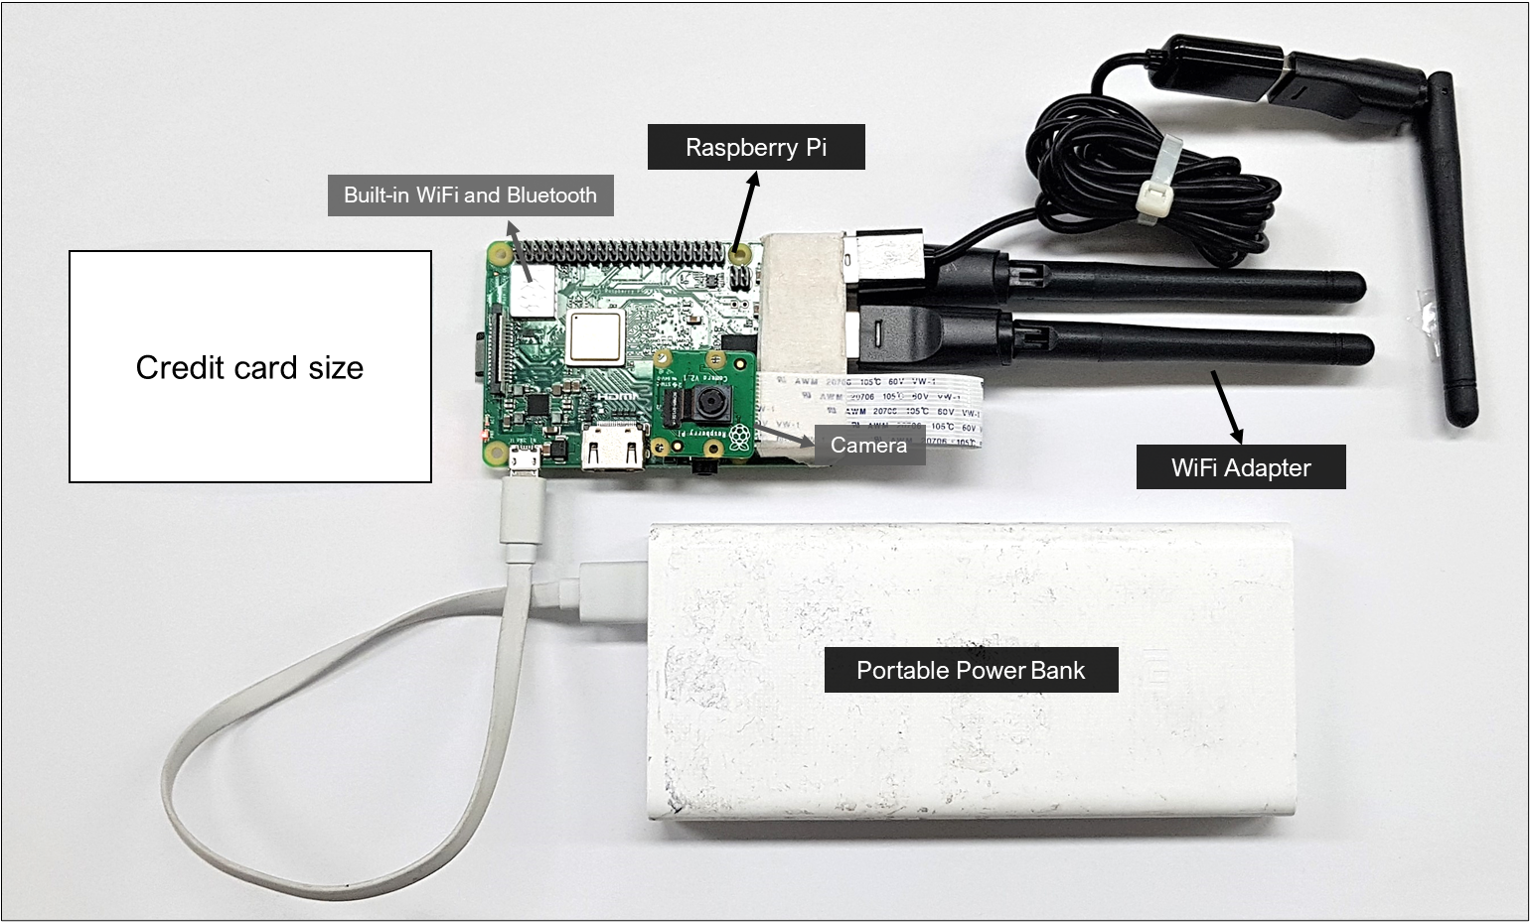
\includegraphics{content/material/ch2/sensor_comp.png}

The required hardware components for this WiFi sensor include:

\begin{longtable}[]{@{}
  >{\raggedright\arraybackslash}p{(\columnwidth - 4\tabcolsep) * \real{0.2119}}
  >{\raggedright\arraybackslash}p{(\columnwidth - 4\tabcolsep) * \real{0.3898}}
  >{\raggedright\arraybackslash}p{(\columnwidth - 4\tabcolsep) * \real{0.3983}}@{}}
\toprule\noalign{}
\begin{minipage}[b]{\linewidth}\raggedright
Hardware
\end{minipage} & \begin{minipage}[b]{\linewidth}\raggedright
Description
\end{minipage} & \begin{minipage}[b]{\linewidth}\raggedright
Specific Recommendation
\end{minipage} \\
\midrule\noalign{}
\endhead
\bottomrule\noalign{}
\endlastfoot
Raspberry Pi board & Core of our sensor & Pi 3B/3B+ or higher \\
WiFi adapter & Captures WiFi packets & Check chipset compatibility for
`monitoring mode' \\
Micro SD card and adapter & For system building and data storage & At
least 16 GB \\
Laptop and Ethernet cable & For accessing and controlling the sensor &
--- \\
Portable power bank & Powers the sensor in outdoor environments &
Battery capacity: +20,000 mAh \\
\end{longtable}

Besides these essentials, other hardware components may be attached to
the sensor depending on your project requirements, such as:

\begin{itemize}
\tightlist
\item
  \textbf{Pi camera:} This can be used to record the scene in front of
  the sensor.
\item
  \textbf{Air pollution sensor:} If you want to monitor air quality in
  addition to WiFi sensing. Temperature and humidity sensor: Useful for
  environmental monitoring and adjusting sensor performance based on
  climatic changes.
\item
  \textbf{Temperature and humidity sensor:} Useful for environmental
  monitoring and adjusting sensor performance based on climatic changes.
\end{itemize}

\section{Required Software}\label{required-software}

The key software programs necessary to build a WiFi sensor and manage
the sensor data are:

\begin{longtable}[]{@{}
  >{\raggedright\arraybackslash}p{(\columnwidth - 4\tabcolsep) * \real{0.2500}}
  >{\raggedright\arraybackslash}p{(\columnwidth - 4\tabcolsep) * \real{0.3194}}
  >{\raggedright\arraybackslash}p{(\columnwidth - 4\tabcolsep) * \real{0.4306}}@{}}
\toprule\noalign{}
\begin{minipage}[b]{\linewidth}\raggedright
Software
\end{minipage} & \begin{minipage}[b]{\linewidth}\raggedright
Purpose
\end{minipage} & \begin{minipage}[b]{\linewidth}\raggedright
Download Link
\end{minipage} \\
\midrule\noalign{}
\endhead
\bottomrule\noalign{}
\endlastfoot
Raspberry Pi Imager & Tool for writing Pi OS images onto SD cards &
\href{https://www.putty.org/}{Link} \\
DB Browser for SQLite & Tool for view database written as SQLlite (WiFi
packet file type) & \href{https://sqlitebrowser.org/}{Link} \\
\end{longtable}

Feel free to download these programs in advance. If needed, we will
provide the download links again when each step requires these tools.

\section{Necessary Skills}\label{necessary-skills}

Basic programming skills, specifically in R and Python, are required.
You should be able to write, edit, and debug code. To improve these
skills, consider the following courses:

\begin{itemize}
\tightlist
\item
  \href{https://www.coursera.org/specializations/data-science-foundations-r}{Data
  Science: Foundations using R Specialization} for a strong foundation
  in data science using R.
\item
  \href{https://www.coursera.org/specializations/python}{Python for
  Everybody Specialization} to learn programming basics in Python.
\end{itemize}

\chapter{Initial Setup}\label{initial-setup}

This segment guides you through the complete process of setting up a
Raspberry Pi, including the installation of the operating system
\emph{(2.1)}, various methods for connecting and accessing your Pi
remotely \emph{(2.2, 2.3, 2.4, 2.5)}. Additional troubleshooting and
advanced setup tips are also provided in section \emph{(2.6)}.

\section{Setting Up the Raspberry Pi Operating
System}\label{setting-up-the-raspberry-pi-operating-system}

\subsection{Download the Pi Imager}\label{download-the-pi-imager}

Begin by downloading the Raspberry Pi Imager, a tool for installing the
operating system on your Pi. This software is available on the
\href{https://www.raspberrypi.com/software/}{official Raspberry Pi
website}. Select the version compatible with your operating system
(Windows, macOS, or Ubuntu) and install it on your computer.

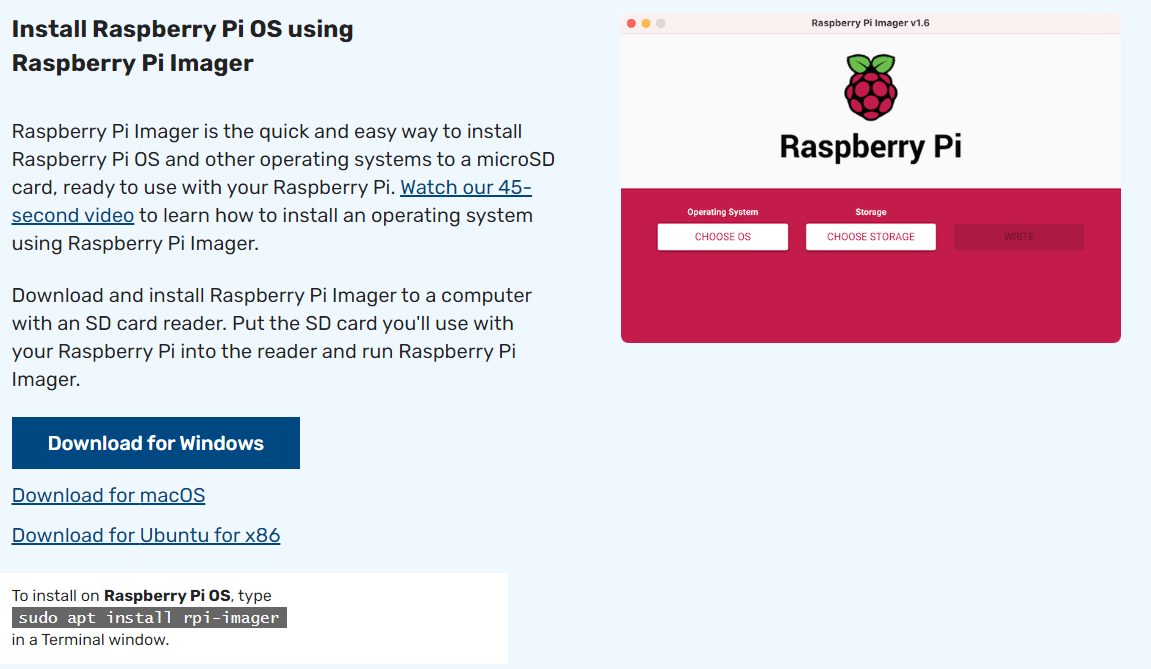
\includegraphics{content/material/ch2/raspi_imager.png}

\subsection{Format your SD Card}\label{format-your-sd-card}

Insert an SD card into your computer, then launch the Raspberry Pi
Imager you just installed. Click \texttt{CHOOSE\ OS}, then select the
\texttt{Erase} option followed by \texttt{Format\ SD\ Card}.

\includegraphics{content/material/ch2/format_SD.mp4}

\subsection{Flash the OS onto your SD
Card}\label{flash-the-os-onto-your-sd-card}

Once your SD card is formatted, you can proceed to install the Raspberry
Pi OS:

\begin{enumerate}
\def\labelenumi{\arabic{enumi}.}
\tightlist
\item
  \textbf{Open Raspberry Pi Imager} : Navigate back to the Raspberry Pi
  Imager main menu.
\item
  \textbf{Choose the OS} : Click \texttt{CHOOSE\ OS} and select the
  Raspberry Pi OS version you wish to install.
\item
  \textbf{Choose the SD Card} : Select \texttt{CHOOSE\ SD\ CARD} and
  pick your SD card from the list.
\item
  \textbf{Enable SSH} : This will allow remote access to the Raspberry
  Pi.
\item
  \textbf{Set Username and Password} : The Raspberry Pi OS's default
  username and password are `pi' and `raspberry'. For security reasons,
  it's advisable to change these once your system is up and running.
\item
  \textbf{Configure Wireless LAN} : This step allows you to connect with
  WiFi. For this project, you will use your mobile hotspot as a network
  provider. This will synchronize the Pi's time at boot by connecting to
  the network. Please set this up using your mobile hotspot information.
\item
  \textbf{Write the OS} : Finally, click \texttt{WRITE} to start the
  writing process. This will flash the selected OS onto your SD card.
\end{enumerate}

Please note that the exact steps for enabling SSH and configuring the
WLAN might vary depending on the version of the Raspberry Pi OS and the
Imager tool you are using. Refer to the specific documentation if you
encounter any issues.

\includegraphics{content/material/ch2/write_SD.mp4}

Once the process is complete, your SD card will be ready, and you can
insert it into the Raspberry Pi to boot up the new operating system.

\begin{tcolorbox}[enhanced jigsaw, opacityback=0, colbacktitle=quarto-callout-note-color!10!white, toptitle=1mm, colframe=quarto-callout-note-color-frame, rightrule=.15mm, title=\textcolor{quarto-callout-note-color}{\faInfo}\hspace{0.5em}{Why Do We Use Our Mobile Hotspot for This Project?}, toprule=.15mm, colback=white, bottomrule=.15mm, coltitle=black, breakable, leftrule=.75mm, left=2mm, opacitybacktitle=0.6, bottomtitle=1mm, arc=.35mm, titlerule=0mm]

The Raspberry Pi lacks a real-time clock, which means it can't keep
track of time when powered off. To fetch the current time when booting
up, it needs access to the internet. More details on this can be found
\href{https://dayne.broderson.org/2020/03/12/the_time_is_now.html}{here}.

To provide the necessary internet connection for time synchronization,
we'll use your mobile phone's hotspot. By establishing this connection,
the Raspberry Pi can easily access the current time, ensuring accurate
system operation. Here's how you can set up your hotspot:

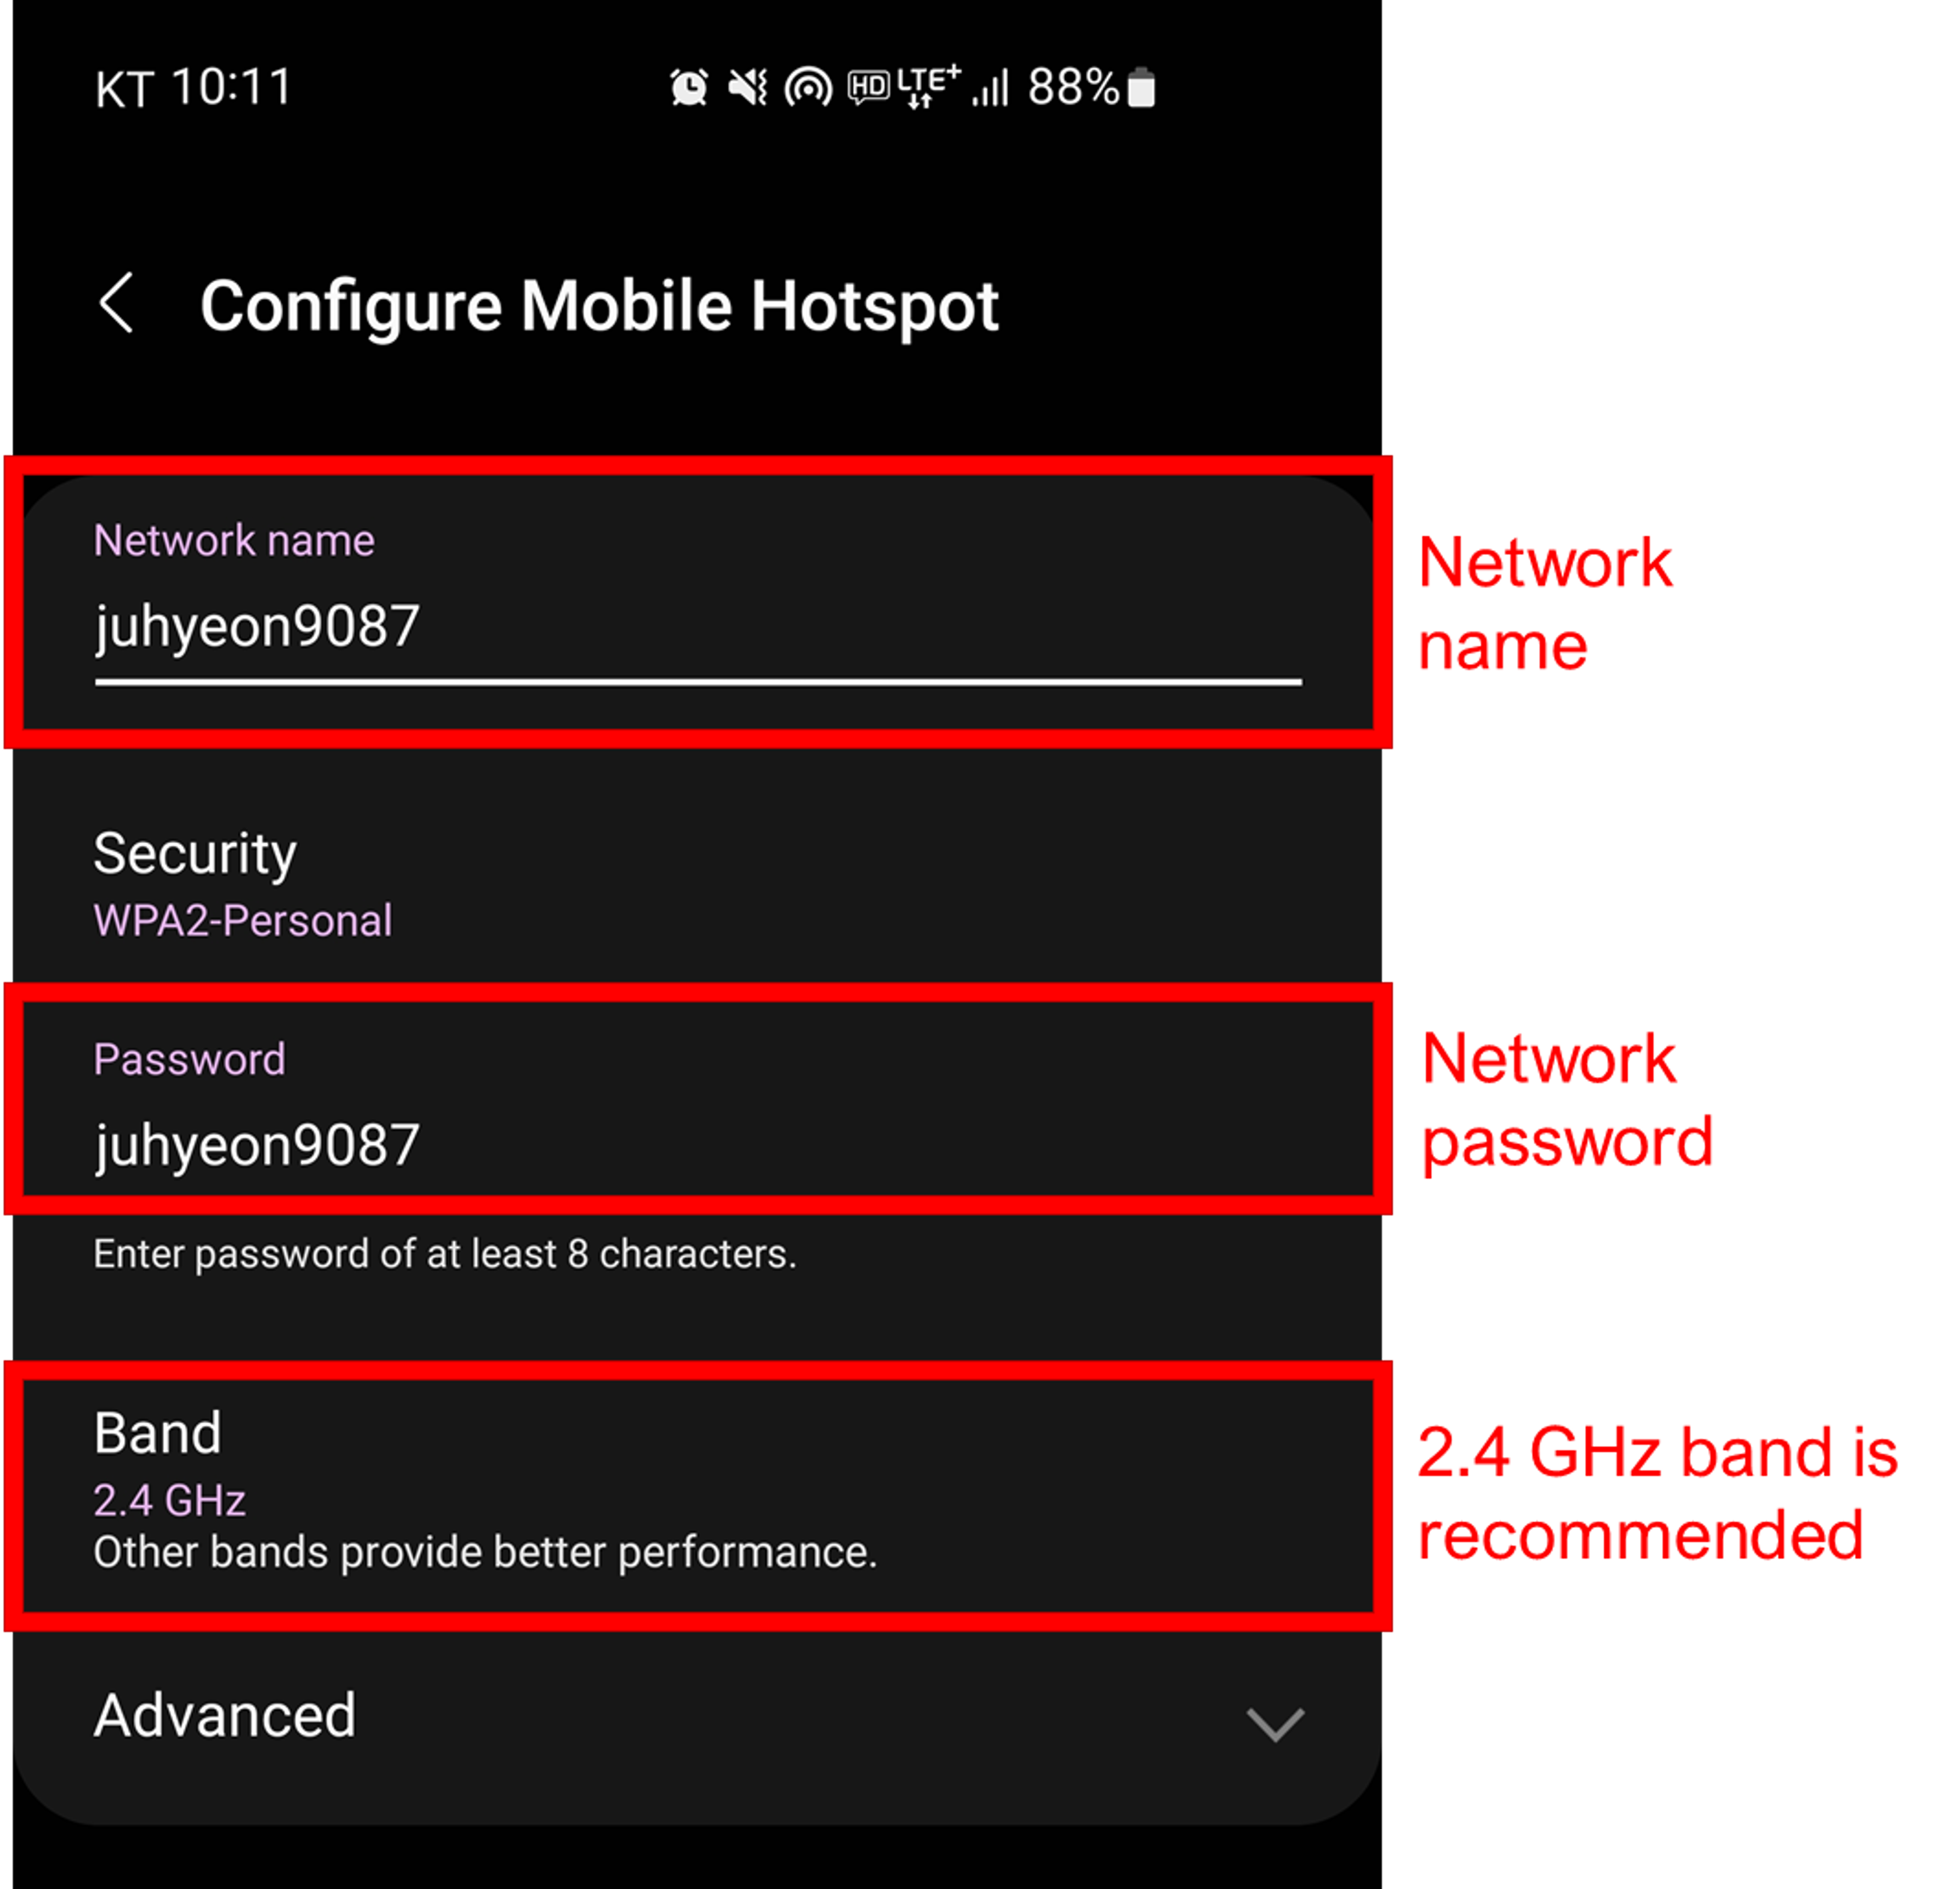
\includegraphics[width=0.5\textwidth,height=\textheight]{content/material/ch2/mobile_hotspot.png}

This approach leverages your mobile phone's data connection, creating a
seamless integration between the Raspberry Pi and the internet, which is
vital for the project's success.

\end{tcolorbox}

\section{Choose the Access Remotely
Way}\label{choose-the-access-remotely-way}

Choosing the correct method for remote access depends on your specific
setup and requirements. Below are the detailed instructions for both
methods, allowing smooth access and control of the Raspberry Pi:

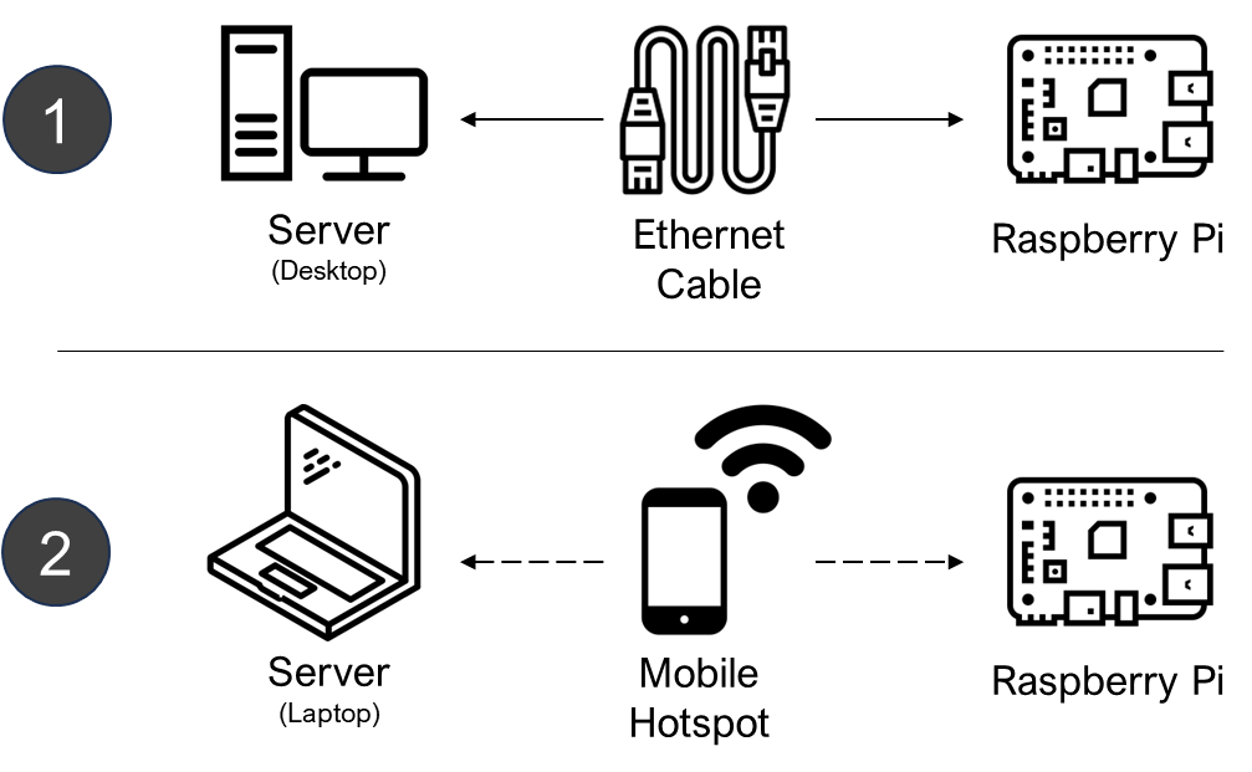
\includegraphics[width=0.85\textwidth,height=\textheight]{content/material/ch2/choose_remote.png}

\begin{itemize}
\item
  When you use a desktop (without WLAN card) to use access and control
  the Pi, choose the \texttt{(1)} and follow the instructions in Section
  2.2.4., Section~\ref{sec-way1}.
\item
  When you use a laptop (capable WLAN card) to use access and control
  the Pi, choose the \texttt{(2)} and follow the instructions in Section
  2.2.5., Section~\ref{sec-way2}.
\end{itemize}

\section{Access Your Pi Using an Ethernet Cable}\label{sec-way1}

\subsection{Connect your Pi to your
Laptop}\label{connect-your-pi-to-your-laptop}

With the Pi-equipped SD card, connect your Pi to your laptop using an
Ethernet cable.

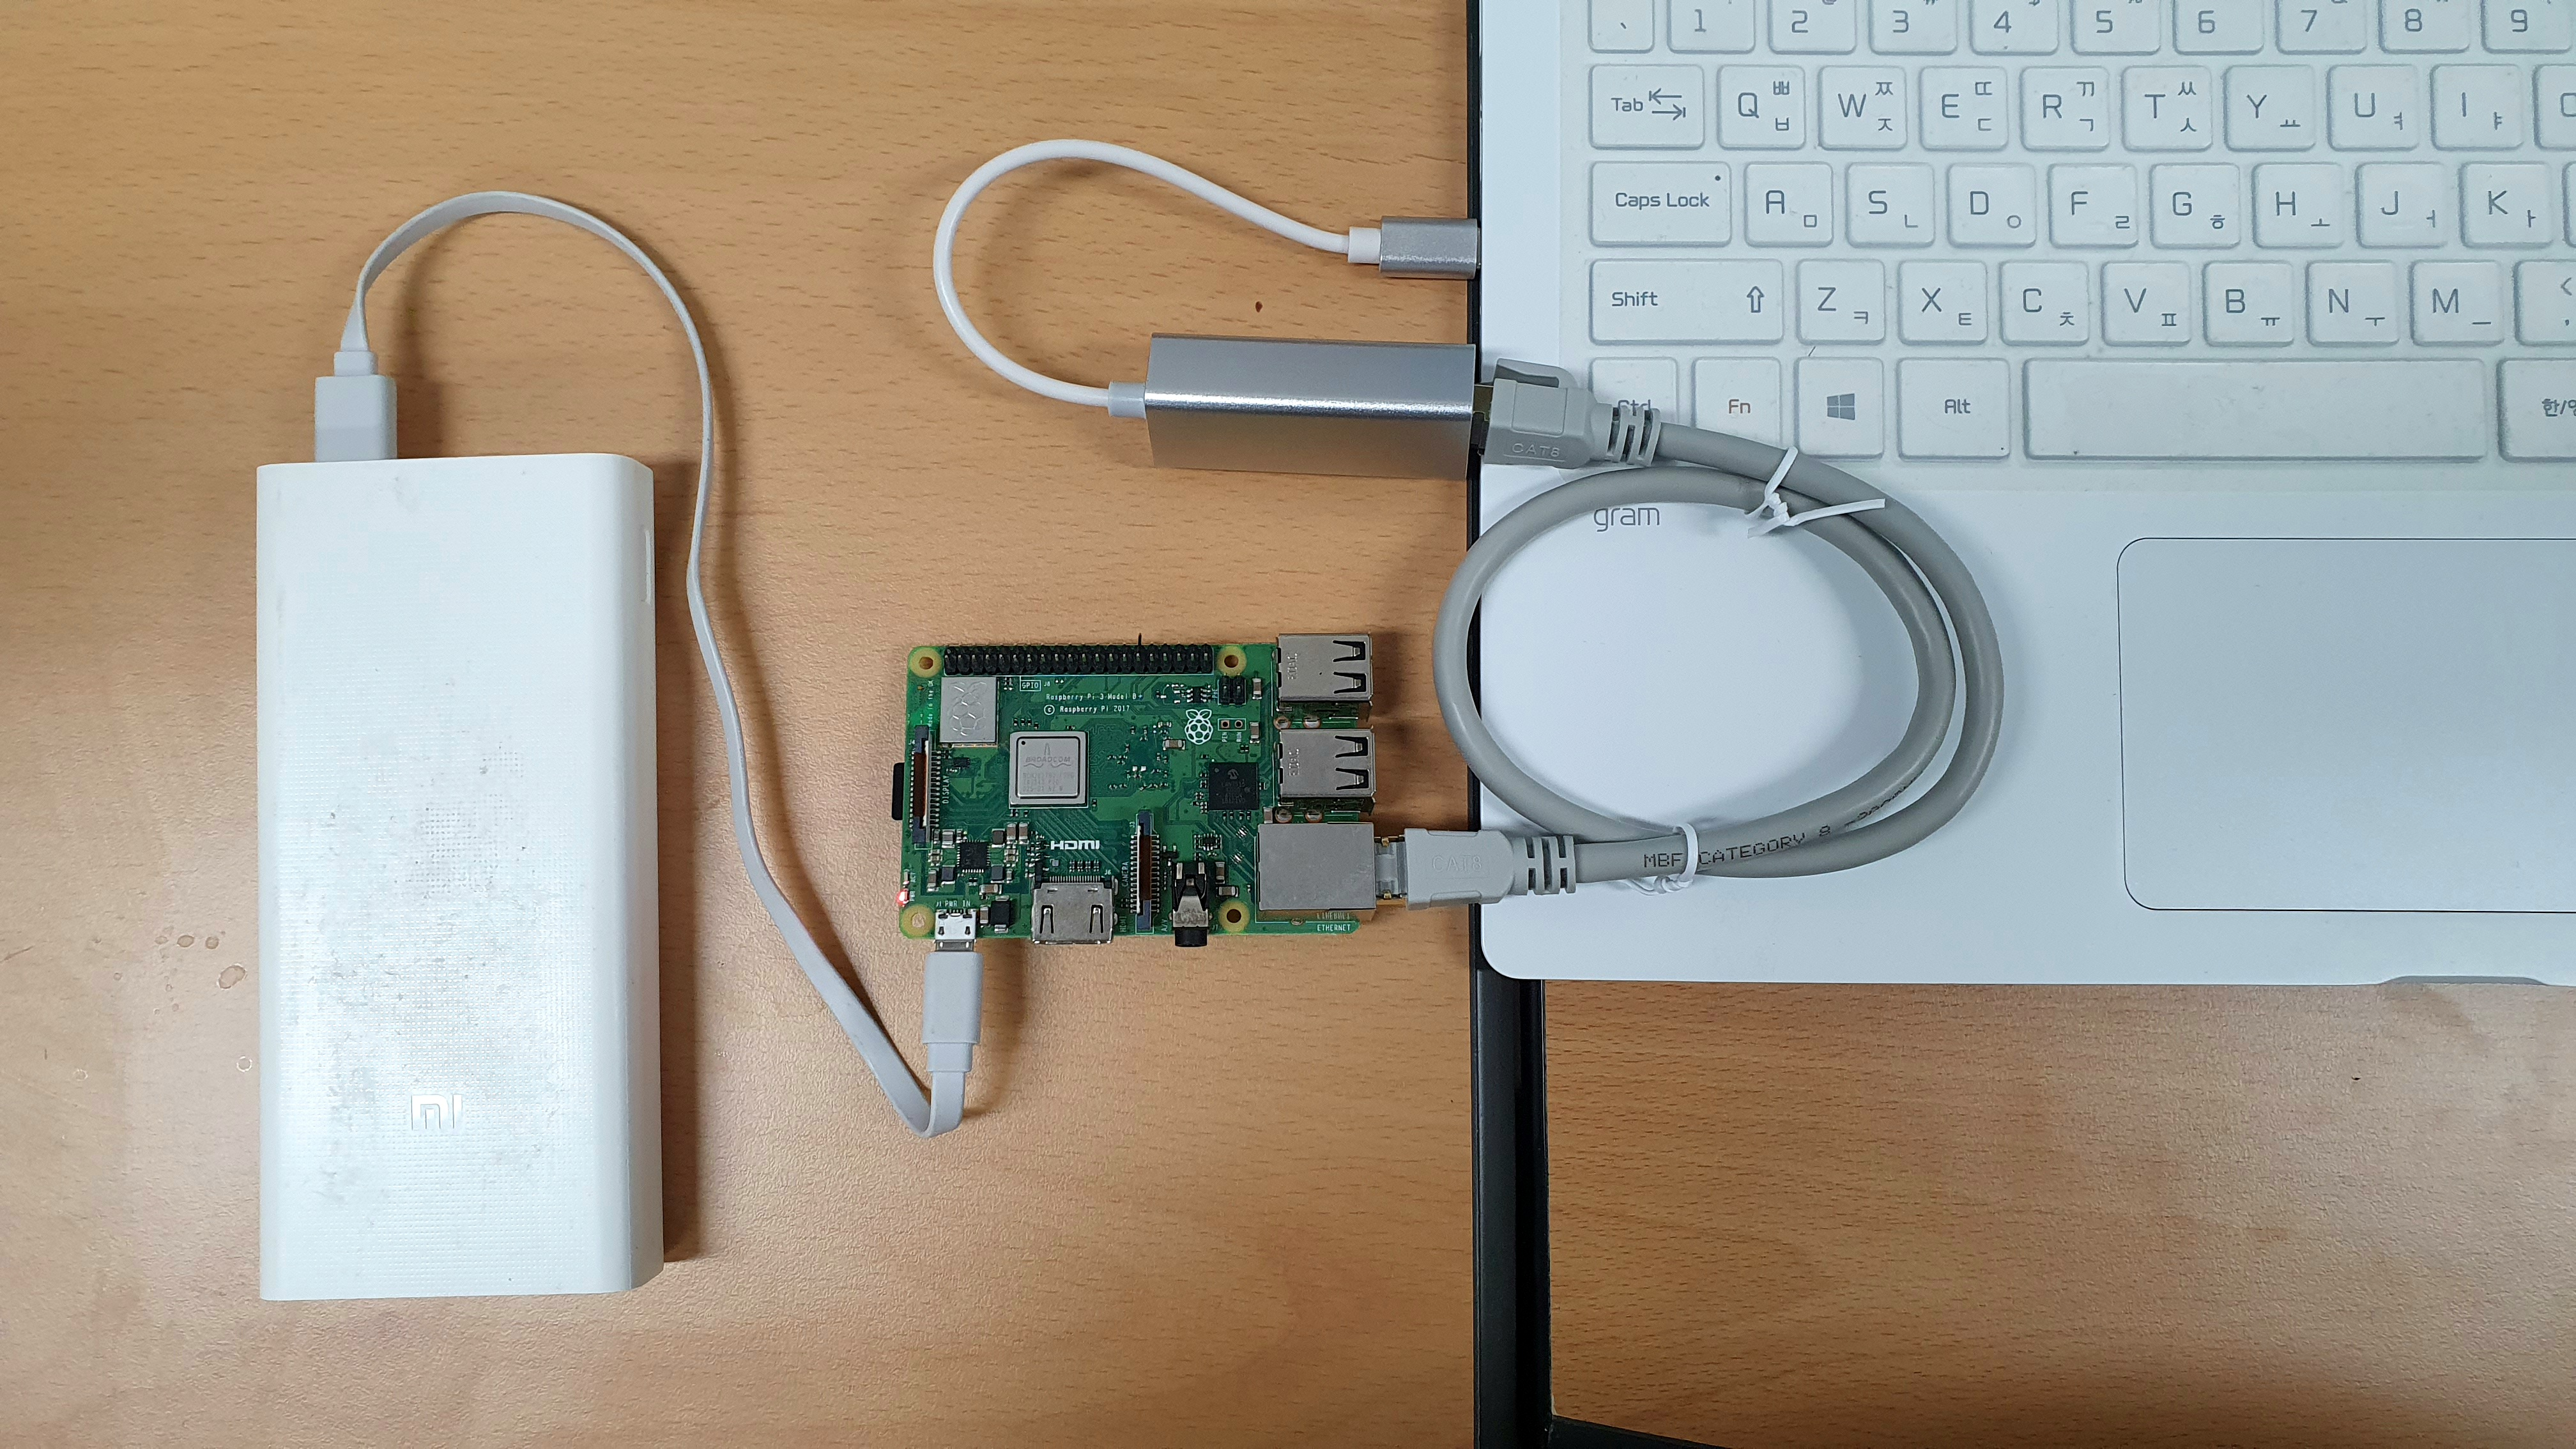
\includegraphics{content/material/ch2/connect_pi.jpg}

\subsection{Enable Internet Connection
Sharing}\label{enable-internet-connection-sharing}

Navigate to your laptop's network settings and enable the
\texttt{Internet\ Connection\ Sharing} option. This will allow your
laptop to share its internet connection with the Raspberry Pi via the
Ethernet cable, provided it's connected to the internet.

\includegraphics{content/material/ch2/share_network.mp4}

\subsection{Access Your Raspberry Pi via
SSH}\label{access-your-raspberry-pi-via-ssh}

Having installed the Windows Terminal from the Microsoft Store, you can
access the Command Prompt by pressing \texttt{Ctrl\ +\ R}, typing
\texttt{cmd}, and hitting \texttt{Enter}. Alternatively, you can open it
by pressing \texttt{Ctrl\ +\ Shift\ +\ P}. This is what you should see:

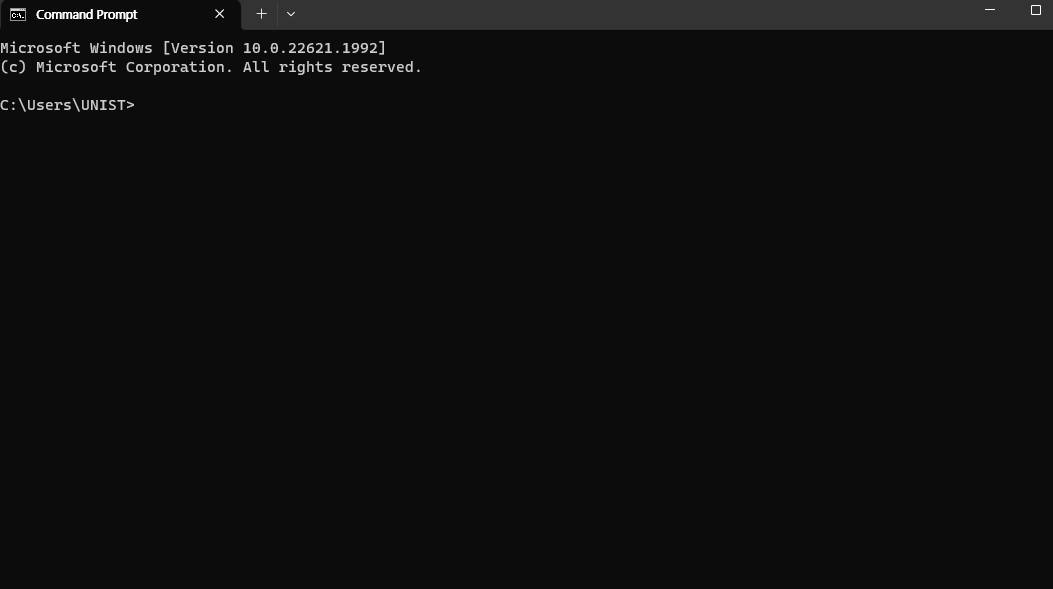
\includegraphics{content/material/ch2/cmd_screen.png}

To establish an SSH connection with your Raspberry Pi, enter the
following command:

\begin{Shaded}
\begin{Highlighting}[]
\FunctionTok{ssh}\NormalTok{ pi@raspberrypi}
\end{Highlighting}
\end{Shaded}

\includegraphics{content/material/ch2/access_cmd.mp4}

\begin{tcolorbox}[enhanced jigsaw, opacityback=0, colbacktitle=quarto-callout-note-color!10!white, toptitle=1mm, colframe=quarto-callout-note-color-frame, rightrule=.15mm, title=\textcolor{quarto-callout-note-color}{\faInfo}\hspace{0.5em}{Note}, toprule=.15mm, colback=white, bottomrule=.15mm, coltitle=black, breakable, leftrule=.75mm, left=2mm, opacitybacktitle=0.6, bottomtitle=1mm, arc=.35mm, titlerule=0mm]

If you encounter any troubles with this section, please refer to the
last section of this content, titled \textbf{Issues of Initial Setup},
for guidance and solutions.

\end{tcolorbox}

\section{Access Your Pi Using Your Phone as a Network
Provider}\label{sec-way2}

\subsection{Set Up Your Mobile
Hotspot}\label{set-up-your-mobile-hotspot}

Enable your mobile hotspot with the same settings you used when flashing
the SD card:

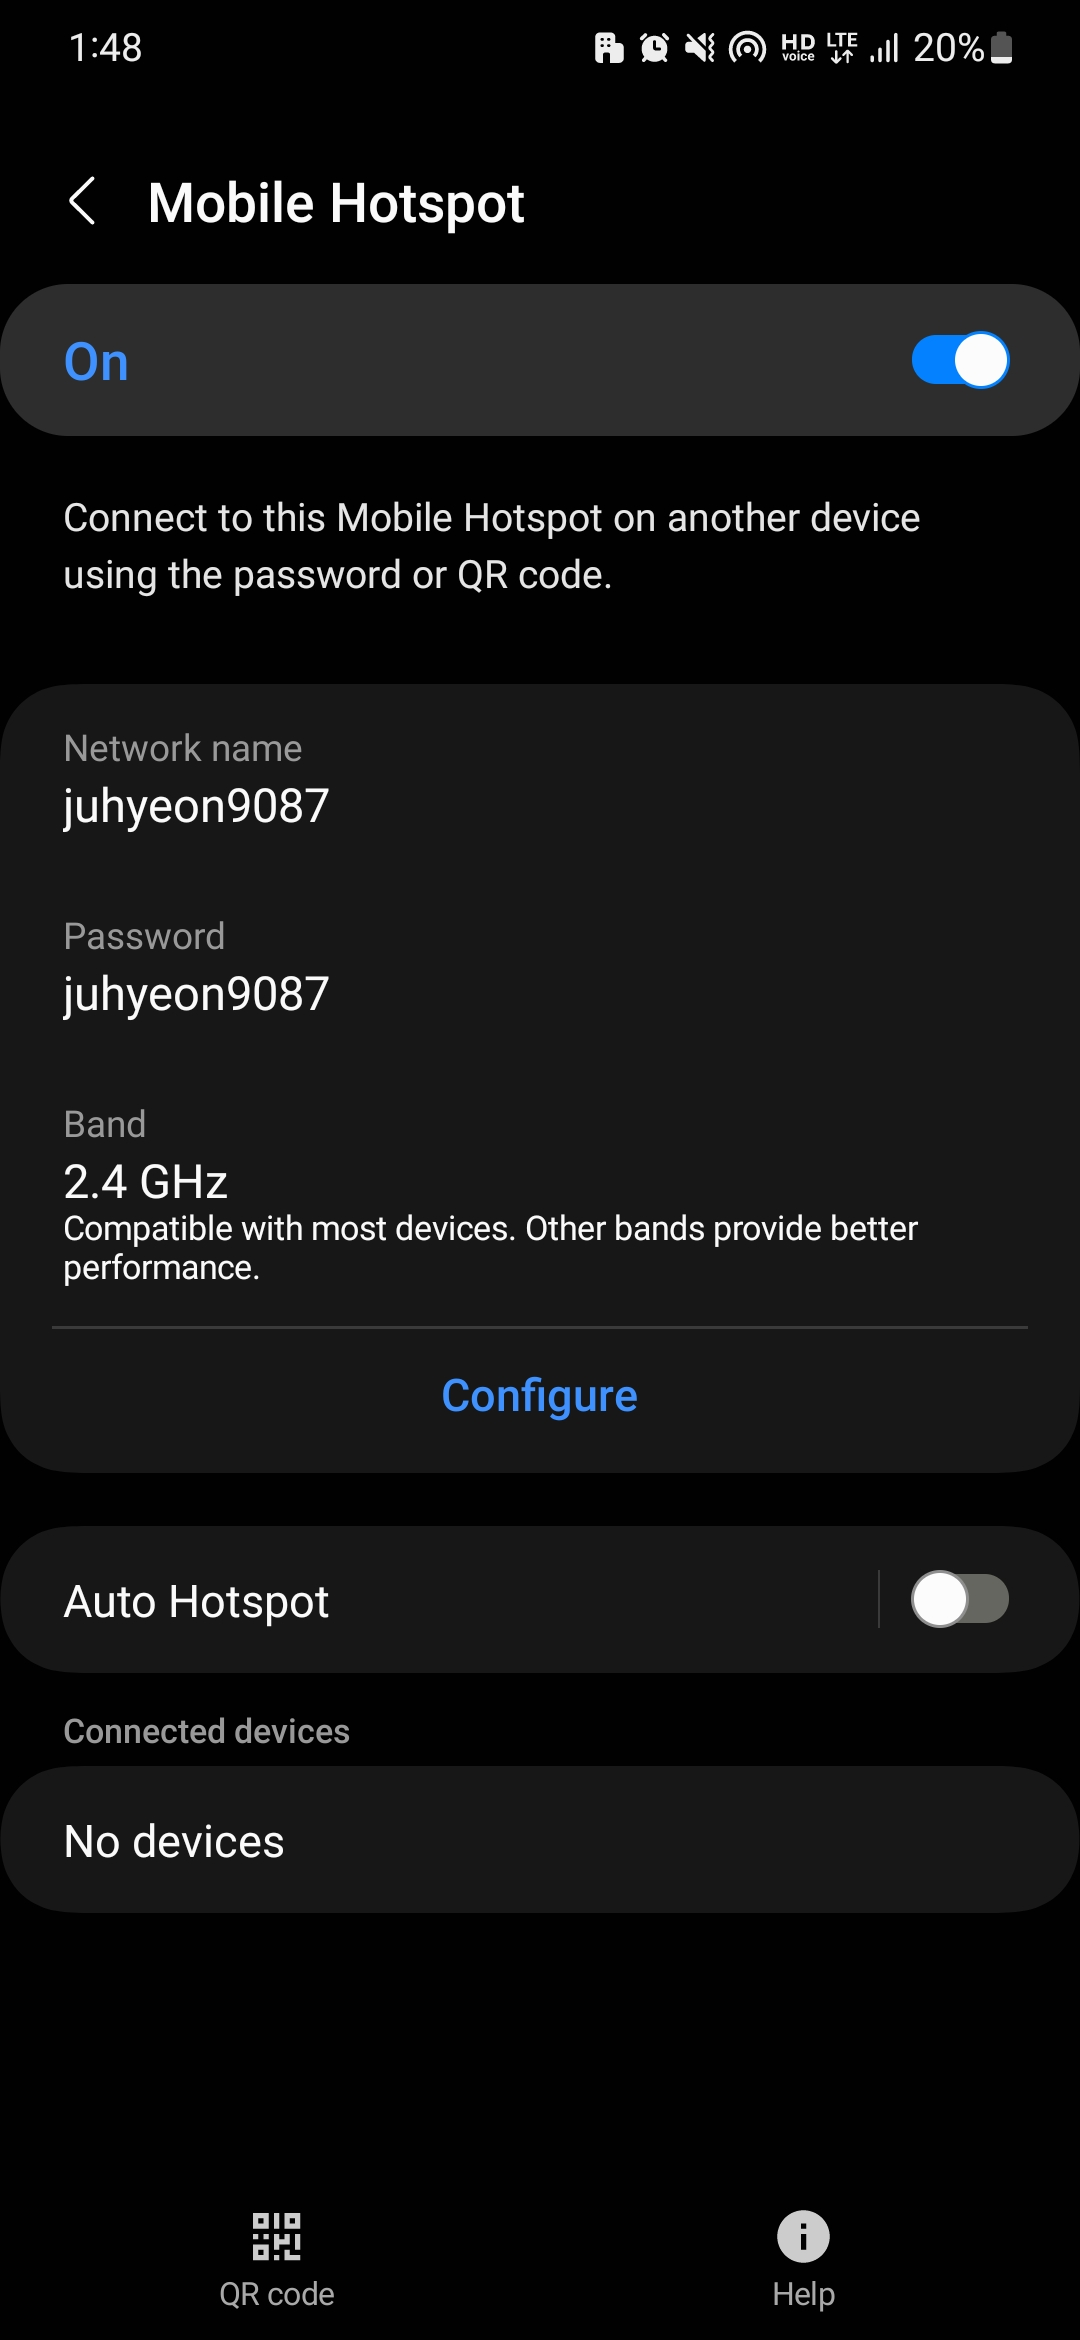
\includegraphics[width=0.5\textwidth,height=\textheight]{content/material/ch2/hotspot_default.jpg}

\subsection{Power Up Your Pi}\label{power-up-your-pi}

Insert the prepared SD card into your Pi and plug in the power:

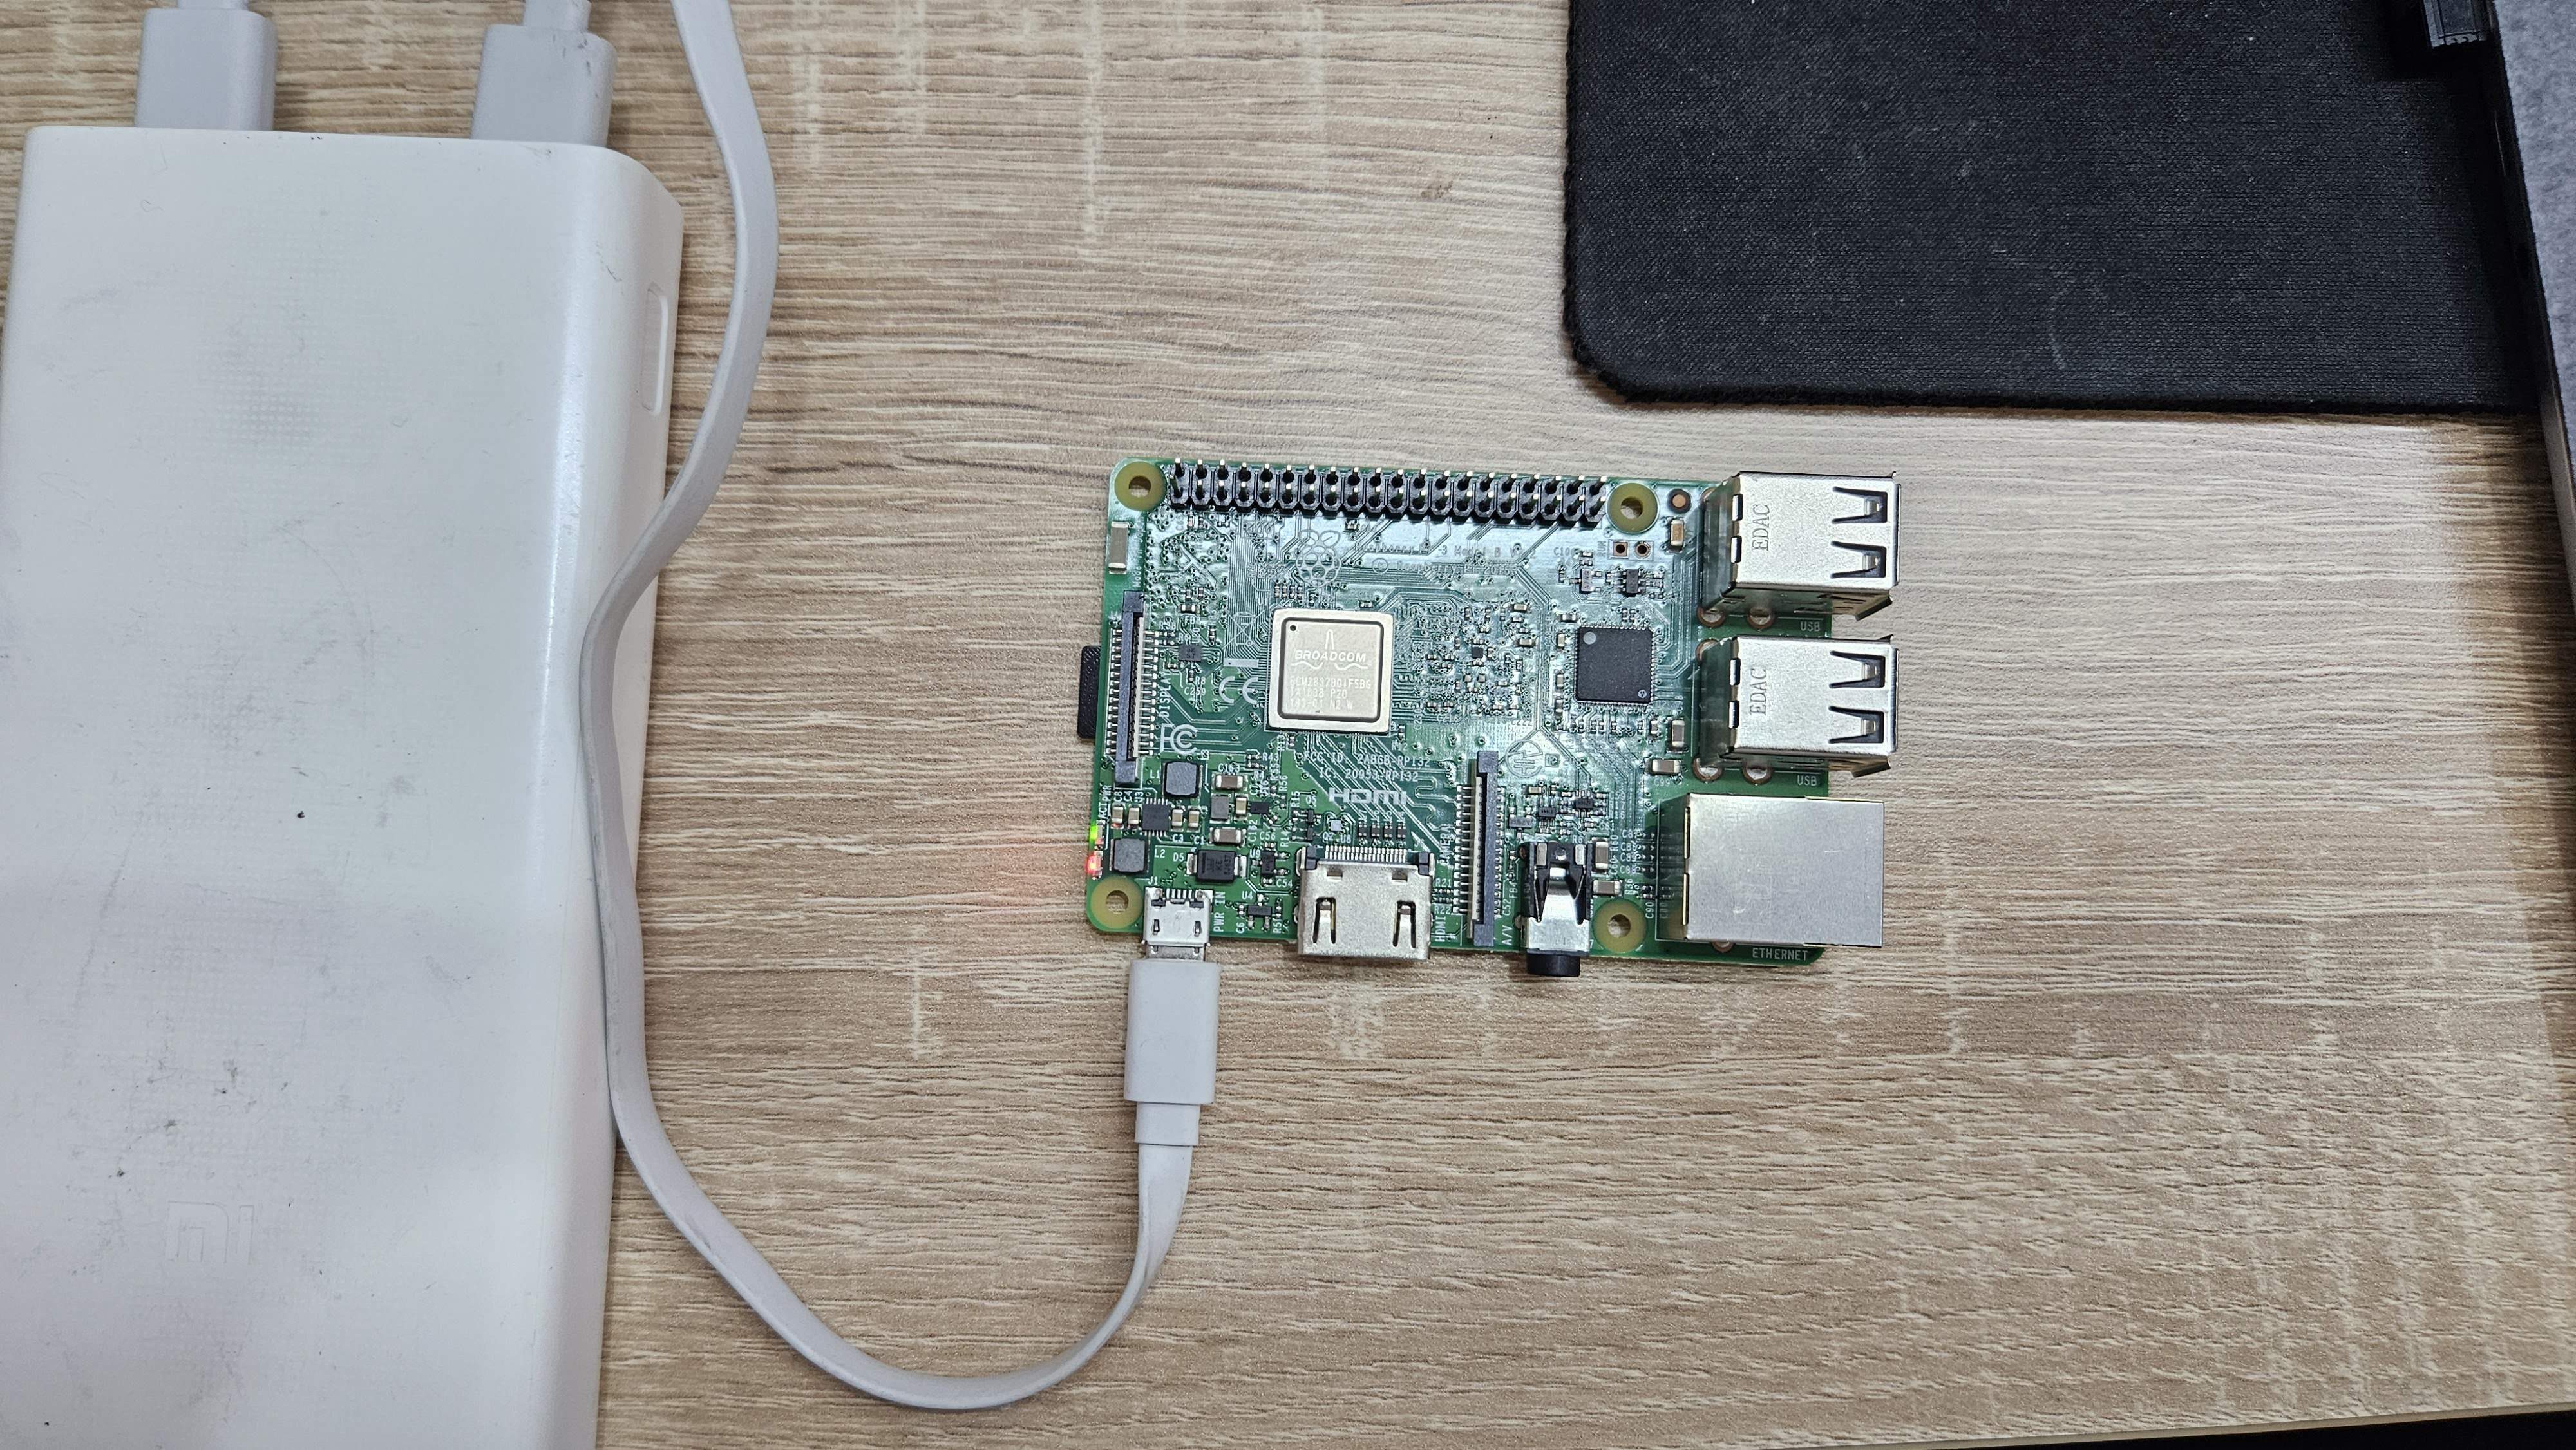
\includegraphics{content/material/ch2/plug_pi_wifi.jpg}

\subsection{Connect Your Laptop to Your Mobile
Hotspot}\label{connect-your-laptop-to-your-mobile-hotspot}

Configure your laptop's WiFi to connect to the mobile hotspot:

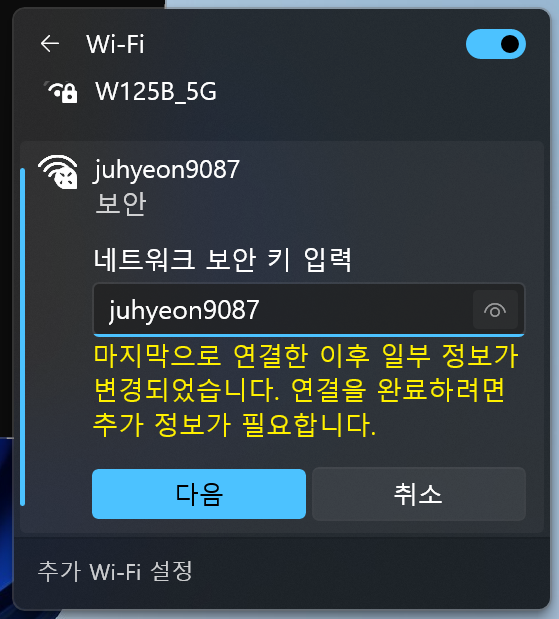
\includegraphics[width=0.5\textwidth,height=\textheight]{content/material/ch2/laptop_wifi.png}

\subsection{Verify Connections in Your Mobile Hotspot
Interface}\label{verify-connections-in-your-mobile-hotspot-interface}

After waiting a few seconds, you should see two connected devices in
your interface:

\textbf{1. raspberrypi:} The Raspberry Pi - after waiting a few seconds,
you should see the Raspberry Pi appear in your mobile hotspot interface.

\textbf{2. your laptop:} Your laptop's name, as it appears on the
network.

\subsection{Access Your Pi via SSH}\label{access-your-pi-via-ssh}

First, open the Command Prompt. If you have installed the Windows
Terminal from the Microsoft Store, you can access the Command Prompt by
pressing Ctrl + R, typing cmd, and hitting Enter. Alternatively, you can
open it by pressing Ctrl + Shift + P. You should see the following:

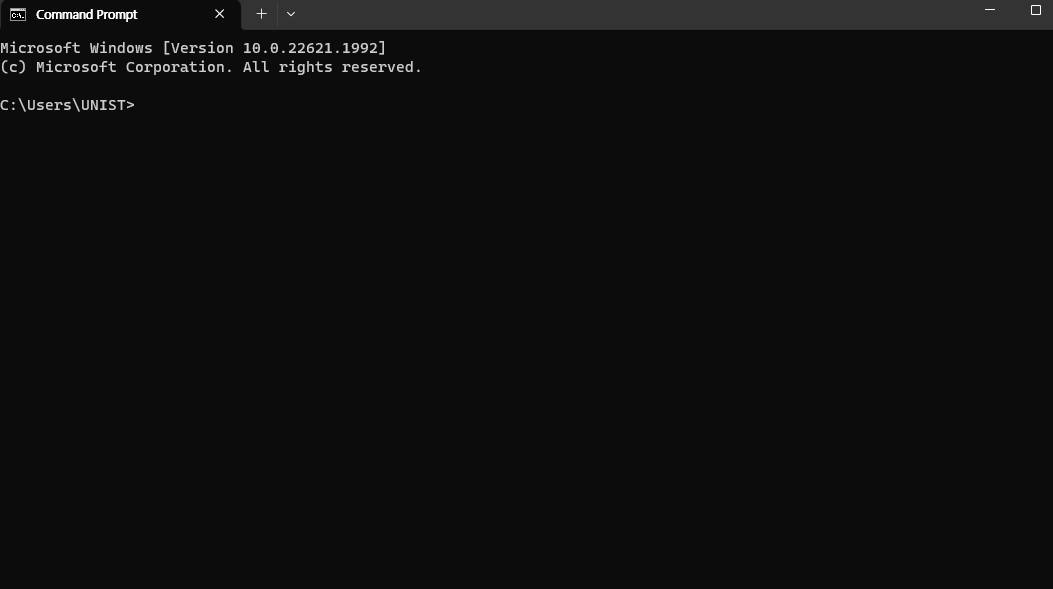
\includegraphics{content/material/ch2/cmd_screen.png}

Now, establish an SSH connection with your Raspberry Pi by entering this
command:

\begin{Shaded}
\begin{Highlighting}[]
\FunctionTok{ssh}\NormalTok{ pi@raspberrypi}
\end{Highlighting}
\end{Shaded}

\includegraphics{content/material/ch2/ssh_laptop.mp4}

\begin{tcolorbox}[enhanced jigsaw, opacityback=0, colbacktitle=quarto-callout-note-color!10!white, toptitle=1mm, colframe=quarto-callout-note-color-frame, rightrule=.15mm, title=\textcolor{quarto-callout-note-color}{\faInfo}\hspace{0.5em}{Note}, toprule=.15mm, colback=white, bottomrule=.15mm, coltitle=black, breakable, leftrule=.75mm, left=2mm, opacitybacktitle=0.6, bottomtitle=1mm, arc=.35mm, titlerule=0mm]

If you encounter any troubles with this section, please refer to the
last section of this content, titled \textbf{Issues of Initial Setup},
for guidance and solutions.

\end{tcolorbox}

\section{Verify Your Pi's Internet
Connectivity}\label{verify-your-pis-internet-connectivity}

To confirm your Raspberry Pi's internet connection, use the ping command
followed by the IP address of a well-known site. For example, ping
Google's Public DNS Server by typing this command:

\begin{Shaded}
\begin{Highlighting}[]
\FunctionTok{ping}\NormalTok{ 8.8.8.8}
\end{Highlighting}
\end{Shaded}

If the Pi is connected to the internet, you will see lines starting with
`64 bytes from 8.8.8.8' and a summary of the ping at the end.

\includegraphics{content/material/ch2/cmd_ping.mp4}

You can stop the ping process by pressing \texttt{Ctrl\ +\ C}.

\begin{tcolorbox}[enhanced jigsaw, opacityback=0, colbacktitle=quarto-callout-note-color!10!white, toptitle=1mm, colframe=quarto-callout-note-color-frame, rightrule=.15mm, title=\textcolor{quarto-callout-note-color}{\faInfo}\hspace{0.5em}{Note}, toprule=.15mm, colback=white, bottomrule=.15mm, coltitle=black, breakable, leftrule=.75mm, left=2mm, opacitybacktitle=0.6, bottomtitle=1mm, arc=.35mm, titlerule=0mm]

If you encounter any troubles with this section, please refer to the
last section of this content, titled \textbf{Issues of Initial Setup},
for guidance and solutions.

\end{tcolorbox}

\section{Issues of initial setup}\label{issues-of-initial-setup}

\subsection{Connection and network
error}\label{connection-and-network-error}

If you encounter any errors accessing your Pi or the internet
connectivity, please follow these steps:

\begin{enumerate}
\def\labelenumi{\arabic{enumi}.}
\tightlist
\item
  Enable and then disable the network on your laptop or desktop
  computer.
\item
  Check and uncheck the ``Enable Internet Connection Sharing'' function
  in your network settings.
\item
  Verify the network connection made by your Pi through the Ethernet.
\end{enumerate}

\includegraphics{content/material/ch2/error_network.mp4}

\subsection{Locating Your Raspberry Pi's IP Address using MAC
Address}\label{locating-your-raspberry-pis-ip-address-using-mac-address}

If you need to access your Pi with a specific IP address, especially
when connected to multiple Pis, follow these guidelines:

\textbf{1. Open Command Prompt:} Press the \texttt{Windows} key on your
keyboard, type \texttt{cmd} and hit \texttt{Enter}.

\textbf{2. Execute the \texttt{arp\ -a} command:} This command displays
the IP and MAC addresses of devices on your network.

\textbf{3. Identify your Raspberry Pi:} Raspberry Pi devices have MAC
addresses that start with \texttt{B8:27:EB:xx:xx:xx} or
\texttt{DC:A6:32:xx:xx:xx}. Find the device in the list with a physical
address that starts with these characters - that's your Raspberry Pi's
IP address.

\textbf{Note:} These are the MAC address prefixes specific to Raspberry
Pi Foundation devices. Your device's MAC address may start with a
different prefix.

\includegraphics{content/material/ch2/access_with_mac.mp4}

\subsection{`WARNING: REMOTE HOST IDENTIFICATION HAS
CHANGED!'}\label{warning-remote-host-identification-has-changed}

This warning appears when the remote system has different identification
than expected, such as after a system re-installation or SSH key change.

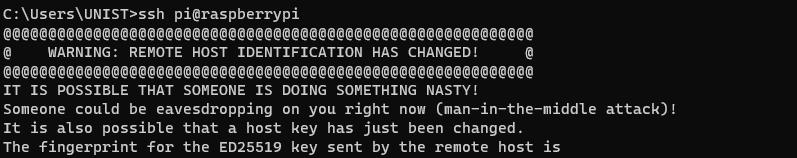
\includegraphics{content/material/ch2/ssh_error.png}

You can fix this error by removing the old key for the Raspberry Pi:

\begin{Shaded}
\begin{Highlighting}[]
\FunctionTok{ssh{-}keygen} \AttributeTok{{-}R}\NormalTok{ raspberrypi}
\end{Highlighting}
\end{Shaded}

Afterwards, try to re-establish the SSH connection.

\subsection{Using an Enhanced Security
Network}\label{using-an-enhanced-security-network}

If you're on a network with higher security, you may need to register
your Raspberry Pi's MAC address. See the example below from a university
network and consult with your network administrator or IT support for
your specific procedures.

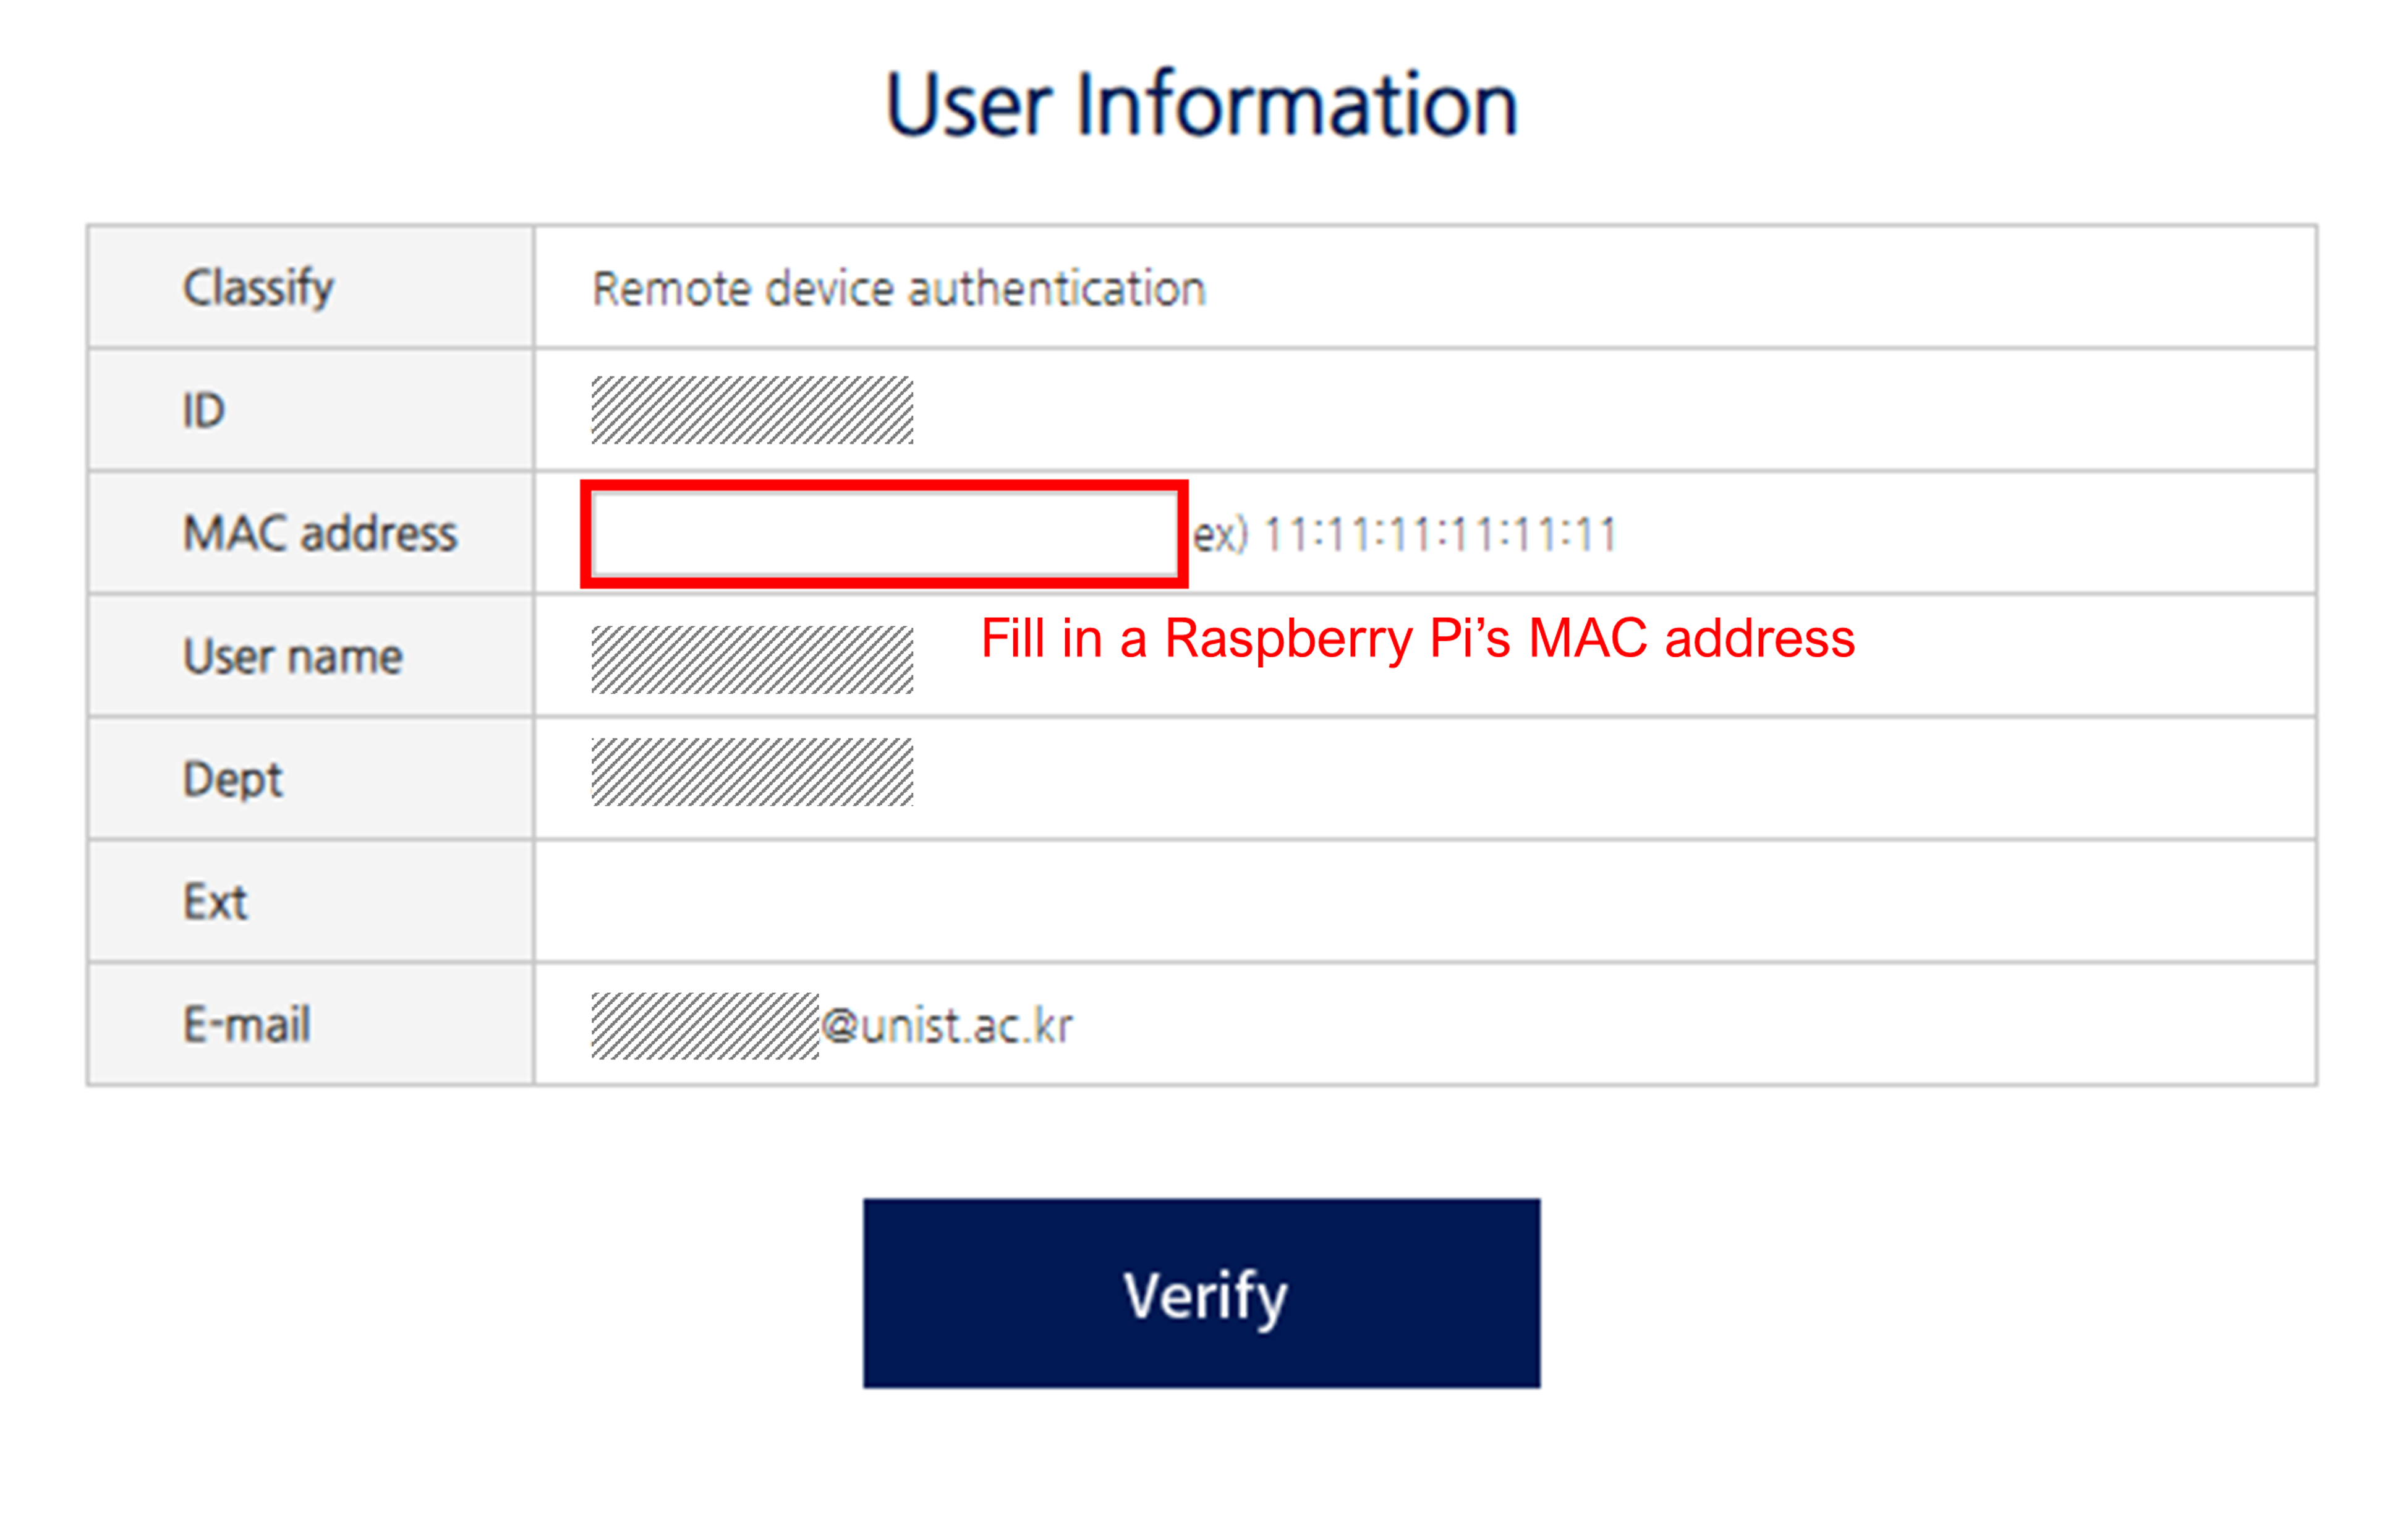
\includegraphics[width=5.20833in,height=\textheight]{content/material/ch2/network_unist.png}

\chapter{Raspberry Pi Setup}\label{raspberry-pi-setup}

This section covers preparing your Raspberry Pi OS \emph{(3.1)},
transforming it into a file server for easy file sharing \emph{(3.2)},
and configuring it to send status updates to cloud storage for remote
monitoring \emph{(3.3)}.

\section{Prepare Your Raspberry Pi
OS}\label{prepare-your-raspberry-pi-os}

\subsection{Update Your Pi}\label{update-your-pi}

Start by updating your Raspberry Pi's operating system (OS) to its
latest version. Open a terminal window and enter the following commands:

\begin{Shaded}
\begin{Highlighting}[]
\FunctionTok{sudo}\NormalTok{ apt{-}get update }\AttributeTok{{-}y} \KeywordTok{\&\&} \FunctionTok{sudo}\NormalTok{ apt{-}get upgrade }\AttributeTok{{-}y}
\end{Highlighting}
\end{Shaded}

\begin{tcolorbox}[enhanced jigsaw, opacityback=0, colbacktitle=quarto-callout-note-color!10!white, toptitle=1mm, colframe=quarto-callout-note-color-frame, rightrule=.15mm, title=\textcolor{quarto-callout-note-color}{\faInfo}\hspace{0.5em}{How to copy/paste in Linux terminal}, toprule=.15mm, colback=white, bottomrule=.15mm, coltitle=black, breakable, leftrule=.75mm, left=2mm, opacitybacktitle=0.6, bottomtitle=1mm, arc=.35mm, titlerule=0mm]

For copy, you could click this icon to copy the command:

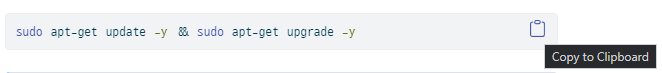
\includegraphics{content/material/ch2/ex_copy.png}

For paste, there are various ways; please visit
\href{https://www.maketecheasier.com/enable-copy-paste-command-prompt-windows10/}{this}
when Ctrl+V doesn't work in the terminal.

\end{tcolorbox}

\begin{tcolorbox}[enhanced jigsaw, opacityback=0, colbacktitle=quarto-callout-note-color!10!white, toptitle=1mm, colframe=quarto-callout-note-color-frame, rightrule=.15mm, title=\textcolor{quarto-callout-note-color}{\faInfo}\hspace{0.5em}{Note}, toprule=.15mm, colback=white, bottomrule=.15mm, coltitle=black, breakable, leftrule=.75mm, left=2mm, opacitybacktitle=0.6, bottomtitle=1mm, arc=.35mm, titlerule=0mm]

In Linux systems, \texttt{sudo} stands for ``superuser do'', similar to
``Run As Administrator'' in Windows. The \texttt{-y} flag automatically
confirms any prompts during the update process. The
\texttt{apt-get\ update} command refreshes the list of available
packages and their versions, while \texttt{apt-get\ upgrade} installs
the latest versions. You can learn basic Linux commands on websites like
\href{https://www.hostinger.com/tutorials/linux-commands}{this}.

\end{tcolorbox}

The given command should be placed like this:

\includegraphics{content/material/ch2/initial_update.mp4}

After the updates are complete, restart your Raspberry Pi using this
command:

\begin{Shaded}
\begin{Highlighting}[]
\FunctionTok{sudo}\NormalTok{ reboot}
\end{Highlighting}
\end{Shaded}

\subsection{Update Your Pi}\label{update-your-pi-1}

Before starting any kind of system-wide transformation, it's important
to have the necessary administrative privileges. On Raspberry Pi, you
can enter the superuser mode (or root mode) by using the command:

\begin{Shaded}
\begin{Highlighting}[]
\FunctionTok{sudo}\NormalTok{ su}
\end{Highlighting}
\end{Shaded}

\section{Transforming Your Pi into a File
Server}\label{transforming-your-pi-into-a-file-server}

This process allows \textbf{easy sharing of files between a Raspberry Pi
and other devices,} such as laptops and PCs. \texttt{Samba}, an
open-source secure network file-sharing system, enables this transfer.
By setting up Samba, files can be conveniently transferred to and from a
laptop within your network to a Raspberry Pi, via a direct Ethernet
connection.

\subsection{Install Samba}\label{install-samba}

Enter the following command in your terminal to install Samba:

\begin{Shaded}
\begin{Highlighting}[]
\FunctionTok{sudo}\NormalTok{ apt{-}get install }\AttributeTok{{-}y} \AttributeTok{{-}q}\NormalTok{ samba samba{-}common{-}bin}
\end{Highlighting}
\end{Shaded}

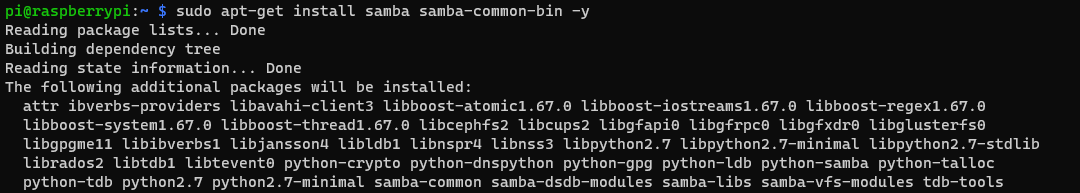
\includegraphics{content/material/ch2/install_samba.png}

\subsection{Modify the Samba Config
File}\label{modify-the-samba-config-file}

To share the Pi's folder, modify the Samba config file using the
following command:

\begin{Shaded}
\begin{Highlighting}[]
\FunctionTok{sudo}\NormalTok{ nano /etc/samba/smb.conf}
\end{Highlighting}
\end{Shaded}

Move to the end line by pressing \texttt{Alt\ +\ /} and add this:

\begin{Shaded}
\begin{Highlighting}[]
\OperatorTok{[}\NormalTok{share}\OperatorTok{]}
\NormalTok{path }\OperatorTok{=} \OperatorTok{/}\NormalTok{home}\OperatorTok{/}\NormalTok{pi}
\NormalTok{writeable}\OperatorTok{=}\NormalTok{Yes}
\NormalTok{create mast}\OperatorTok{=}\DecValTok{0777}
\DataTypeTok{directory}\NormalTok{ mast}\OperatorTok{=}\DecValTok{0777}
\DataTypeTok{public}\OperatorTok{=}\NormalTok{no}
\end{Highlighting}
\end{Shaded}

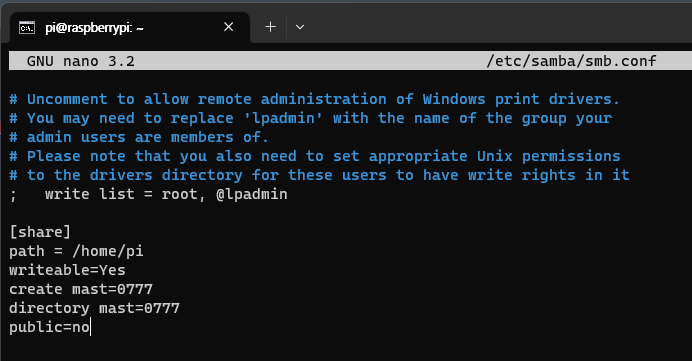
\includegraphics{content/material/ch2/samba_setting.png}

Press \texttt{Ctrl\ +\ X}, then \texttt{Y}, followed by \texttt{Enter}
to save the changes.

\subsection{Set Up a Samba User}\label{set-up-a-samba-user}

Set up a user for your Samba share on your Pi using this command:

\begin{Shaded}
\begin{Highlighting}[]
\FunctionTok{sudo}\NormalTok{ smbpasswd }\AttributeTok{{-}a}\NormalTok{ pi}
\end{Highlighting}
\end{Shaded}

Then, enter the password twice as prompted by the command. In this case,
the password is \texttt{raspberry}.

\subsection{Restart Samba Services}\label{restart-samba-services}

Restart the Samba services to apply the changes by typing this:

\begin{Shaded}
\begin{Highlighting}[]
\FunctionTok{sudo}\NormalTok{ service smbd restart}
\end{Highlighting}
\end{Shaded}

\begin{Shaded}
\begin{Highlighting}[]
\FunctionTok{sudo}\NormalTok{ service nmbd restart}
\end{Highlighting}
\end{Shaded}

\subsection{Access the Pi Directory}\label{access-the-pi-directory}

Open the File Explorer (press \texttt{Win\ +\ E}), type in the address
\texttt{raspberrypi/pi}, then enter the Pi's name and password as
network credentials.

\includegraphics{content/material/ch2/samba_access.mp4}

\subsection{Create and Verify the Test
File}\label{create-and-verify-the-test-file}

Create a text file in your Pi's directory using the following command.

\begin{Shaded}
\begin{Highlighting}[]
\FunctionTok{sudo}\NormalTok{ nano test.txt}
\end{Highlighting}
\end{Shaded}

After typing anything (e.g., `gg') in the file, press
\texttt{Ctrl\ +\ x}, then \texttt{y}, followed by \texttt{Enter}. You
should then be able to see the file on your laptop.

\includegraphics{content/material/ch2/samba_check.mp4}

\section{Setting Up Cloud Storage Access on Your
Pi}\label{setting-up-cloud-storage-access-on-your-pi}

This step involves \textbf{configuring your Raspberry Pi to send status
data to your cloud storage}. It's essential to ensure that your Pi is
properly set up before or during its installation. Typically, you might
consider connecting a monitor, mouse, and keyboard to your Pi to check
its status, but that's not always practical or convenient.

Instead, we recommend setting up your Pi to relay status updates - such
as available storage space - to your chosen cloud storage. Once your Pi
starts sending these updates, you can easily monitor its status by
accessing and reviewing these files in the cloud storage. This method
allows you to remotely track the setup progress and address any
potential issues promptly.

\subsection{Create a Dropbox App}\label{create-a-dropbox-app}

In this guide, we will be utilizing Dropbox as our cloud storage
service. You need to first set up an app on Dropbox to interface with
the service. Follow the steps below:

\begin{enumerate}
\def\labelenumi{\arabic{enumi}.}
\tightlist
\item
  Navigate to the \href{https://www.dropbox.com/developers/}{Dropbox
  developer page}.
\item
  Sign in or create an account if you haven't done so already.
\item
  Once you're logged in, proceed to create a new application.
\end{enumerate}

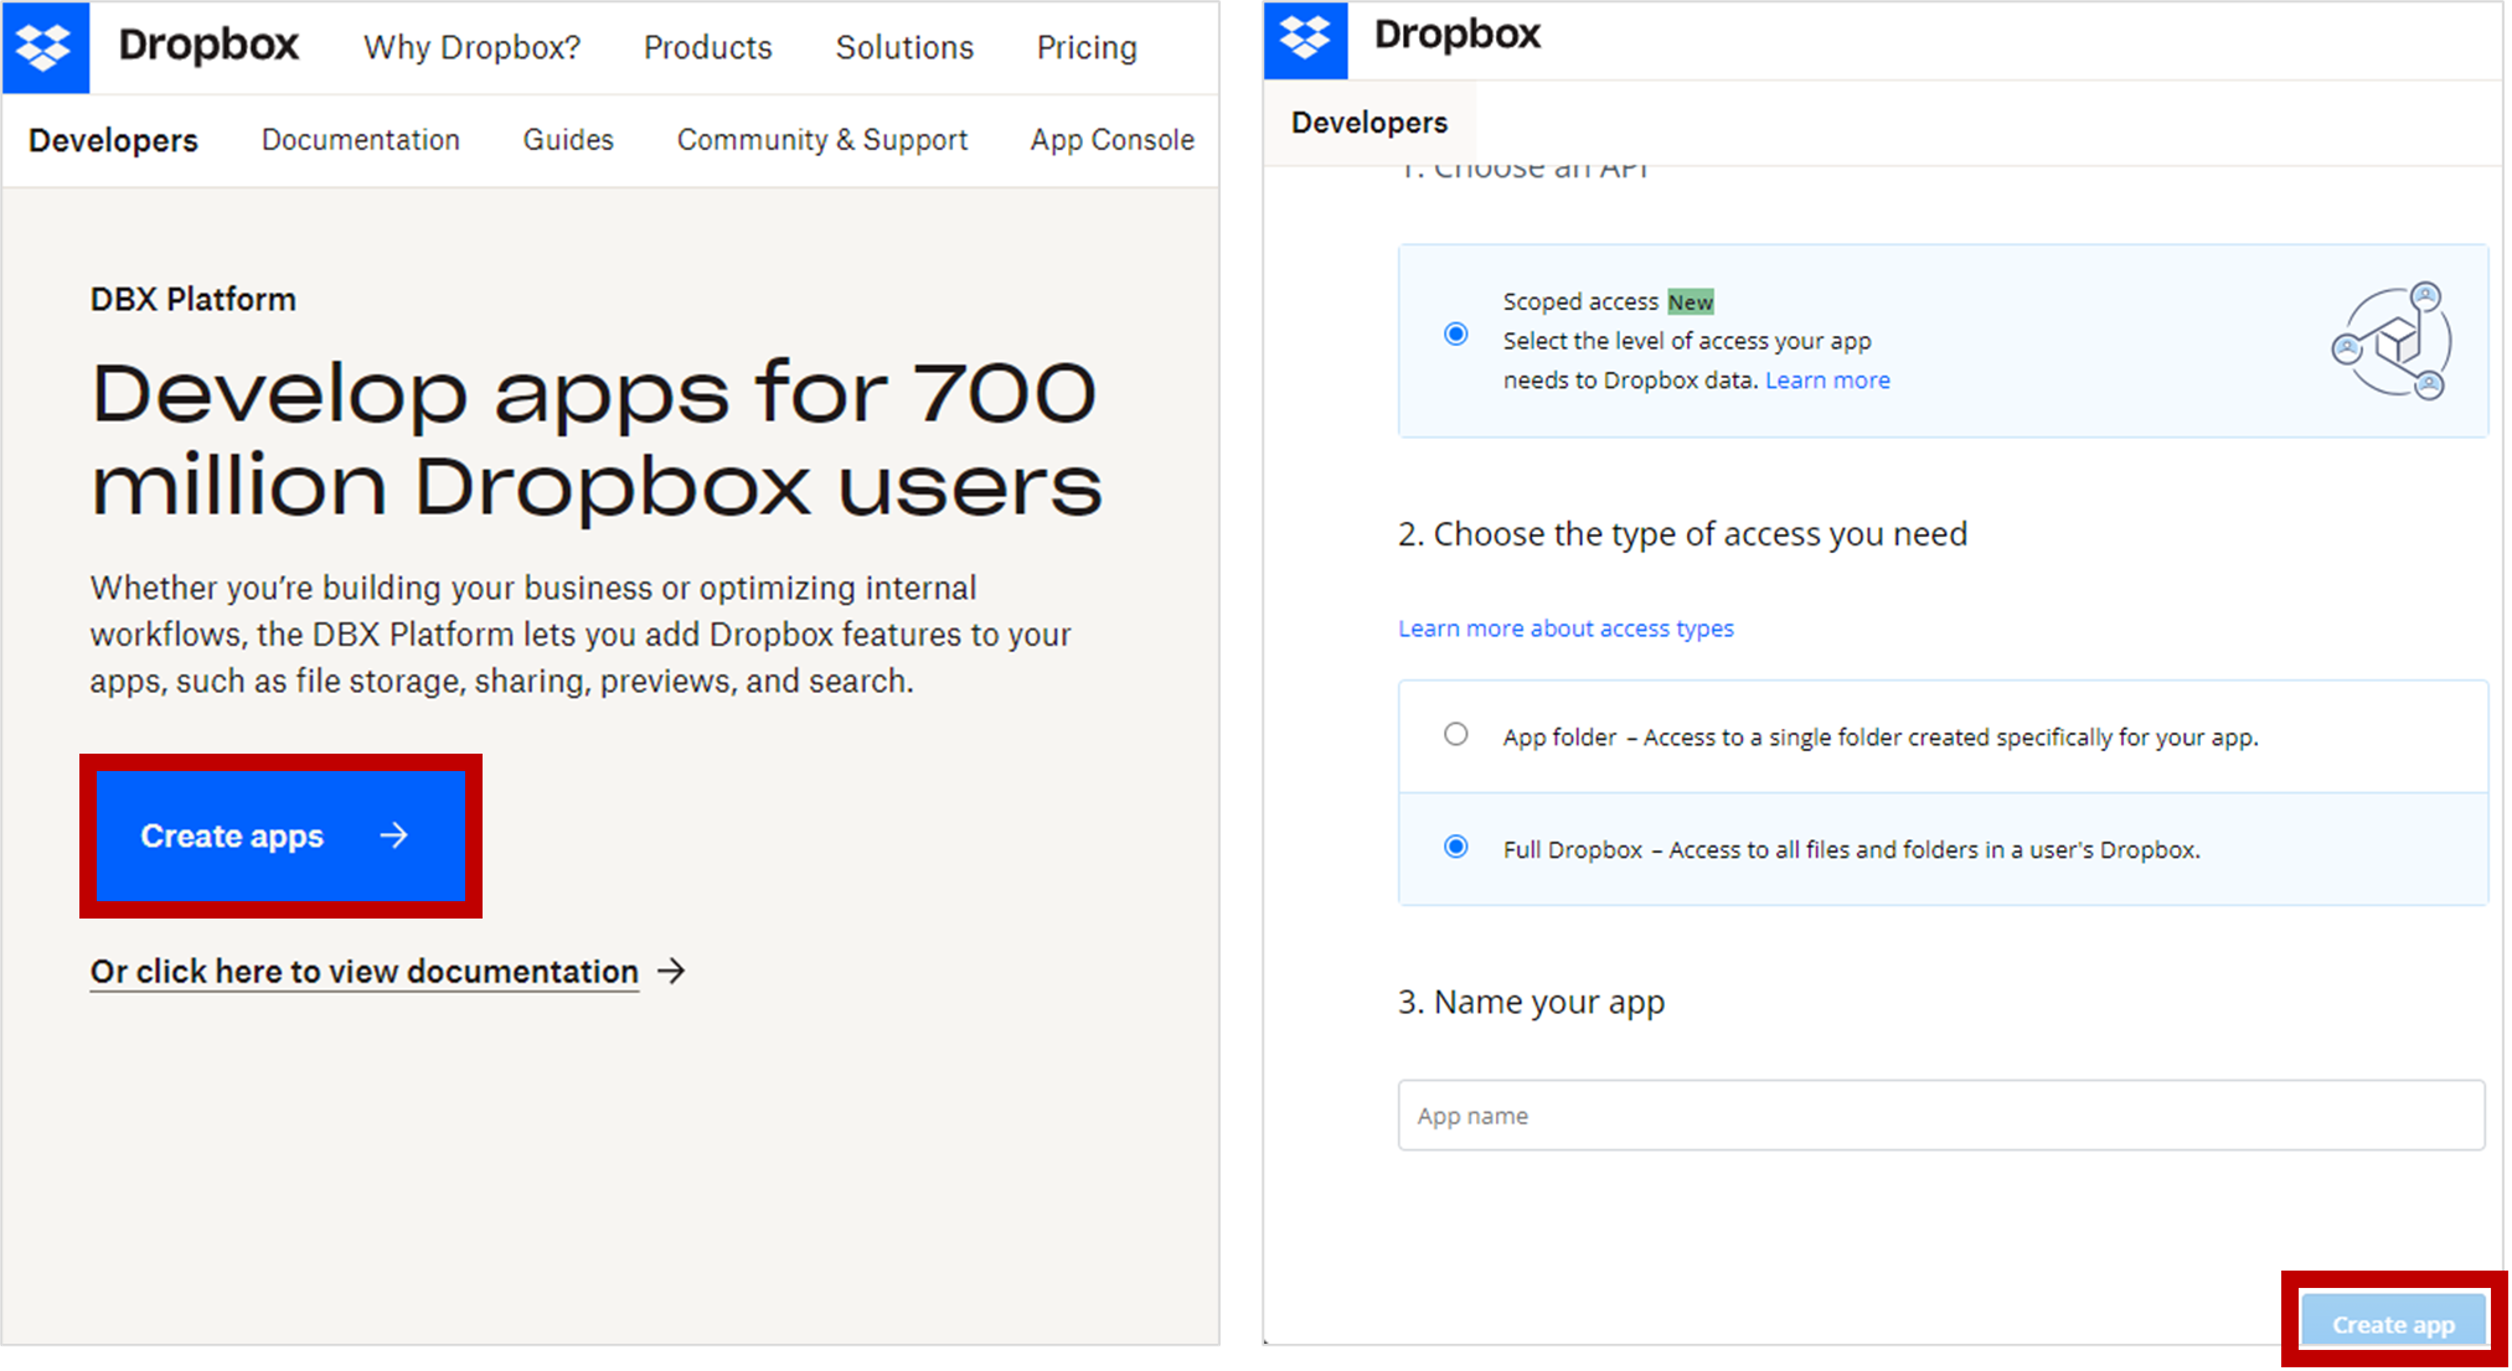
\includegraphics{content/material/ch2/dropbox_create.png}

\subsection{Modify the Permission}\label{modify-the-permission}

Configure your application to permit the viewing and management of files
and folders. In this instance, we've selected all the available options
in the permission settings (for the \textbf{indivisual scope}).

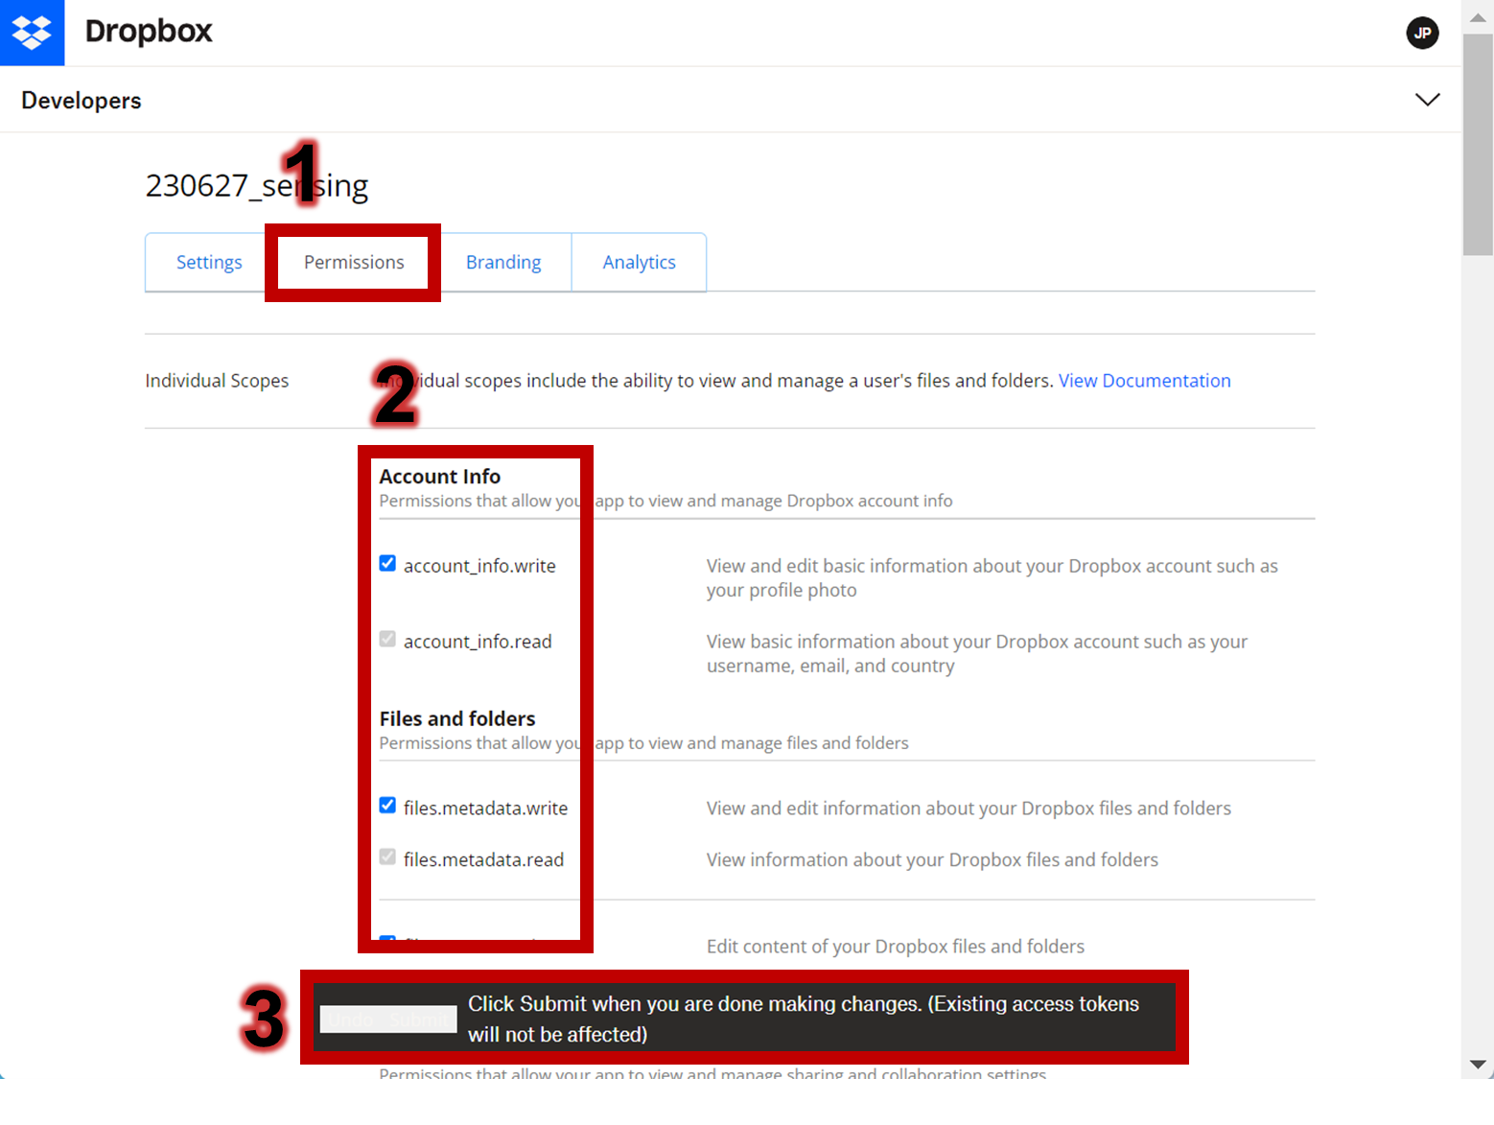
\includegraphics{content/material/ch2/dropbox_permission.png}

\subsection{Install the Necessary
Packages}\label{install-the-necessary-packages}

Switch to a superuser shell session by typing this command:

\begin{Shaded}
\begin{Highlighting}[]
\FunctionTok{sudo}\NormalTok{ su}
\end{Highlighting}
\end{Shaded}

Make sure that curl and git packages are installed on your Pi. You can
do this by entering the following command:

\begin{Shaded}
\begin{Highlighting}[]
\FunctionTok{sudo}\NormalTok{ apt install curl git }\AttributeTok{{-}y}
\end{Highlighting}
\end{Shaded}

\subsection{Install the Dropbox
Uploader}\label{install-the-dropbox-uploader}

Download the
\href{https://github.com/andreafabrizi/Dropbox-Uploader/}{Dropbox
Uploader script} onto your Pi using this command:

\begin{Shaded}
\begin{Highlighting}[]
\FunctionTok{git}\NormalTok{ clone https://github.com/andreafabrizi/Dropbox{-}Uploader.git}
\end{Highlighting}
\end{Shaded}

\subsection{Assign Execution
Permission}\label{assign-execution-permission}

Move into the cloned directory and give the executable permission to the
script by using these commands:

\begin{Shaded}
\begin{Highlighting}[]
\BuiltInTok{cd}\NormalTok{ Dropbox{-}Uploader}
\end{Highlighting}
\end{Shaded}

\begin{Shaded}
\begin{Highlighting}[]
\FunctionTok{sudo}\NormalTok{ chmod +x dropbox\_uploader.sh}
\end{Highlighting}
\end{Shaded}

\subsection{Validate App Permissions on Your
Pi}\label{validate-app-permissions-on-your-pi}

Begin the Dropbox Uploader configuration with the following command:

\begin{Shaded}
\begin{Highlighting}[]
\ExtensionTok{./dropbox\_uploader.sh}
\end{Highlighting}
\end{Shaded}

Enter your app key and app secret in the terminal:

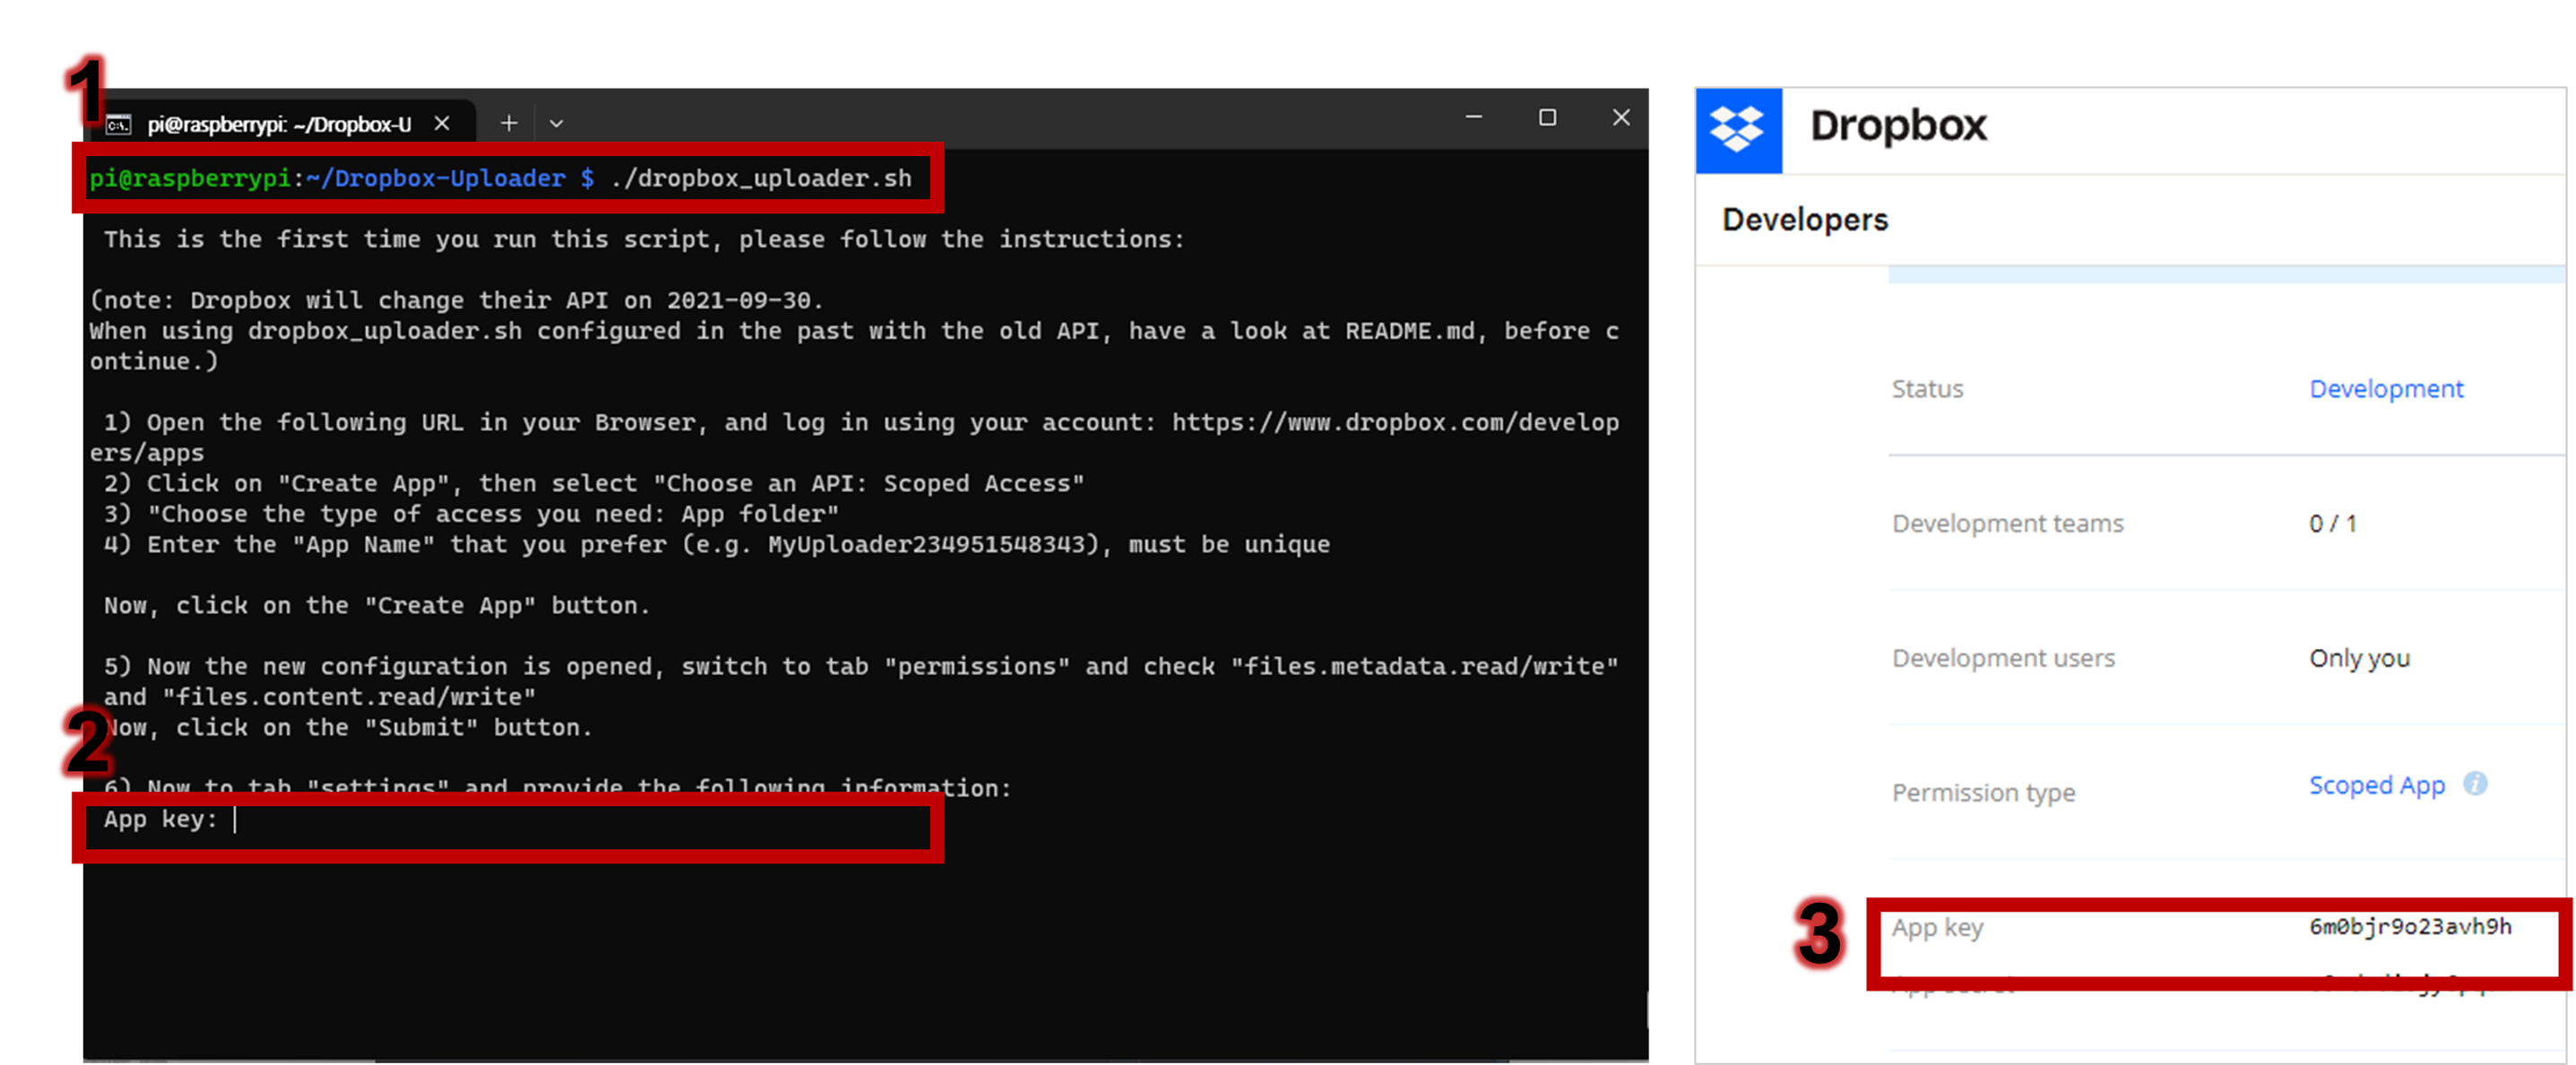
\includegraphics{content/material/ch2/dropbox_register1.png}

Copy and paste the given URL into a web browser, then click `Continue'
and `Allow' to authorize the permissions.

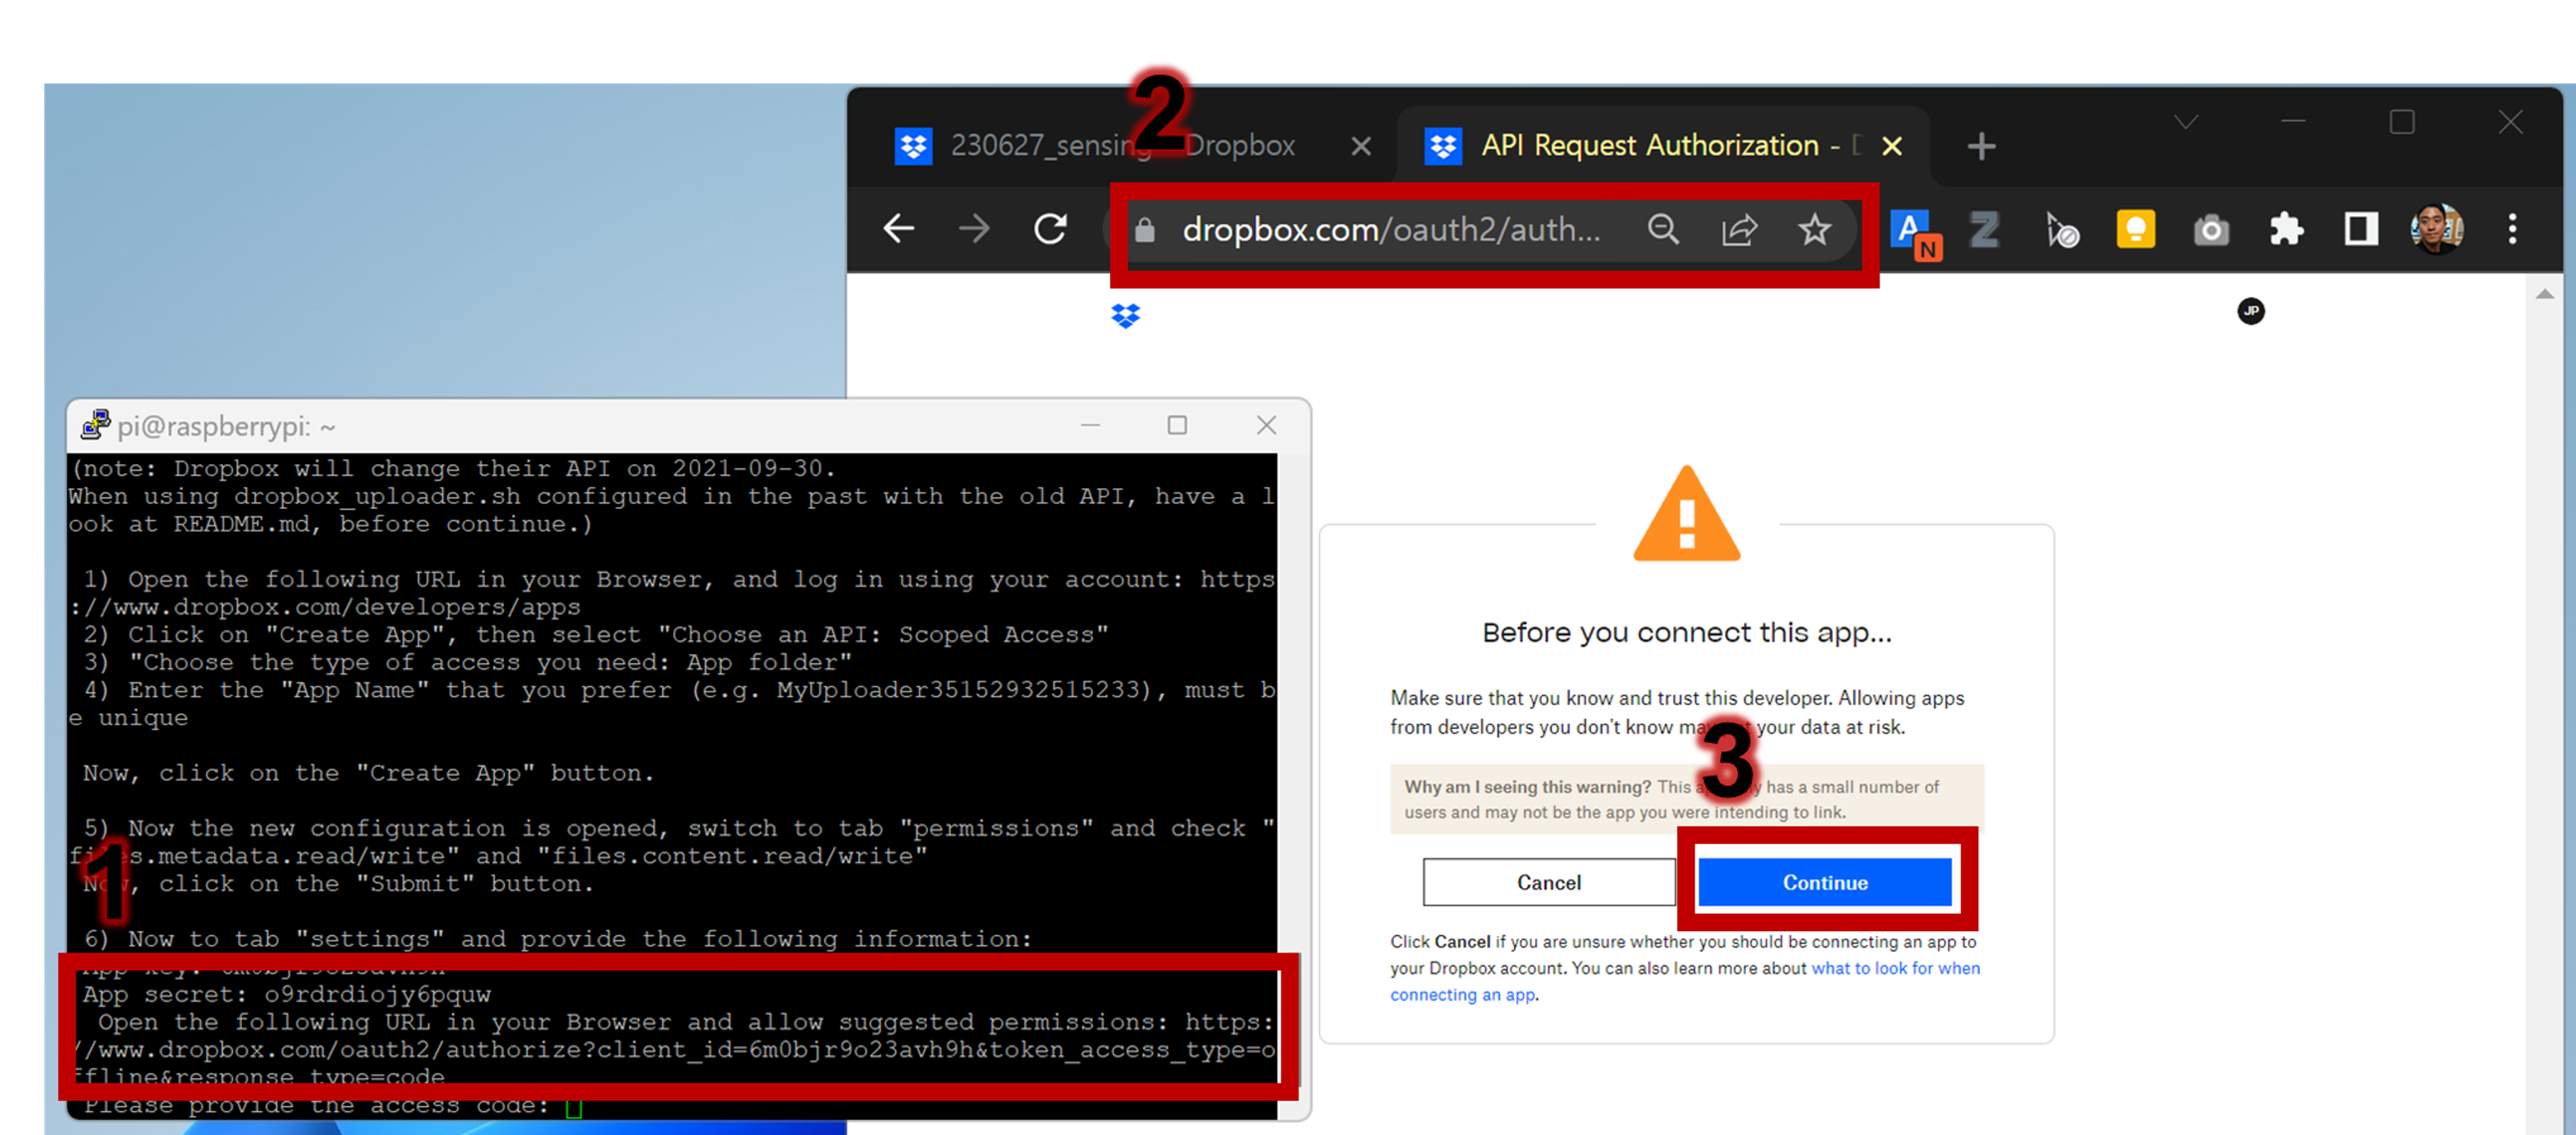
\includegraphics{content/material/ch2/dropbox_register2.png}

Copy and paste the generated access code to the terminal.

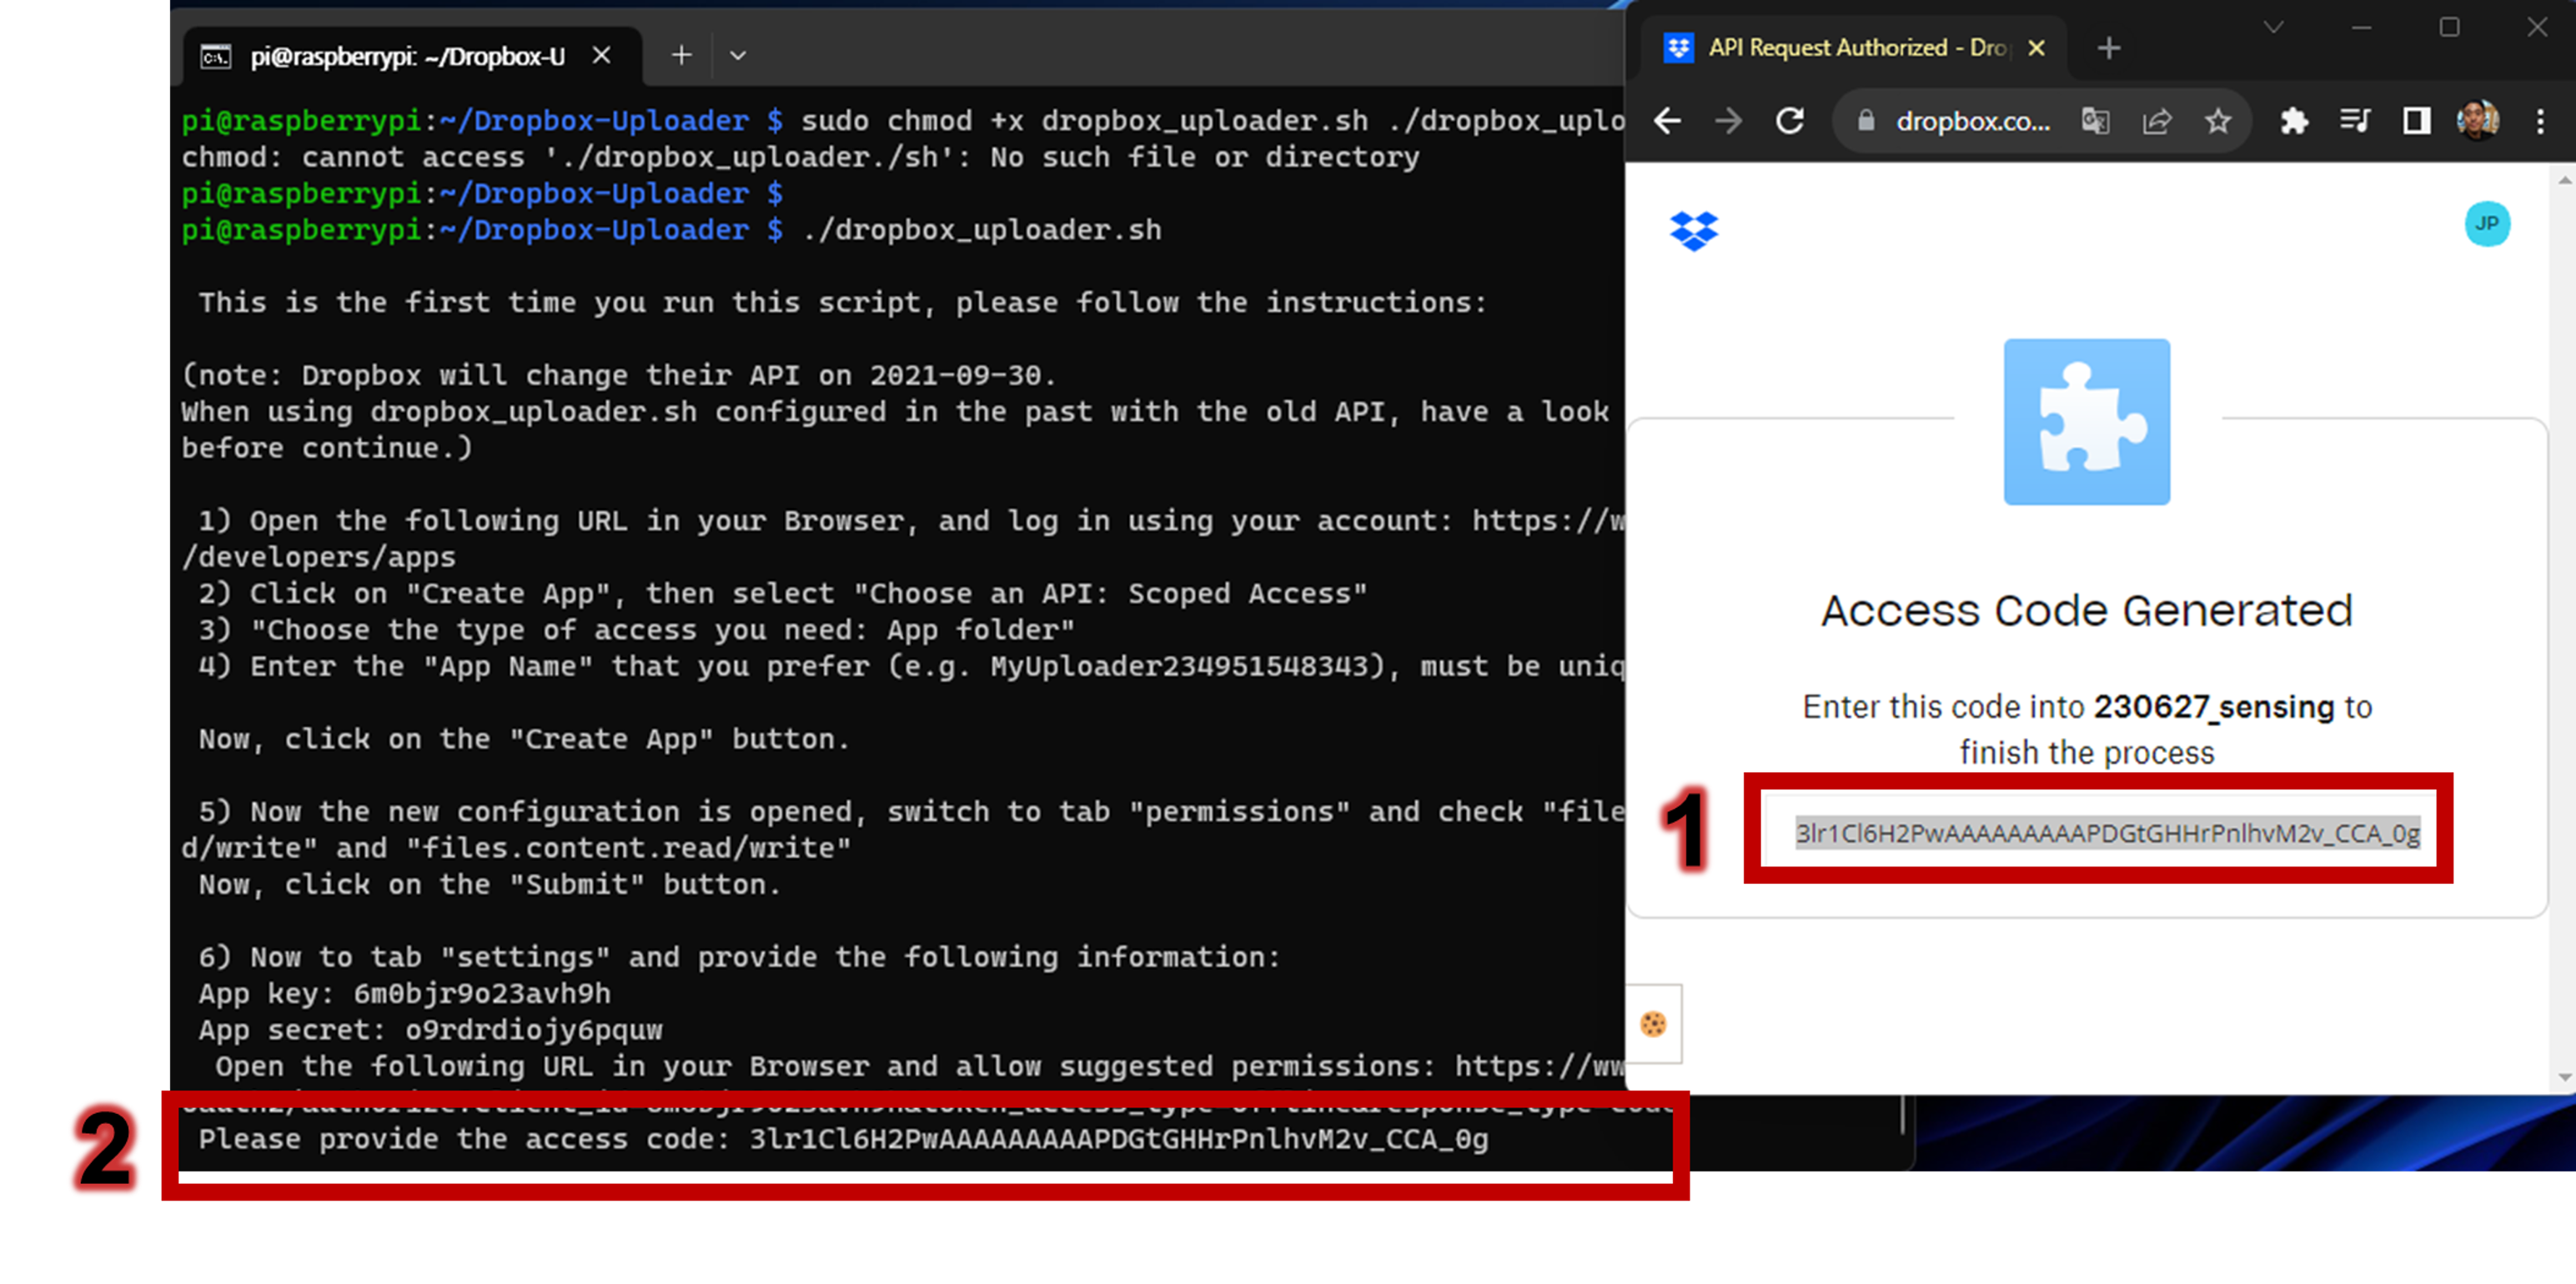
\includegraphics{content/material/ch2/dropbox_register3.png}

\subsection{Verify Cloud Storage
Access}\label{verify-cloud-storage-access}

Employ the upload function to transmit a `README.md' file by executing
this command:

\begin{Shaded}
\begin{Highlighting}[]
\ExtensionTok{./dropbox\_uploader.sh}\NormalTok{ upload README.md /}
\end{Highlighting}
\end{Shaded}

You should be able to view the file that was sent by executing the
command.

\includegraphics{content/material/ch2/test_dropbox_upload.mp4}

Go back to the home directory by executing the command:

\begin{Shaded}
\begin{Highlighting}[]
\BuiltInTok{cd}\NormalTok{ /home/pi}
\end{Highlighting}
\end{Shaded}

\chapter{Sensing Setup}\label{sensing-setup}

This guide walks you through the setup of your Raspberry Pi for urban
sensing. Learn how to fetch essential scripts, install required
packages, and configure settings for optimal sensing performance. Ensure
your device is uniquely identified and ready for data collection.

\section{Getting the Scripts}\label{getting-the-scripts}

Begin by fetching the scripts from the
\href{https://github.com/urbanjuhyeon/urban-sensing-raspi}{urban-sensing-raspi}
GitHub repository.

Ensure you're in the \texttt{/home/pi} directory. If not, navigate there
using:

\begin{Shaded}
\begin{Highlighting}[]
\BuiltInTok{cd}\NormalTok{ /home/pi}
\end{Highlighting}
\end{Shaded}

Clone the repository with:

\begin{Shaded}
\begin{Highlighting}[]
\FunctionTok{git}\NormalTok{ clone https://github.com/urbanjuhyeon/urban{-}sensing{-}raspi.git}
\end{Highlighting}
\end{Shaded}

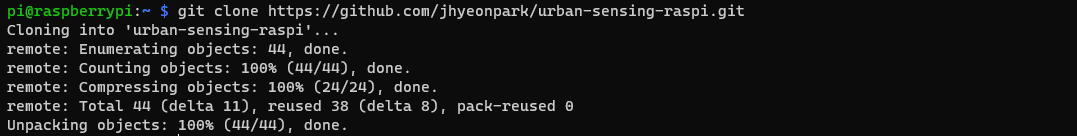
\includegraphics{content/material/ch2/clone_raspi.png}

\subsection*{Repository Overview}\label{repository-overview}
\addcontentsline{toc}{subsection}{Repository Overview}

The repository structure is as follows:

\begin{Shaded}
\begin{Highlighting}[]
\BuiltInTok{.}
\ExtensionTok{├──}\NormalTok{ service.sh}
\ExtensionTok{├──}\NormalTok{ name.sh}
\ExtensionTok{├──}\NormalTok{ envr.sh}
\ExtensionTok{├──}\NormalTok{ packages.sh}
\ExtensionTok{├──}\NormalTok{ code}
\ExtensionTok{│}\NormalTok{   └── start.py}
\ExtensionTok{└──}\NormalTok{ README.md}
\end{Highlighting}
\end{Shaded}

\begin{itemize}
\tightlist
\item
  \texttt{packages.sh}: Handles updates, installations, and other setup
  tasks.
\item
  \texttt{name.sh}: Allows users to set or confirm the unique sensor
  name.
\item
  \texttt{envr.sh}: Configures udev rules and prepares the Pi's
  environment.
\item
  \texttt{service.sh}: Sets up the urban sensing service to launch on
  boot.
\item
  \texttt{start.py}: The main script for the Urban Sensing Service,
  located in `code/default'.
\end{itemize}

\section{Installing Required
Packages}\label{installing-required-packages}

Elevate privileges to a superuser session:

\begin{Shaded}
\begin{Highlighting}[]
\FunctionTok{sudo}\NormalTok{ su}
\end{Highlighting}
\end{Shaded}

Navigate to the repository:

\begin{Shaded}
\begin{Highlighting}[]
\BuiltInTok{cd}\NormalTok{ /home/pi/urban{-}sensing{-}raspi}
\end{Highlighting}
\end{Shaded}

Execute the \texttt{packages.sh} script:

\begin{Shaded}
\begin{Highlighting}[]
\FunctionTok{bash}\NormalTok{ packages.sh}
\end{Highlighting}
\end{Shaded}

\includegraphics{content/material/ch2/bash_packages.mp4}

\section{Setting the Sensor Name}\label{setting-the-sensor-name}

For organized data collection across multiple devices, it's essential to
assign a unique identifier to each sensor. This segment aids you in
naming your Raspberry Pi sensor and integrating it into a Python script.

Navigate to the repository:

\begin{Shaded}
\begin{Highlighting}[]
\BuiltInTok{cd}\NormalTok{ /home/pi/urban{-}sensing{-}raspi}
\end{Highlighting}
\end{Shaded}

Run the \texttt{name.sh} script. If no name is provided, the default
(\texttt{raspberrypi}) will be applied:

\begin{Shaded}
\begin{Highlighting}[]
\FunctionTok{bash}\NormalTok{ name.sh}
\end{Highlighting}
\end{Shaded}

Post this, the sensor name can be retrieved from the
\texttt{sensor\_name.conf} file for usage.

\includegraphics{content/material/ch2/bash_naming.mp4}

\section{Configuring Settings}\label{configuring-settings}

Configure the Raspberry Pi to set its internal WiFi to \texttt{wlan0}.
When you connect an external adapter, it will be assigned differently.
To determine the MAC address of the internal WiFi, execute the following
command:

\begin{Shaded}
\begin{Highlighting}[]
\ExtensionTok{ifconfig}
\end{Highlighting}
\end{Shaded}

In my setup, the WiFi with the MAC address \texttt{b8:27:eb:0c:70:38}
was assigned to \texttt{wlan0}, while the external adapter received a
different assignment.

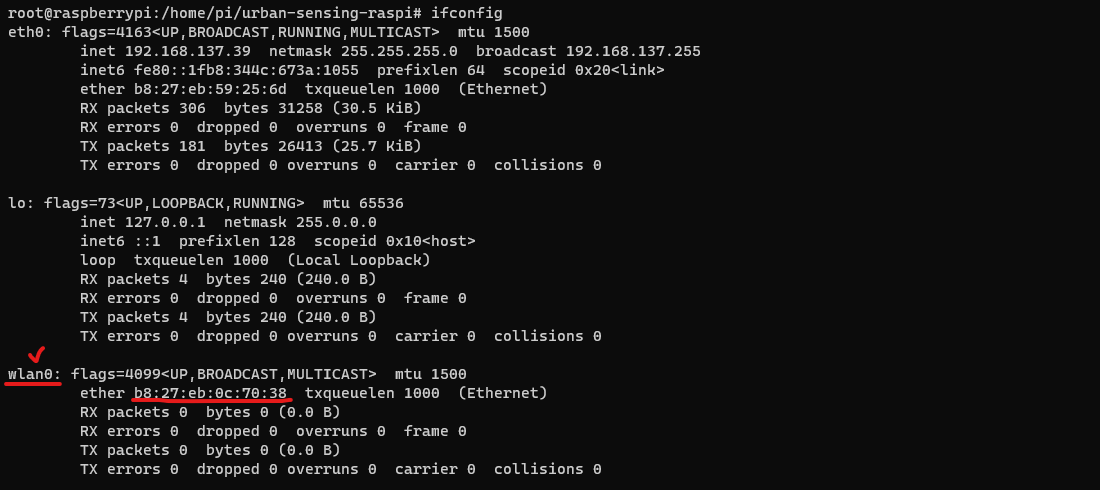
\includegraphics{content/material/ch2/ifconfig_wlan0.png}

Navigate to the repository:

\begin{Shaded}
\begin{Highlighting}[]
\BuiltInTok{cd}\NormalTok{ /home/pi/urban{-}sensing{-}raspi}
\end{Highlighting}
\end{Shaded}

Run the \texttt{envr.sh} script:

\begin{Shaded}
\begin{Highlighting}[]
\FunctionTok{bash}\NormalTok{ envr.sh}
\end{Highlighting}
\end{Shaded}

This script ensures consistent network interface naming with udev rules
at boot.

\includegraphics{content/material/ch2/bash_envr.mp4}

\chapter{Implementation}\label{implementation}

Dive into the step-by-step process of implementing and testing the Urban
Sensing Service on your Raspberry Pi, both in a controlled environment
\emph{(6.1)} and in real-world scenarios \emph{(6.2)}.

\section{Sensing Service Testing in Controlled
Environment}\label{sensing-service-testing-in-controlled-environment}

\subsection{Raspberry Pi Setup}\label{raspberry-pi-setup-1}

Before setting up, power off the Raspberry Pi. Once turned off, insert
the additional WiFi adapter. Afterward, power the Raspberry Pi back on.

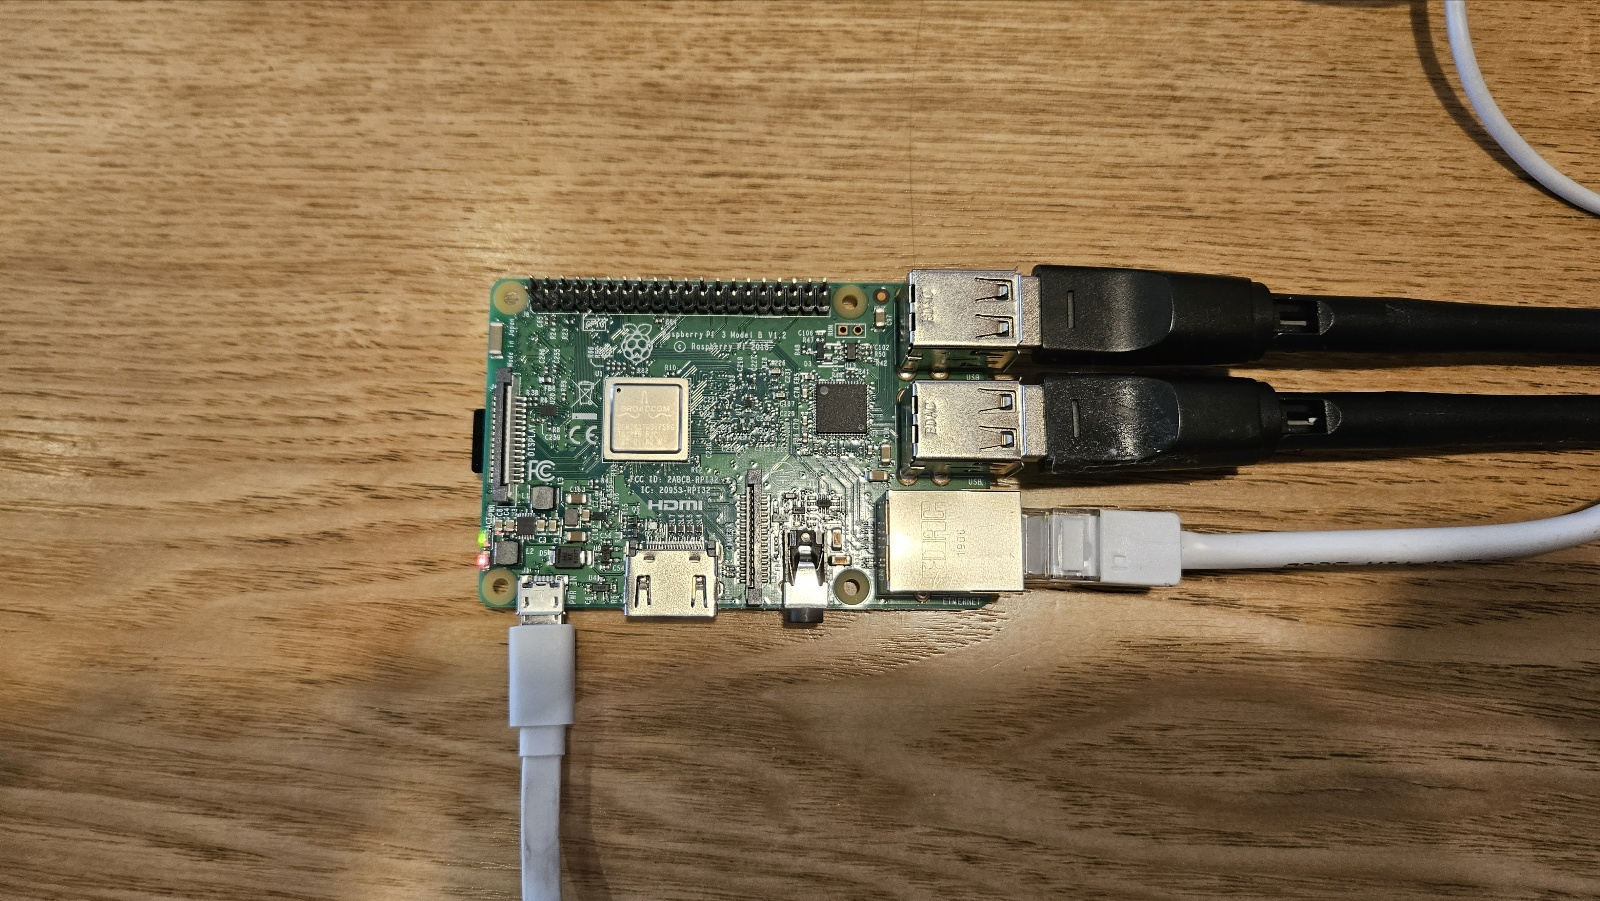
\includegraphics{content/material/ch2/pi_plugged.jpg}

Access the Raspberry Pi via ssh and check the wlan interface to check
the internal wifi set to be wlan0 by excueting this:

\begin{Shaded}
\begin{Highlighting}[]
\ExtensionTok{ifconfig}
\end{Highlighting}
\end{Shaded}

Ensure that the \texttt{wlan0} interface is correctly assigned. The
internal interface should have a MAC address starting with
\texttt{b8:27:eb}. Subsequent WiFi adapters should follow a sequence
like \texttt{wlan1}, \texttt{wlan2}, and so on.

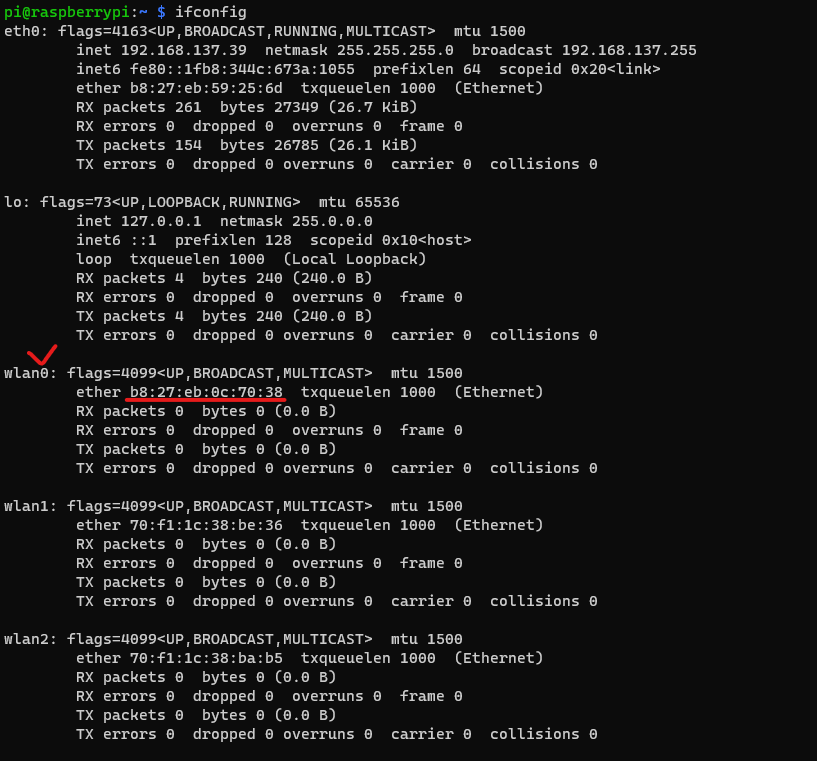
\includegraphics[width=0.5\textwidth,height=\textheight]{content/material/ch2/ifconfig_wlan_check.png}

If the assignment isn't correct, refer to Section 2.4 for the
appropriate setup instructions.

\subsection{Script Execution}\label{script-execution}

Easily access the superuser shell with:

\begin{Shaded}
\begin{Highlighting}[]
\FunctionTok{sudo}\NormalTok{ su}
\end{Highlighting}
\end{Shaded}

Initiate the Urban Sensing code:

\begin{Shaded}
\begin{Highlighting}[]
\ExtensionTok{python3}\NormalTok{ urban{-}sensing{-}raspi/code/start.py}
\end{Highlighting}
\end{Shaded}

Let it run for about 2 minutes before halting it using \texttt{Ctrl+C}.

\includegraphics{content/material/ch2/run_script.mp4}

\subsection{Customizing Your Sensing}\label{customizing-your-sensing}

The Urban Sensing Service isn't just about standard WiFi data
collection; it offers a broader scope:

\begin{itemize}
\item
  \textbf{Retain Raw WiFi Packets} : Use the \texttt{-i} option:

\begin{Shaded}
\begin{Highlighting}[]
\ExtensionTok{python3}\NormalTok{ urban{-}sensing{-}raspi/code/start.py }\AttributeTok{{-}i}
\end{Highlighting}
\end{Shaded}
\item
  \textbf{Introduce Bluetooth Sensing} : Add the \texttt{-b} option:

\begin{Shaded}
\begin{Highlighting}[]
\ExtensionTok{python3}\NormalTok{ urban{-}sensing{-}raspi/code/start.py }\AttributeTok{{-}b}
\end{Highlighting}
\end{Shaded}
\item
  \textbf{Discover More Options} : Read our the
  \href{https://github.com/urbanjuhyeon/urban-sensing-raspi}{GitHub
  Repository}.
\end{itemize}

\section{Verifying the Results}\label{verifying-the-results}

\textbf{1. Access the Pi folder:} type
\texttt{\textbackslash{}\textbackslash{}raspberrypi\textbackslash{}share}
on file explore.

\textbf{2. Look around `stats' Folder} :

\begin{itemize}
\tightlist
\item
  Verify that file names reflect the exact execution time.
\item
  Confirm files have been transferred to Dropbox Storage.
\end{itemize}

\includegraphics{content/material/ch2/verify_result_1.mp4}

\textbf{3. `data' Folder} :

\begin{itemize}
\tightlist
\item
  If you used \texttt{-b}, expect a Bluetooth file. Otherwise, it won't
  appear.
\item
  Check for the creation of the WiFi packet file. To delve deeper, use
  \href{https://sqlitebrowser.org/}{DB Browser for SQLite}.
\end{itemize}

\includegraphics{content/material/ch2/verify_result_2.mp4}

\section{Setting Up Sensing Service}\label{setting-up-sensing-service}

Once you've validated the sensing outputs, you can finalize the settings
to fit your objectives. Notably, this will allow your Raspberry Pi to
initiate the sensing service upon booting up.

Execute the following script:

\begin{Shaded}
\begin{Highlighting}[]
\FunctionTok{bash}\NormalTok{ urban{-}sensing{-}raspi/service.sh}
\end{Highlighting}
\end{Shaded}

Follow the on-screen prompts and ensure its proper functioning. Exit the
status info using \texttt{ctrl+c}.

\includegraphics{content/material/ch2/bash_service.mp4}

\begin{tcolorbox}[enhanced jigsaw, opacityback=0, colbacktitle=quarto-callout-note-color!10!white, toptitle=1mm, colframe=quarto-callout-note-color-frame, rightrule=.15mm, title=\textcolor{quarto-callout-note-color}{\faInfo}\hspace{0.5em}{Note}, toprule=.15mm, colback=white, bottomrule=.15mm, coltitle=black, breakable, leftrule=.75mm, left=2mm, opacitybacktitle=0.6, bottomtitle=1mm, arc=.35mm, titlerule=0mm]

After running service.sh, your Raspberry Pi will start start.py on every
boot. If you need to do tasks like file transfers, pause this service.
The start.py has a 30-second delay at the start. If you stop the service
within this time using \texttt{systemctl\ stop\ sensing.service}, the
script won't perform any actions.

\begin{Shaded}
\begin{Highlighting}[]
\FunctionTok{sudo}\NormalTok{ systemctl stop sensing.service}
\end{Highlighting}
\end{Shaded}

\end{tcolorbox}

\section{Sensing Service Testing in Real-world
Scenarios}\label{sensing-service-testing-in-real-world-scenarios}

In this section, we'll test the sensing service without Ethernet,
simulating a real-world application. Follow these detailed steps for a
successful setup and operation:

\subsection{Activate Mobile Hotspot}\label{activate-mobile-hotspot}

Activate the hotspot on your mobile device. This is essential for
providing internet connectivity to the Raspberry Pi, which will enable
time synchronization and status updates via Dropbox.

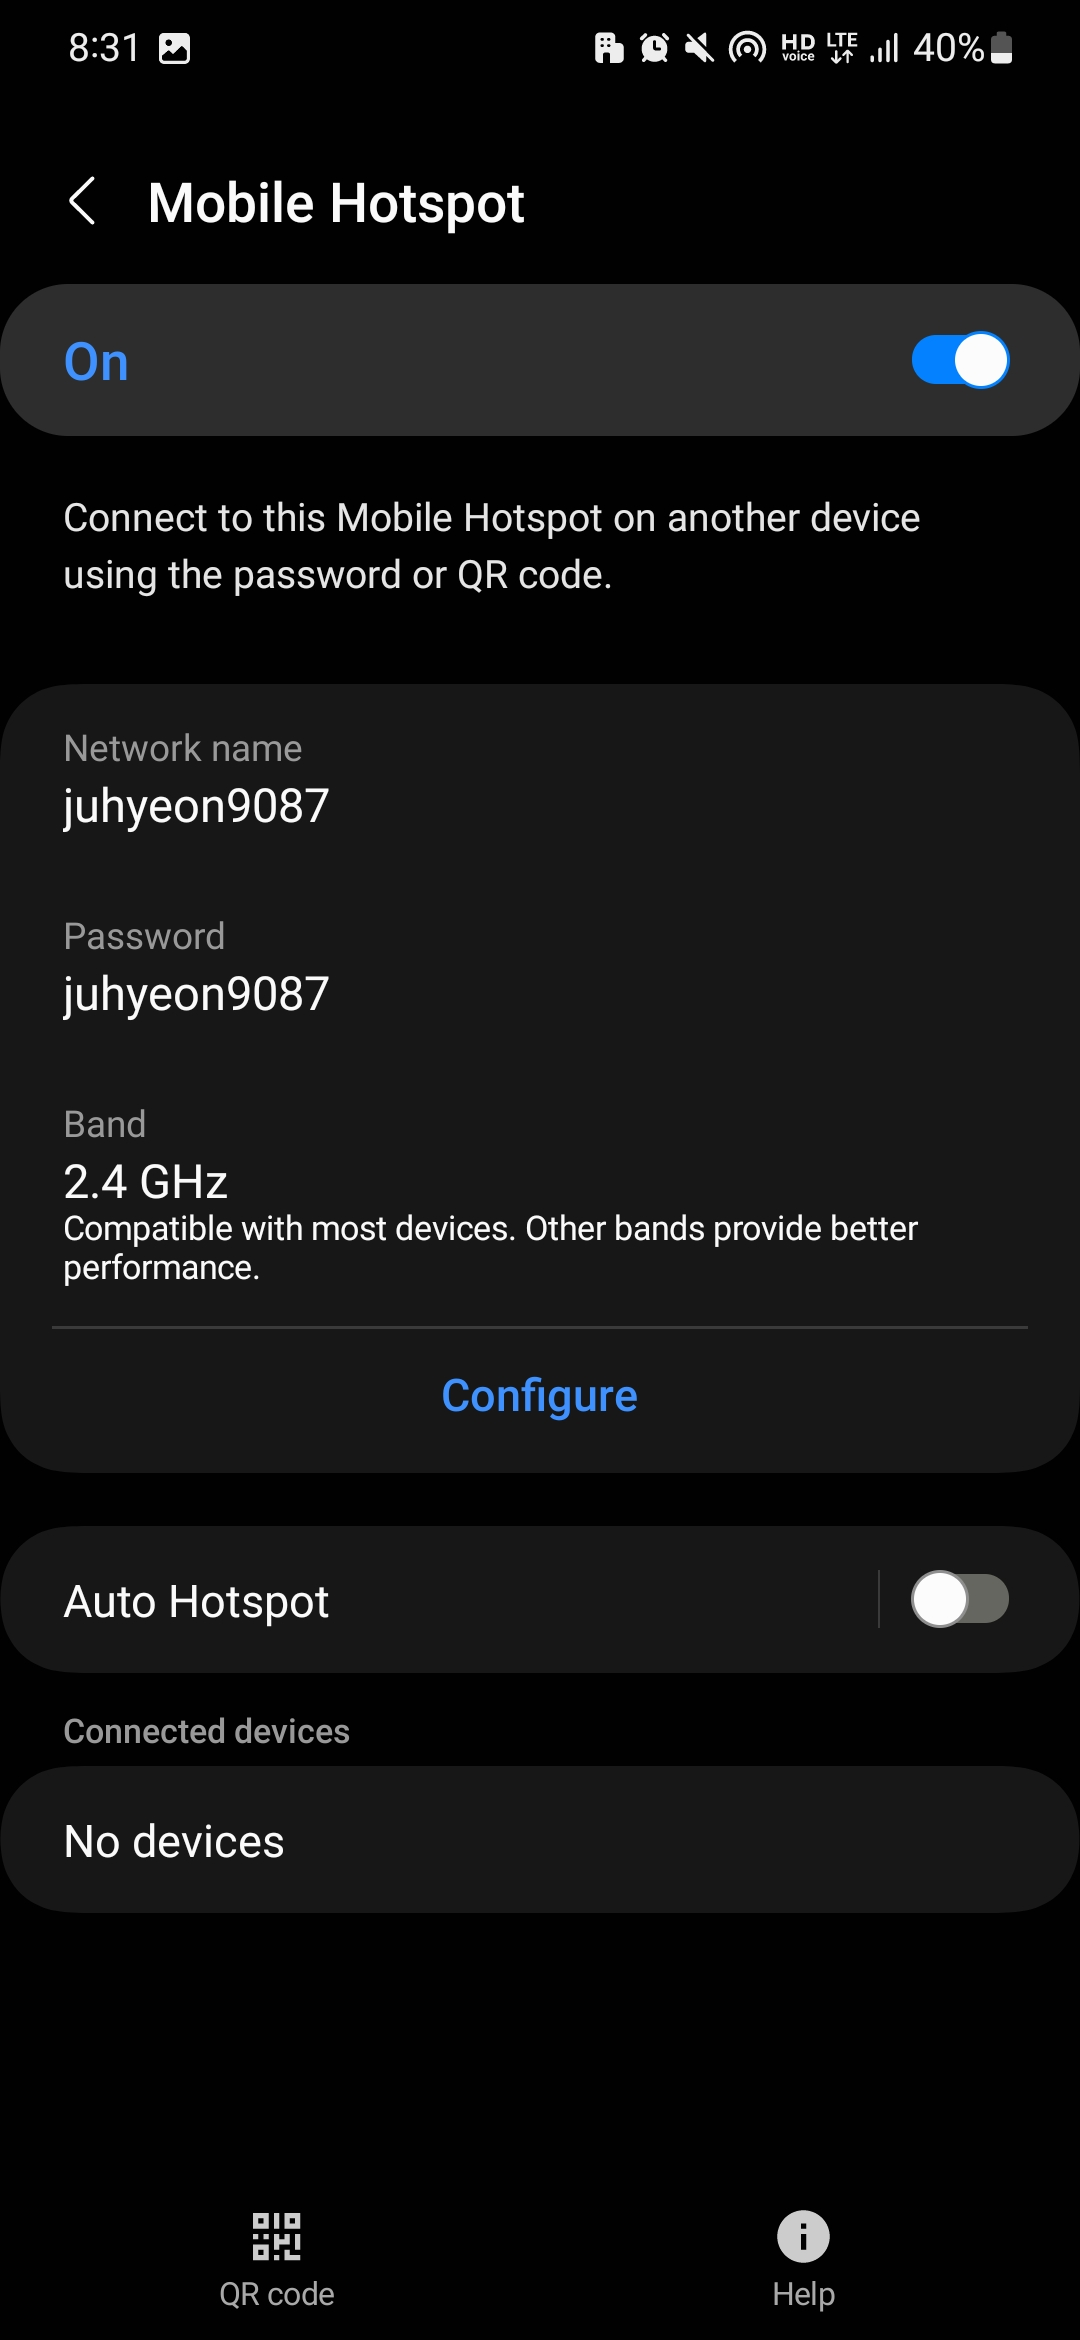
\includegraphics[width=0.5\textwidth,height=\textheight]{content/material/ch2/turnon_hotspot.jpg}

\subsection{Connect the External
Battery}\label{connect-the-external-battery}

Ensure you've connected an external battery to power both your Raspberry
Pi and the WiFi adapters.

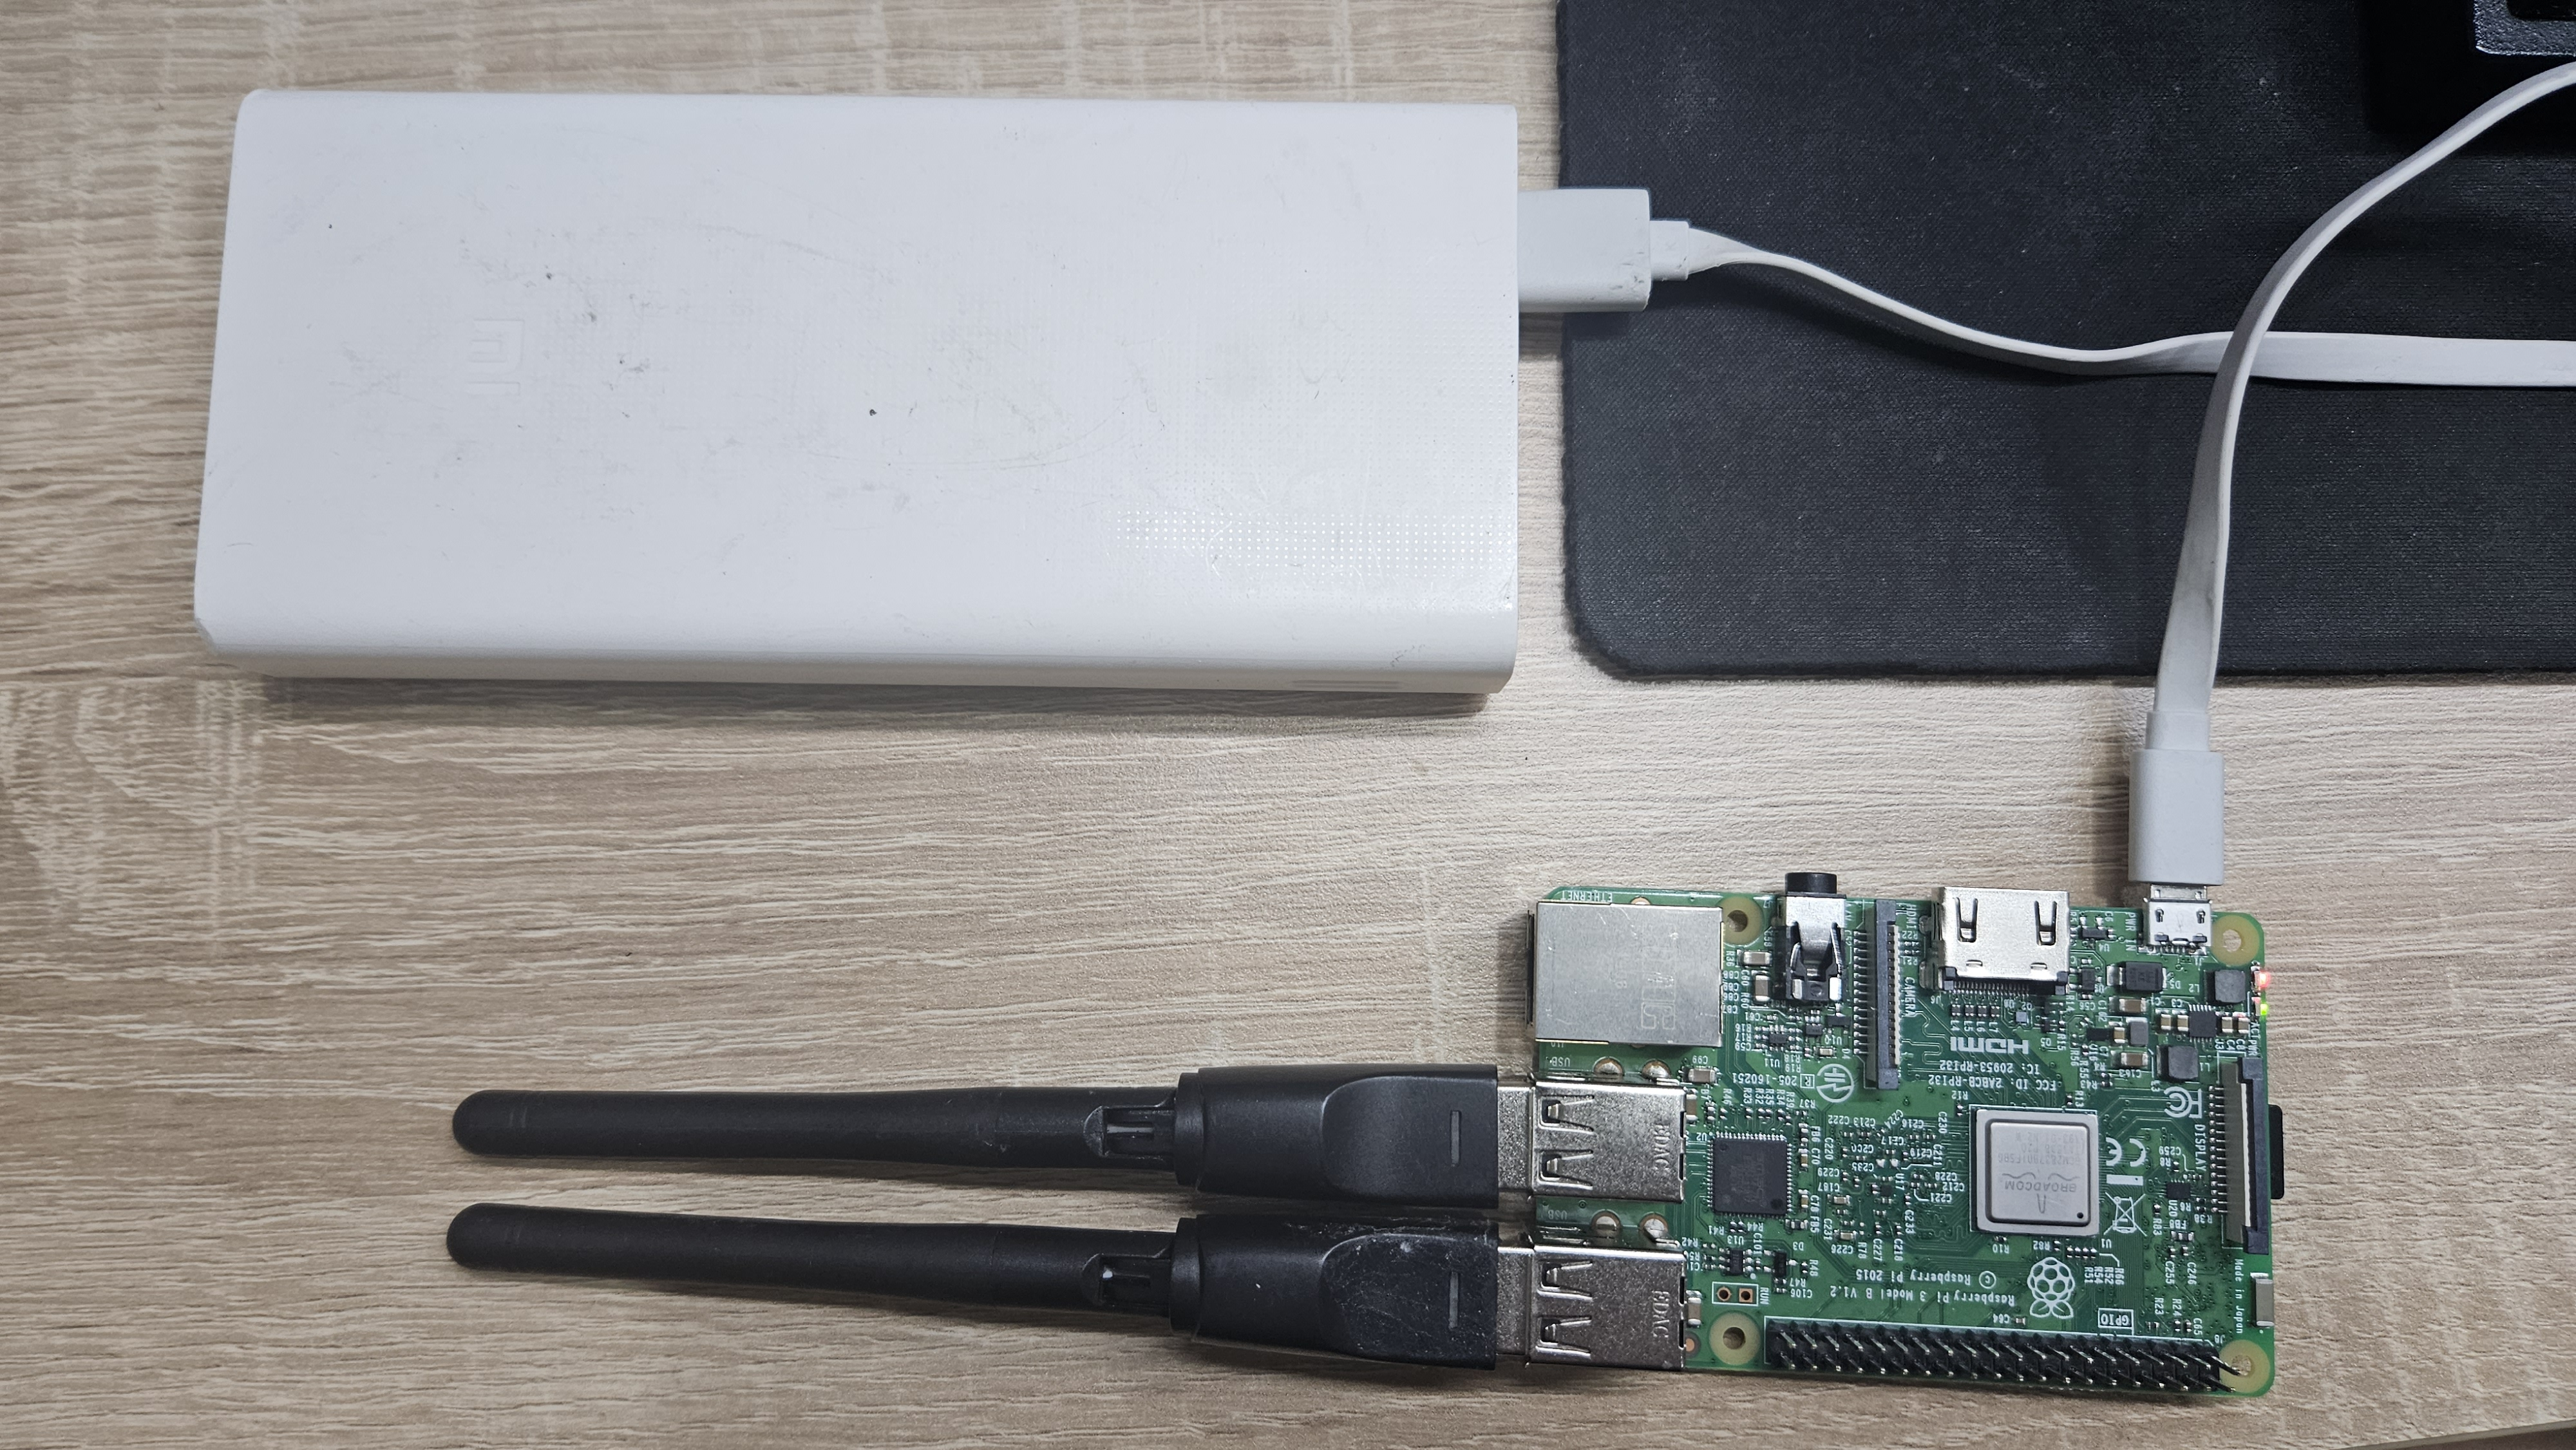
\includegraphics{content/material/ch2/plug_external.jpg}

\subsection{Monitor WiFi Adapter
Activity}\label{monitor-wifi-adapter-activity}

Check for indicator lights on the WiFi adapter. In station mode, when
the adapter is networking, the lights should turn on. You should also
see the Raspberry Pi appear on your mobile hotspot interface.

\begin{tcolorbox}[enhanced jigsaw, opacityback=0, colbacktitle=quarto-callout-note-color!10!white, toptitle=1mm, colframe=quarto-callout-note-color-frame, rightrule=.15mm, title=\textcolor{quarto-callout-note-color}{\faInfo}\hspace{0.5em}{Note}, toprule=.15mm, colback=white, bottomrule=.15mm, coltitle=black, breakable, leftrule=.75mm, left=2mm, opacitybacktitle=0.6, bottomtitle=1mm, arc=.35mm, titlerule=0mm]

If the status lights remain off or the Raspberry Pi does not appear on
your hotspot interface, there might be an issue with your adapter.
Consider getting a replacement.

\end{tcolorbox}

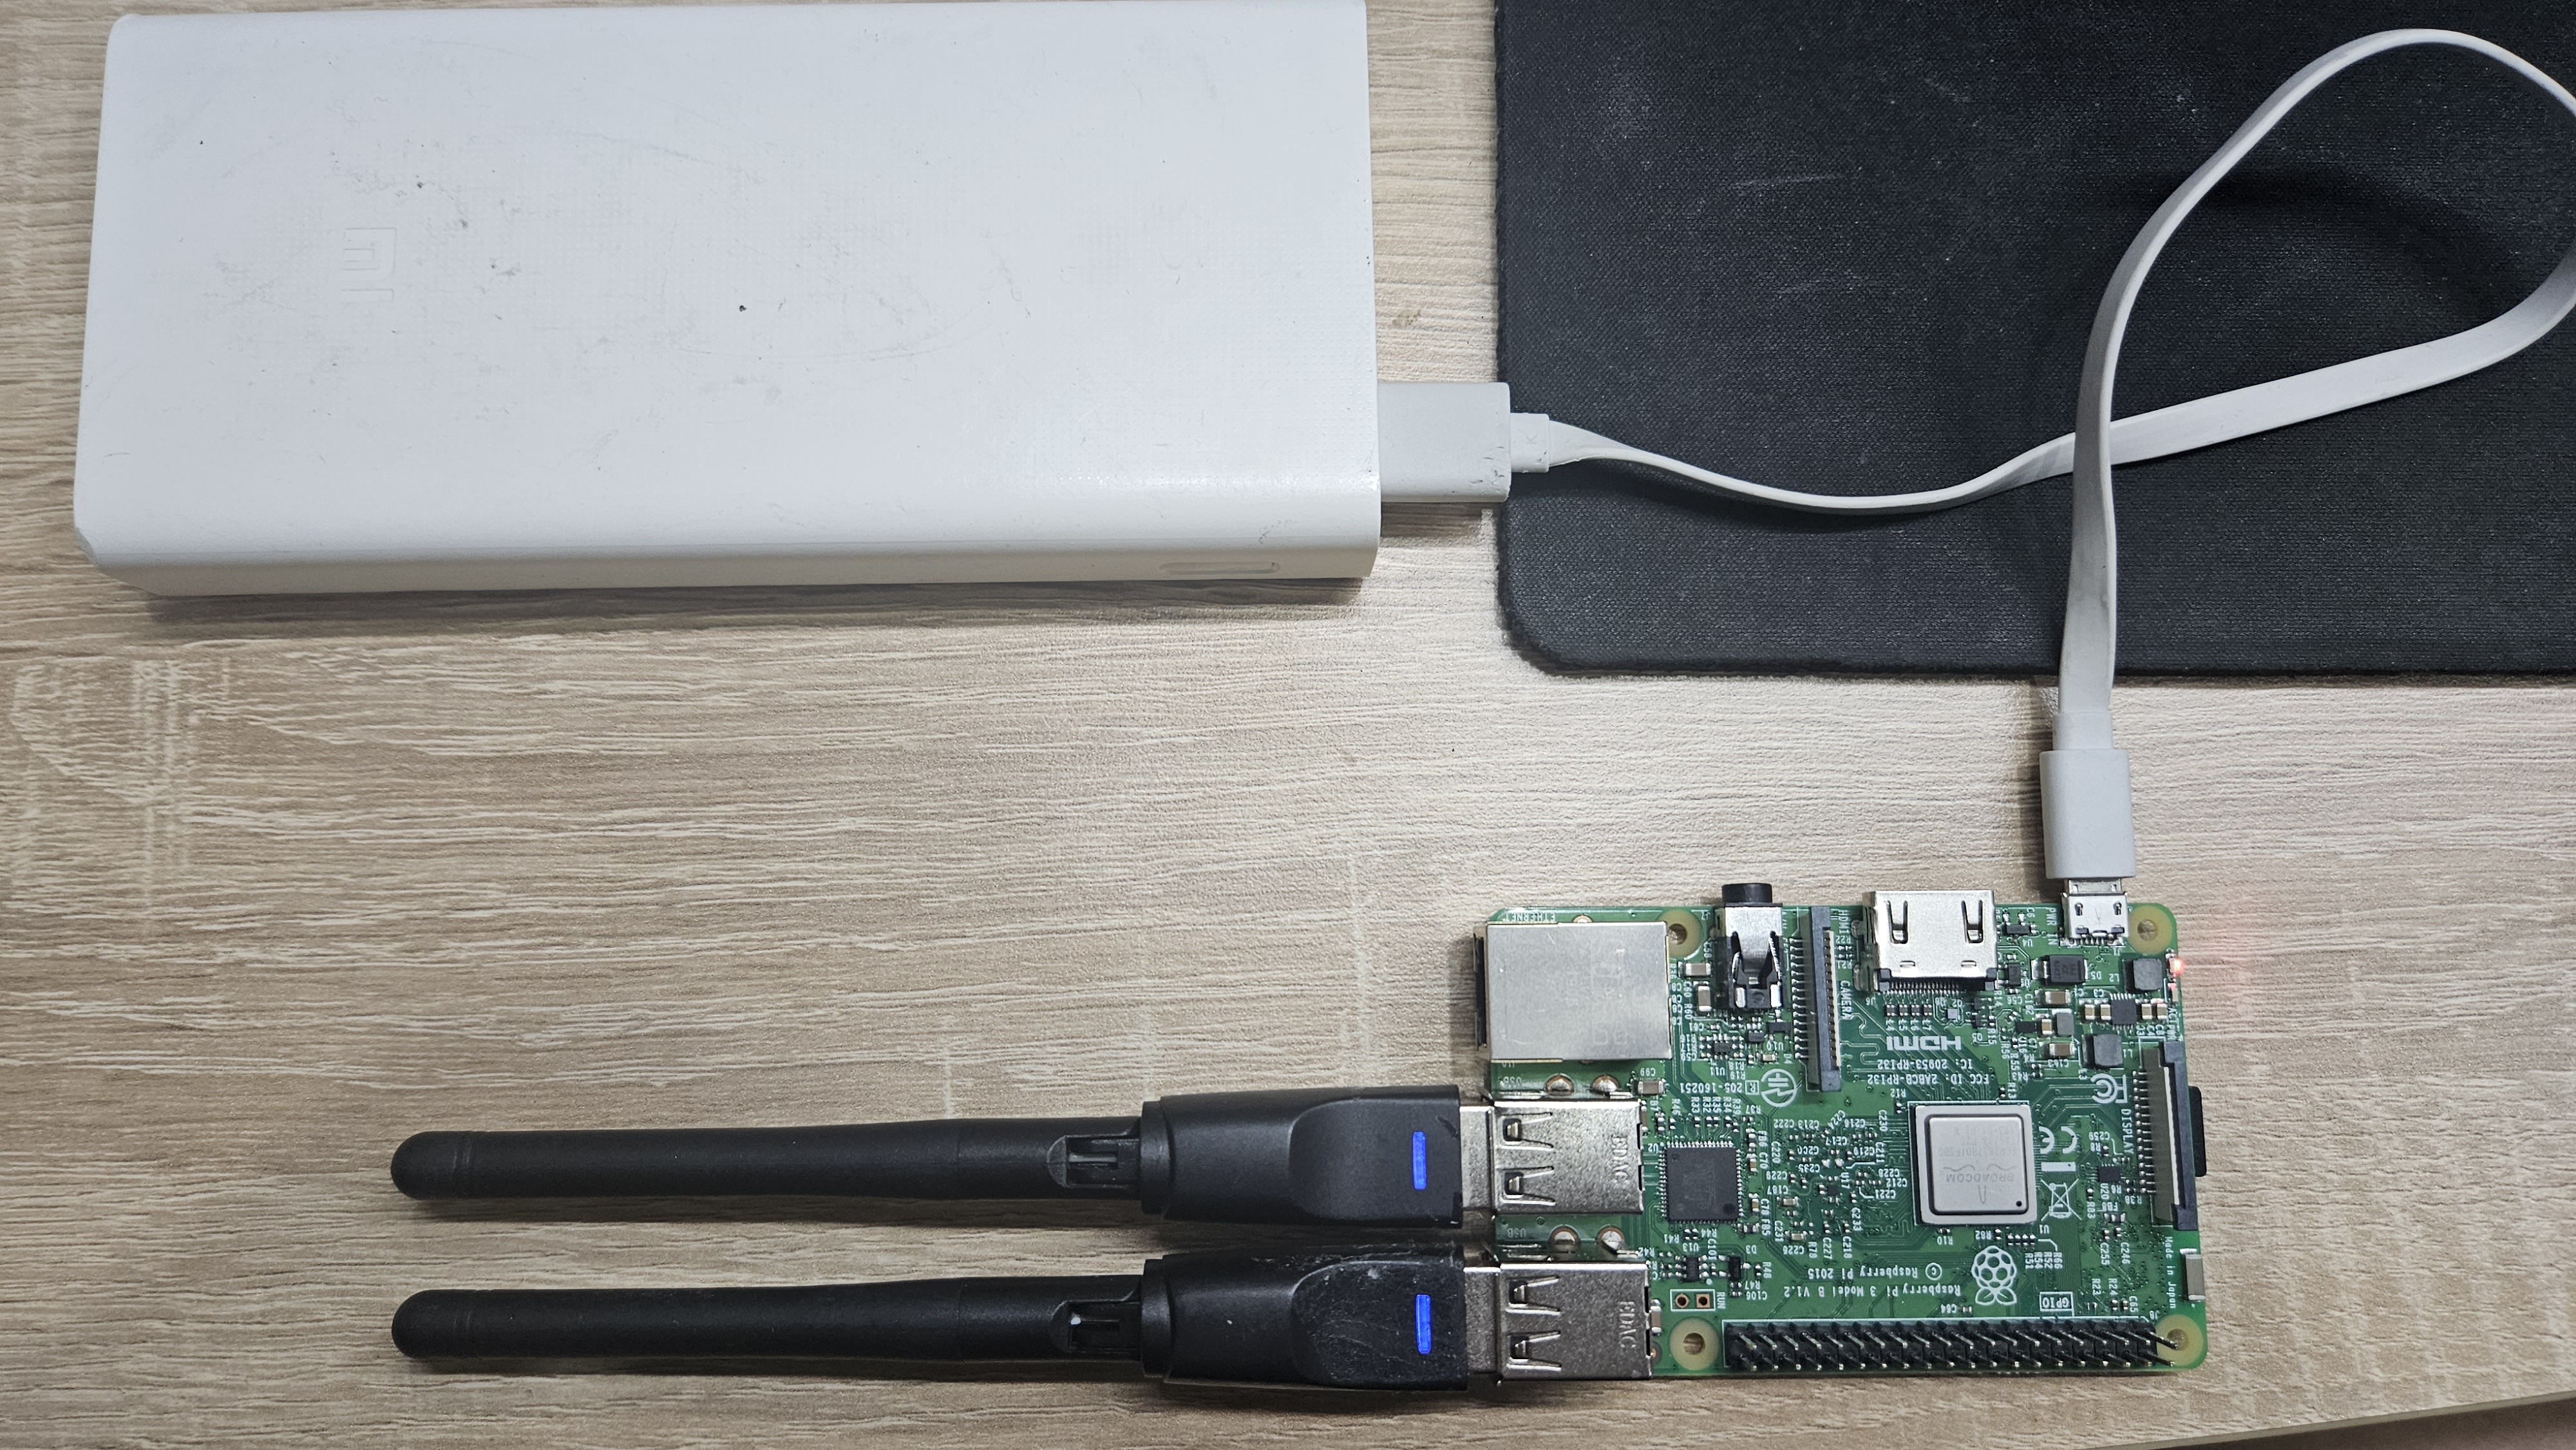
\includegraphics{content/material/ch2/adapter_light.jpg}

Observe the WiFi adapter's status lights. When networked (station mode),
these should illuminate. Concurrently, you'll see the Raspberry Pi
connect to your mobile hotspot interface.

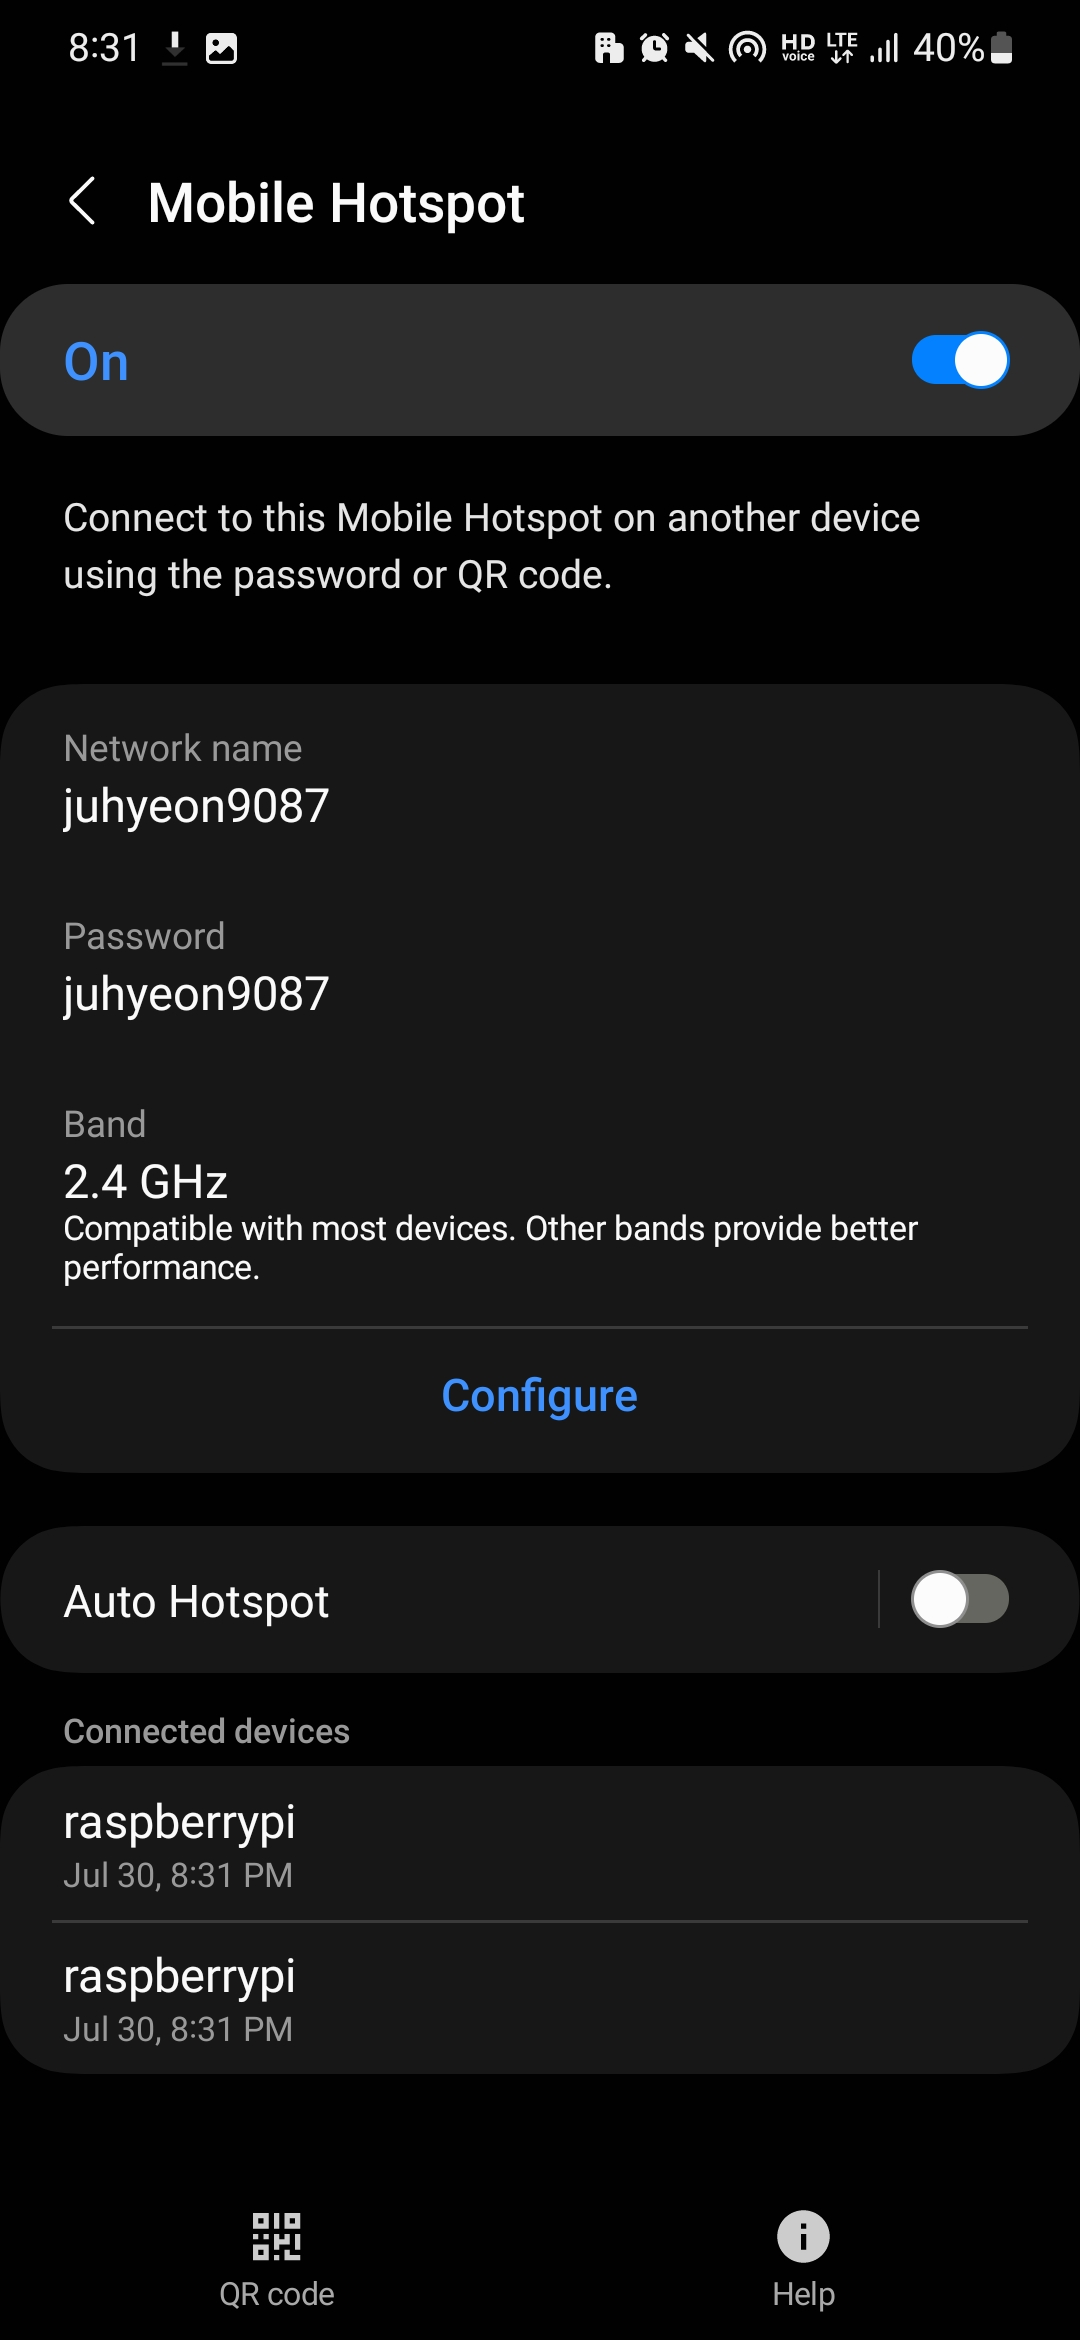
\includegraphics[width=0.5\textwidth,height=\textheight]{content/material/ch2/check_hotspot.jpg}

\begin{tcolorbox}[enhanced jigsaw, opacityback=0, colbacktitle=quarto-callout-note-color!10!white, toptitle=1mm, colframe=quarto-callout-note-color-frame, rightrule=.15mm, title=\textcolor{quarto-callout-note-color}{\faInfo}\hspace{0.5em}{Note}, toprule=.15mm, colback=white, bottomrule=.15mm, coltitle=black, breakable, leftrule=.75mm, left=2mm, opacitybacktitle=0.6, bottomtitle=1mm, arc=.35mm, titlerule=0mm]

When accessing your Raspberry Pi via a mobile phone, the
\texttt{raspberrypi} network might not disappear immediately. This is
attributed to the \texttt{wlan0} interface. A Python script will
disconnect and turn off the \texttt{wlan0} function approximately 3
minutes later.

\end{tcolorbox}

\subsection{Validate Dropbox
Connectivity}\label{validate-dropbox-connectivity}

Once connected to the network with the correct Dropbox settings, you
should start seeing files from your Raspberry Pi appear in your Dropbox.

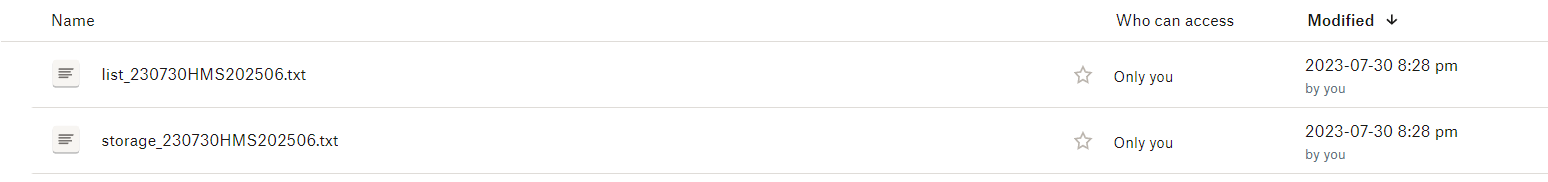
\includegraphics{content/material/ch2/check_dropbox_upload.png}

\subsection{Check the WiFi adapter going on monitor
mode}\label{check-the-wifi-adapter-going-on-monitor-mode}

In monitor mode, the WiFi adapter's status light should turn off, and
its connection will vanish from your mobile hotspot interface.

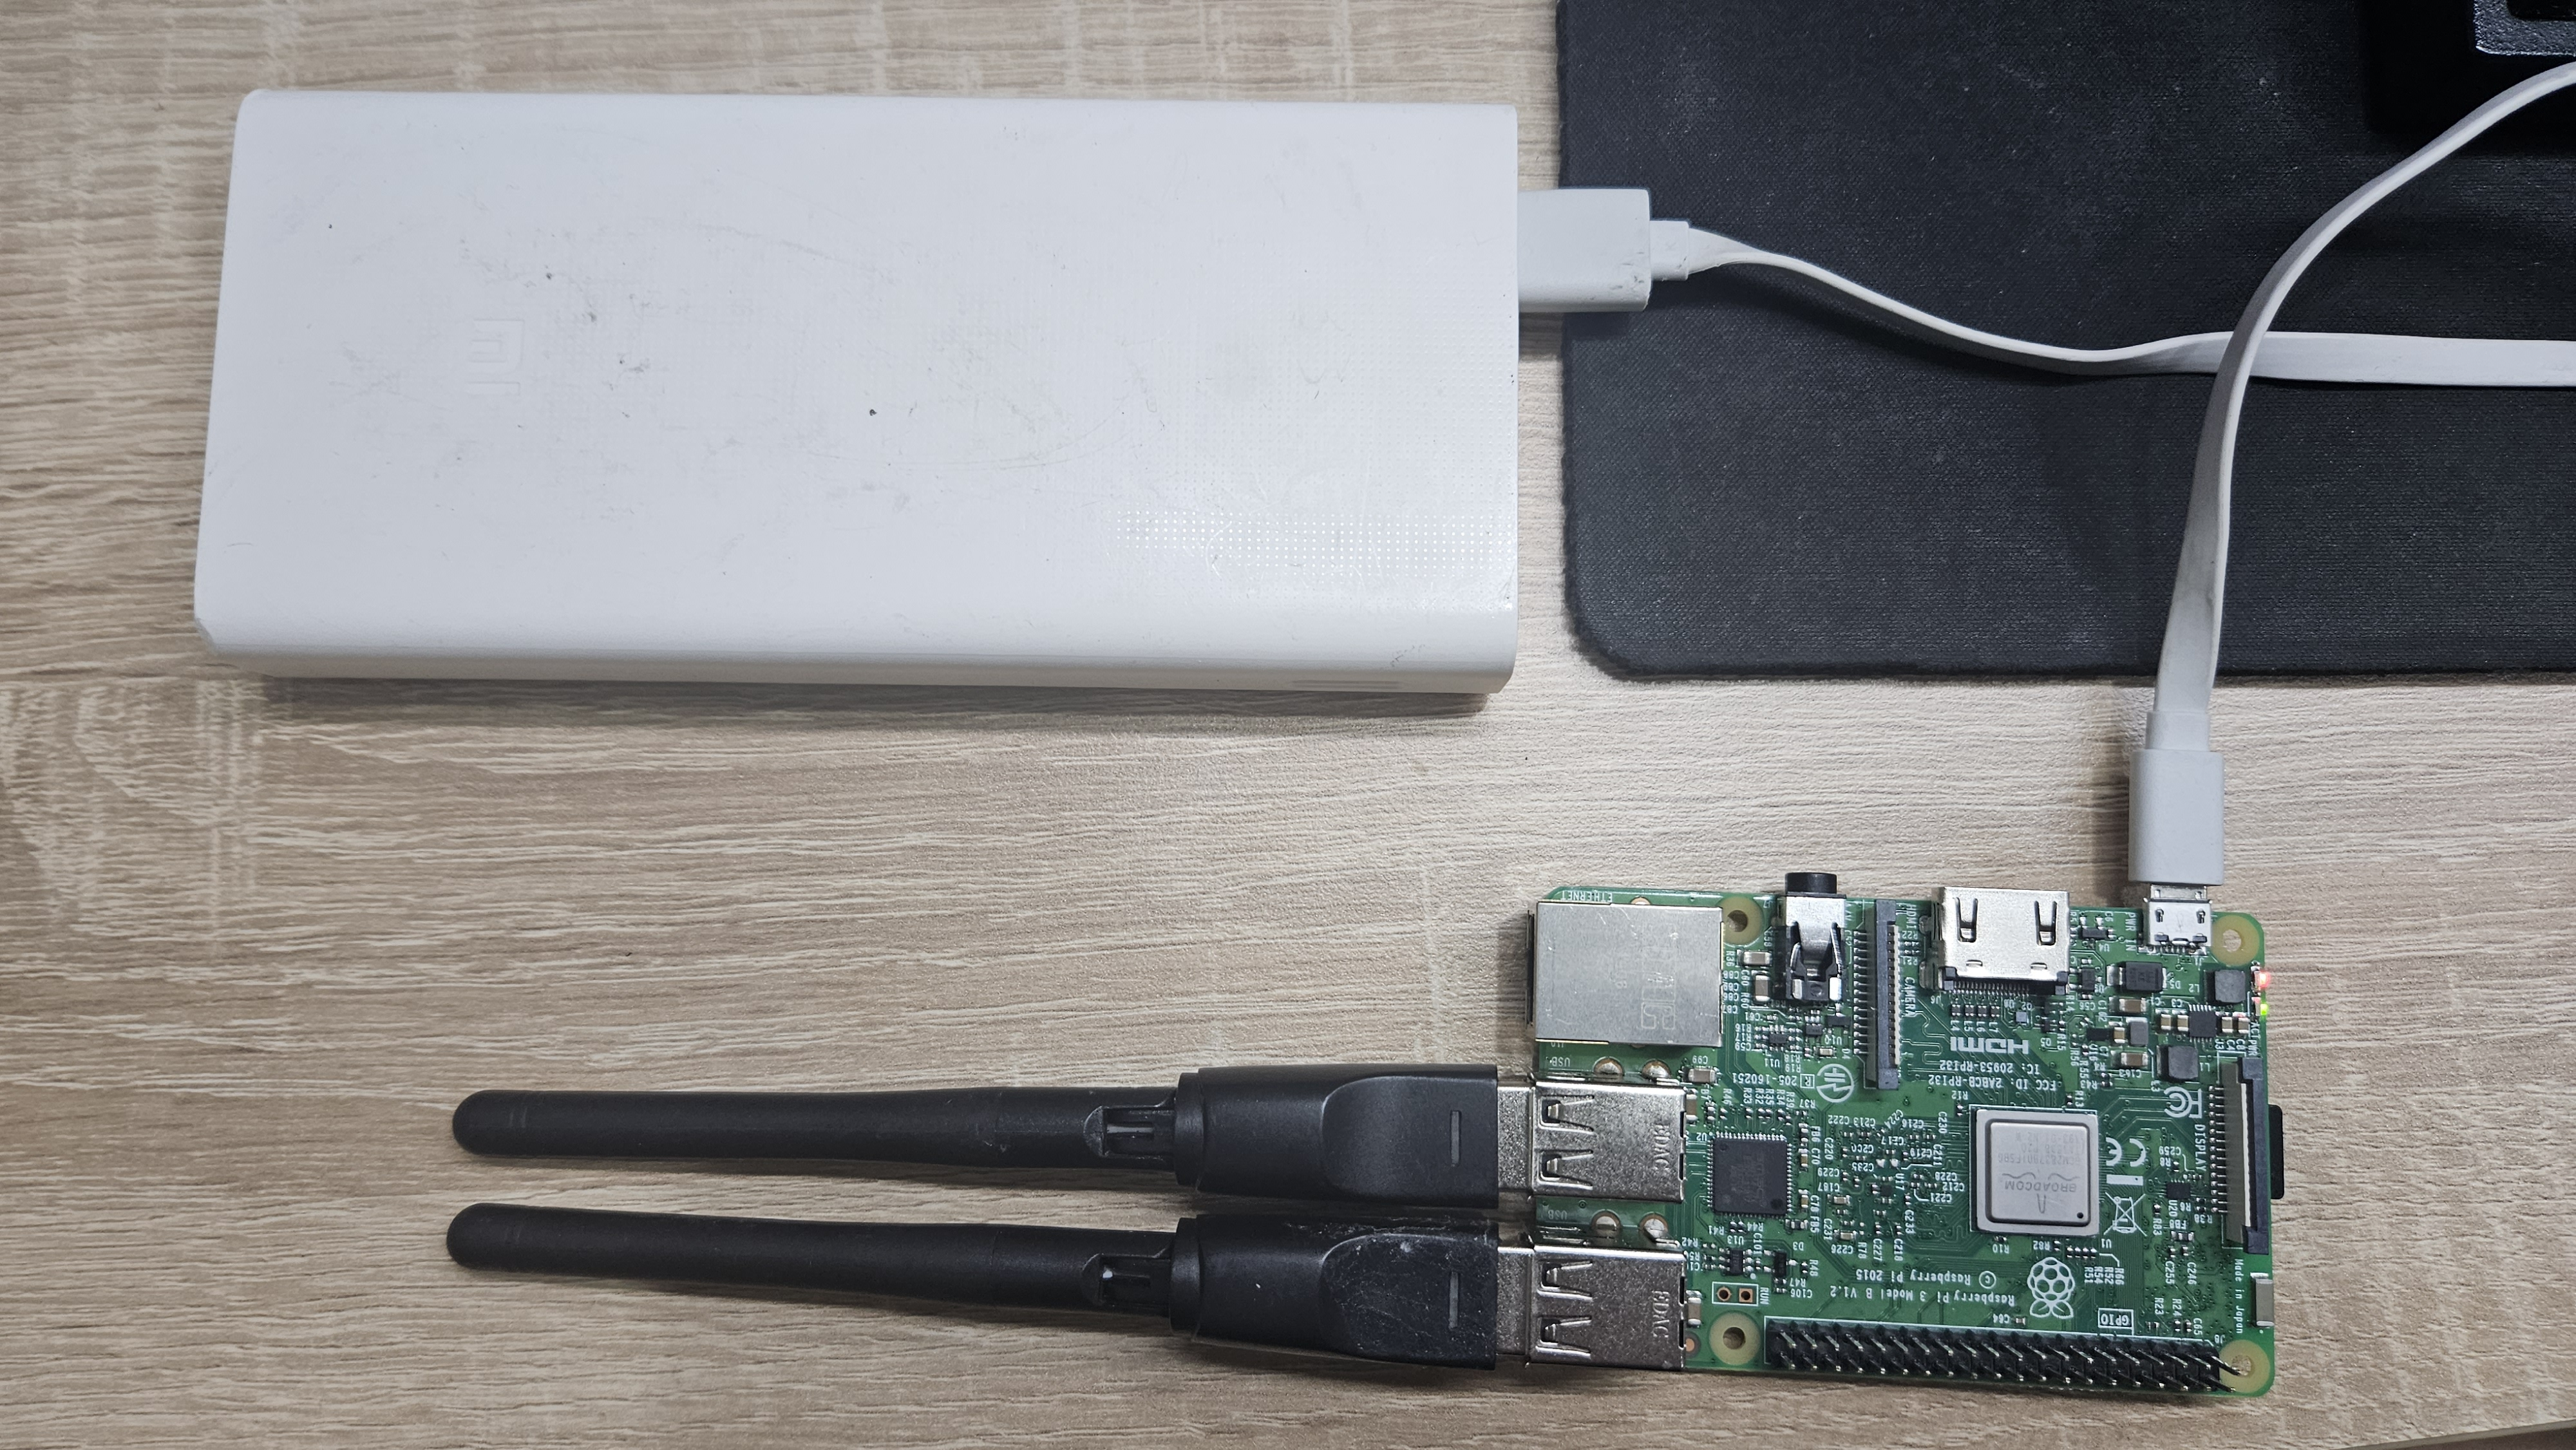
\includegraphics{content/material/ch2/plug_external.jpg}

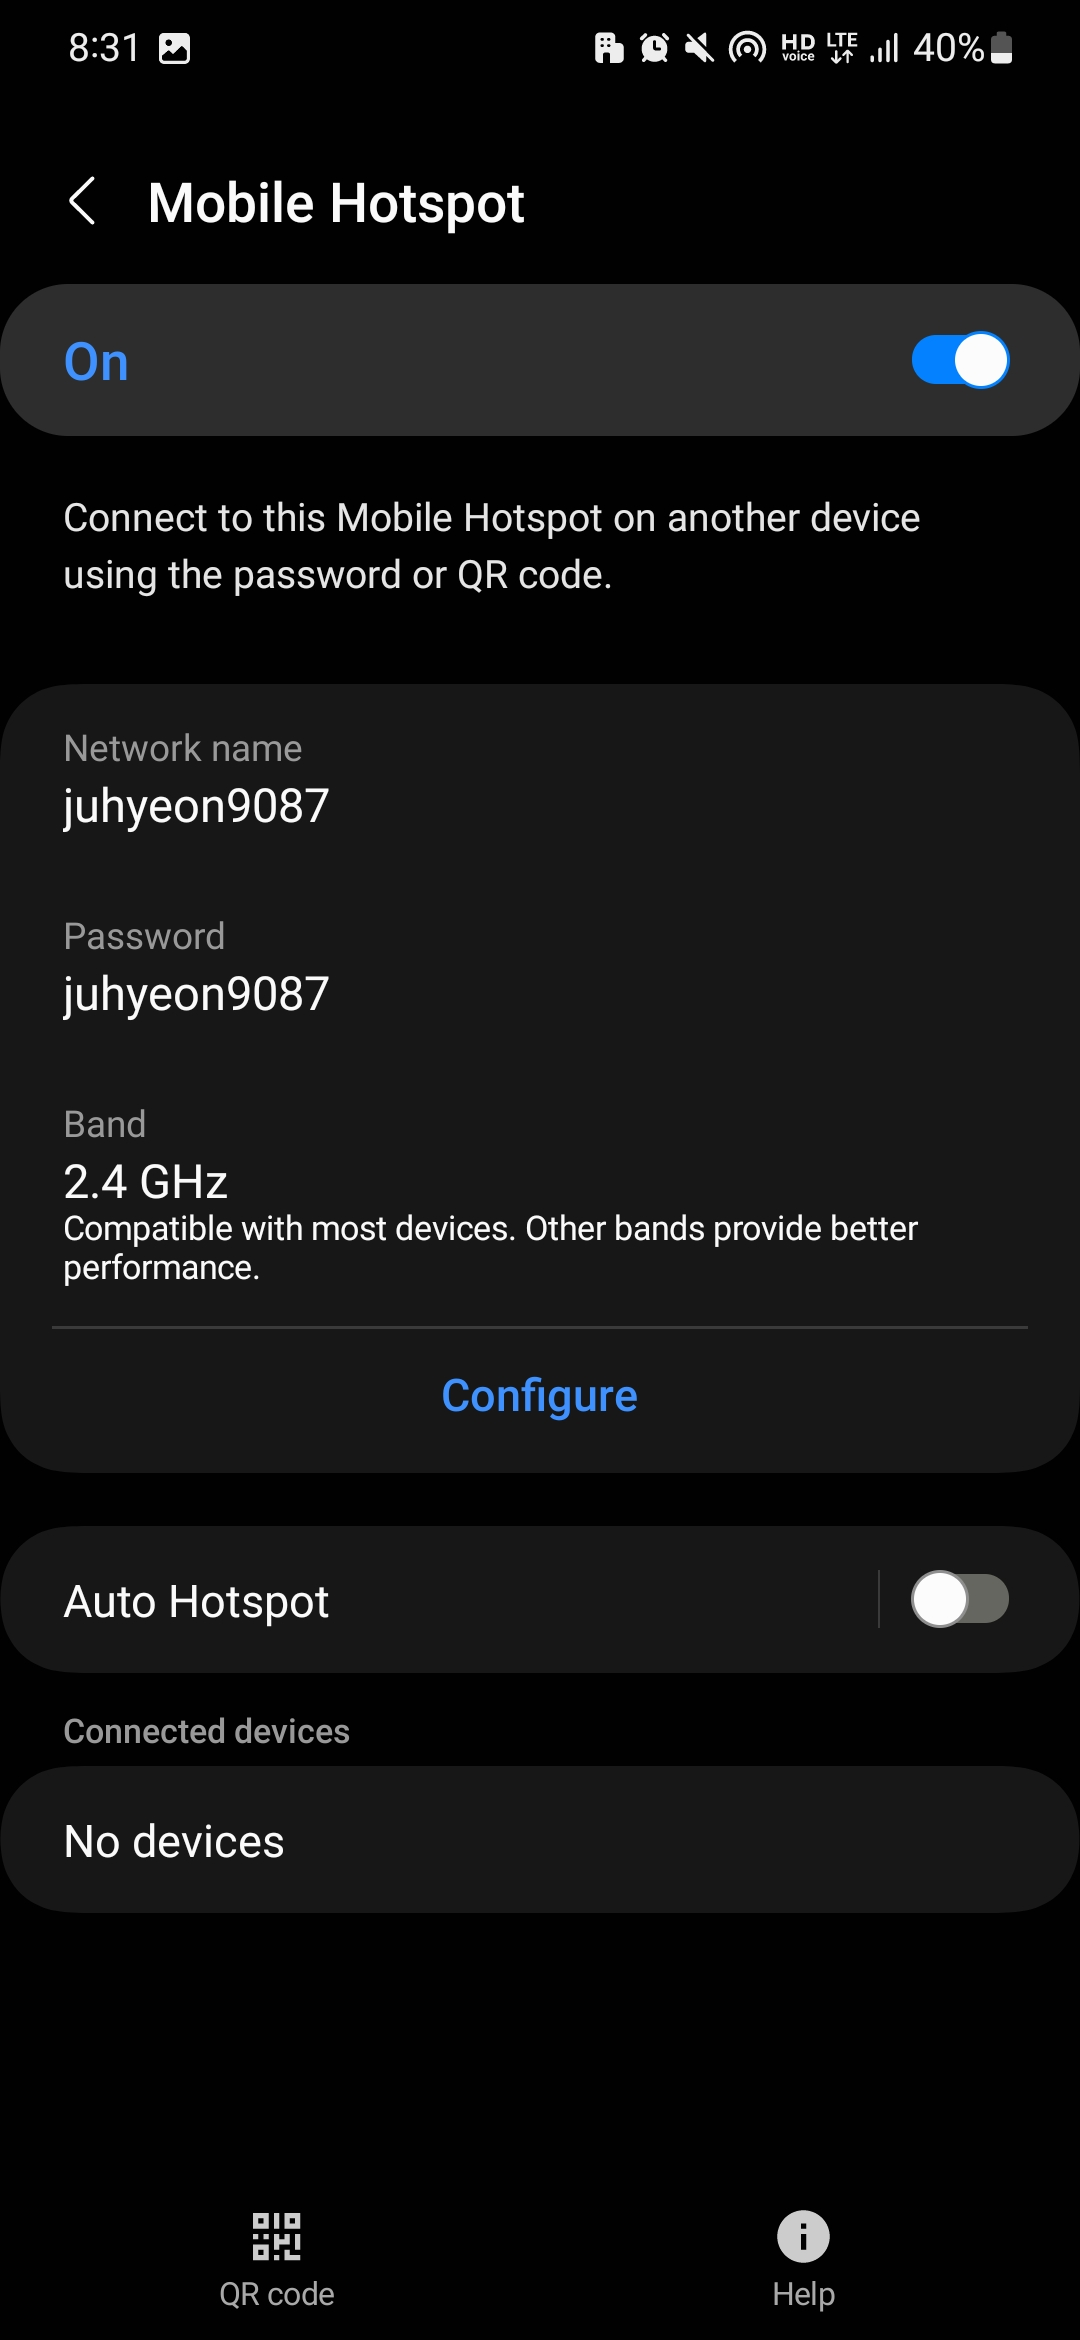
\includegraphics[width=0.5\textwidth,height=\textheight]{content/material/ch2/check_hotspot_off.jpg}

\subsection{Wait for Sensing
Operation}\label{wait-for-sensing-operation}

Throughout the designated sensing duration, the service will capture
packets.

\subsection{End Sensing Operation}\label{end-sensing-operation}

To conclude the sensing operation, simply unplug the battery.

\subsection{Review Sensing Results}\label{review-sensing-results}

Use Ethernet or your mobile phone hotspot to access and review the
generated sensing results, as same to the controlled enviroment testing.

\includegraphics{content/material/ch2/final_check.mp4}

\part{PART III: Data Collection and Processing}

\chapter{Data Collection Insights}\label{data-collection-insights}

\section{Understanding WiFi Sensing
Types}\label{understanding-wifi-sensing-types}

WiFi, a technology for wireless networking based on IEEE 802.11
standards, can be used to measure people's location and behavior through
two main approaches: passive and active WiFi sensing.

\includegraphics{content/material/ch3/wifi-sensing-types.png}

\textbf{Passive WiFi sensing} is a receive-only system that captures
WiFi packets emitted from WiFi-enabled devices carried by individuals.
It focuses on answering \emph{``Where is the station and its holder?''}
without requiring active participation from the person. Sensors
(sniffers) or access points (APs) detect WiFi packets sent from nearby
devices, which regularly emit WiFi packets to discover nearby APs, even
when not connected (Bonné et al., 2013; Musa \& Eriksson, 2012). The
typical detection range is approximately 100 meters, considering
commercial sensor specifications and WiFi device transmission range
(Chilipirea, 2019).

On the other hand, \textbf{active WiFi sensing} is a geolocation system
that uses WiFi packets from nearby APs to determine the location of a
device. It focuses on answering \emph{``Where am I?''} from the device's
perspective. The device scans for nearby WiFi APs and saves received
packets, which are then sent to a server for location estimation and
transmitted back to the device. Active sensing requires user consent and
active participation, such as installing an application to collect and
send WiFi logs.

\subsection*{Passive Sensing for Pedestrian Behavior
Monitoring}\label{passive-sensing-for-pedestrian-behavior-monitoring}
\addcontentsline{toc}{subsection}{Passive Sensing for Pedestrian
Behavior Monitoring}

This book focuses on passive WiFi sensing for studying pedestrian
behavior in urban environments. As illustrated in Figure 6-1, passive
sensing aims to answer the question \emph{``Where is the station and its
holder?''} without requiring active participation from individuals. This
approach is particularly suitable for urban planning and research, where
it is impractical to ask for consent from the numerous pedestrians using
public spaces.

Passive sensing offers a non-intrusive and scalable method for gathering
data on pedestrian behavior by capturing the WiFi packets emitted by
devices carried by pedestrians. This data provides valuable insights
into pedestrian movement patterns, space utilization, and social
interactions in urban environments, enabling better planning, design,
and management of public spaces. In contrast, active sensing focuses on
answering ``Where am I?'' from the device's perspective, which requires
user consent and active participation. While active sensing allows for
richer data on people's mobility, it is less practical for large-scale
pedestrian behavior monitoring in urban environments.

However, it is essential to consider the limitations, privacy concerns,
and ethical implications of passive WiFi sensing. While individuals are
not actively providing information, the collection of WiFi packets from
their devices may still raise privacy concerns. Researchers should
ensure that the data collection process is transparent, secure, and
complies with relevant privacy regulations.

\section{Sensor Installation
Strategies}\label{sensor-installation-strategies}

One of the most convenient and discreet ways to install WiFi sensors
outdoors is by attaching them to existing street furniture, such as
trees or lampposts. Make sure to use waterproof enclosures and secure
the sensors firmly to minimize the risk of damage from weather
conditions or tampering. This approach allows you to leverage existing
infrastructure in the urban environment while keeping the sensors out of
sight. Figure 6-2 shows an example of a sensor attached to a lamppost.

\section{Sensor Placement Strategies}\label{sensor-placement-strategies}

To optimize coverage and minimize signal interference, consider the
following strategies when deciding where to place your WiFi sensors:

\begin{itemize}
\tightlist
\item
  Single street coverage: If your target area is a single street, place
  sensors at both ends and a few in the middle to ensure adequate
  coverage along the entire length of the street.
\item
  District-wide coverage: When monitoring a larger area such as a
  district, position sensors at intersections to maximize coverage and
  capture pedestrian movement patterns between different streets and
  areas.
\item
  Avoiding interference: Steer clear of areas with high levels of
  electromagnetic interference, such as electrical equipment or large
  metal structures, to maintain signal quality and reliability.
\item
  Indoor considerations: When installing sensors indoors, account for
  signal attenuation caused by walls and other obstacles, as this can
  affect the range and accuracy of the sensors.
\item
  Outdoor protection: In outdoor environments, minimize the impact of
  weather conditions by shielding sensors from direct exposure to rain,
  snow, or extreme temperatures.
\item
  Accessibility and security: Place sensors in locations that are easily
  accessible for maintenance and troubleshooting, while also ensuring
  the security of the sensors to prevent tampering or damage.
\end{itemize}

\section{Optimizing Sensor Density for
Accuracy}\label{optimizing-sensor-density-for-accuracy}

The number and density of sensors play a crucial role in determining the
accuracy and reliability of the WiFi sensing system. While a higher
number of sensors generally leads to improved accuracy, it is essential
to strike a balance between performance and practical considerations,
such as cost and maintenance.

As a general guideline for outdoor deployments, aim to install sensors
at intervals of approximately 100 meters. This means placing one sensor
for every 100 meters of the target area. While more sensors can enhance
accuracy, this spacing has been found to provide a good balance between
performance and resource efficiency based on experimental results.

Detailed Experiment on Sensor Density (click to expand)

A study conducted in the central street of the University of Ulsan
retail district tested the effects of sensor density on localization
performance and the number of detected samples. The study created
scenarios with varying sensor densities (Table 6-1) and found that lower
sensor density led to poorer localization performance (Figure 6-3) and a
decreased percentage of detected samples (Figure 6-4).

Table 6-1. Description of scenarios based on sensor locations and counts

Scenario Number of locations Number of sensors Average distance
Description Baseline 7 8 53.6m Default experiment setting Scenario 1 4 5
107m Removes 3 locations Scenario 2 3 3 161m Removes 1 location Scenario
3 2 2 322m Removes 1 location Figure 6-3. Localization performance by
scenario (30 seconds sampling time) Figure 6-4. Localization error and
number of samples used by scenario when localized to 30 seconds of
sampling

By following these sensor installation tips and strategies, even those
new to WiFi sensing can effectively deploy sensors for pedestrian
behavior monitoring, ensuring high-quality data collection and accurate
localization performance. Remember, the key is to find the right balance
between sensor density, placement, and practical considerations to
create a reliable and efficient WiFi sensing system.

\chapter{Data Structure and Loading}\label{data-structure-and-loading}

In this section, we will first examine the raw WiFi data stored in an
SQLite3 database and then demonstrate how to load this data into R for
further processing.

\section{Data Structure}\label{data-structure}

\section{Overview of Filtering
Techniques}\label{overview-of-filtering-techniques}

The three filtering techniques used for WiFi data preprocessing are:

\textbf{1. Removal of random MAC addresses:} Eliminates random MAC
addresses to avoid duplicate counting.

\textbf{2. Removal of non-mobile devices:} Removes detection records of
static devices to focus on mobility.

\textbf{3. Removal of rarely detected devices:} Excludes MAC addresses
that are detected for very short duration.

\includegraphics{content/material/ch3/preprocessing.png}

\section{Raw Data Structure}\label{raw-data-structure}

The raw data is typically stored in a structured format, such as a
database or a comma-separated values (CSV) file. For this example, let's
assume the data is stored in an SQLite3 database. The database may
contain one or more tables that capture the WiFi sensing data.

Each row in the dataset represents a captured WiFi packet, and the
columns provide various attributes of the packet:

\begin{itemize}
\tightlist
\item
  Timestamp: The timestamp indicates when the packet was captured,
  allowing for temporal analysis.
\item
  Type and Subtype: These columns specify the type and subtype of the
  captured packet. In this example, the packets are management frames
  with a subtype of probe-request, indicating that devices are searching
  for nearby APs.
\item
  Strength: The signal strength of the received packet is recorded in
  dBm units, providing information about the proximity of the device to
  the sensor.
\item
  Source Address: The source address is the hashed MAC address of the
  device sending the packet, enabling device identification while
  preserving privacy.
\item
  Source Randomized: This column indicates whether the source address is
  randomized (1) or not (0).
\item
  Destination Address: The destination address is the hashed MAC address
  of the intended recipient of the packet.
\item
  Destination Randomized: This column indicates whether the destination
  address is randomized (1) or not (0).
\item
  Access Point Name: The name of the access point (AP) that the device
  is trying to discover.
\item
  Access Point Address: The hashed MAC address of the AP.
\item
  Access Point Randomized: This column indicates whether the AP address
  is randomized (1) or not (0).
\item
  Sequence Number: The sequence number of the packet, used for ordering
  and identifying packets within a sequence.
\item
  Channel: The WiFi channel on which the packet was transmitted.
\item
  Sensor Name: The name of the sensor that captured the packet.
\end{itemize}

\chapter{Preprocessing Techniques}\label{preprocessing-techniques}

With a clear understanding of the raw WiFi data structure, we can now
proceed with data preprocessing techniques to clean, transform, and
prepare the data for analysis. In this section, we will first
demonstrate how to load the WiFi data into R and then discuss various
preprocessing techniques to improve data quality and analysis results.

\section{Loading WiFi Data with R}\label{loading-wifi-data-with-r}

We need to load the raw WiFi data from the SQLite3 database into R using
the RSQLite and DBI packages.

For a more streamlined and efficient process, we'll utilize the pacman
package, which offers the \texttt{p\_load} function. This function
automatically installs and loads the necessary packages if they are not
already installed.

First, ensure the \texttt{pacman} package is installed and loaded:

\begin{Shaded}
\begin{Highlighting}[]
\ControlFlowTok{if}\NormalTok{ (}\SpecialCharTok{!}\FunctionTok{require}\NormalTok{(pacman)) }\FunctionTok{install.packages}\NormalTok{(}\StringTok{"pacman"}\NormalTok{)}
\end{Highlighting}
\end{Shaded}

\begin{verbatim}
필요한 패키지를 로딩중입니다: pacman
\end{verbatim}

\begin{Shaded}
\begin{Highlighting}[]
\NormalTok{pacman}\SpecialCharTok{::}\FunctionTok{p\_load}\NormalTok{(pacman)}
\end{Highlighting}
\end{Shaded}

Next, use \texttt{p\_load} from \texttt{pacman} to install and load the
\texttt{RSQLite} and \texttt{DBI} packages, essential for interfacing
with SQLite databases:

\begin{Shaded}
\begin{Highlighting}[]
\NormalTok{pacman}\SpecialCharTok{::}\FunctionTok{p\_load}\NormalTok{(RSQLite, DBI, data.table, knitr)}
\end{Highlighting}
\end{Shaded}

Next, establish a connection to your SQLite3 database using the
dbConnect() function:

\begin{Shaded}
\begin{Highlighting}[]
\NormalTok{conn }\OtherTok{\textless{}{-}} \FunctionTok{dbConnect}\NormalTok{(}\FunctionTok{SQLite}\NormalTok{(), }\StringTok{"path/to/your/database.sqlite"}\NormalTok{)}
\end{Highlighting}
\end{Shaded}

Replace \texttt{"path/to/your/database.sqlite"} with the actual path to
your SQLite3 database file.

\begin{tcolorbox}[enhanced jigsaw, opacityback=0, colbacktitle=quarto-callout-note-color!10!white, toptitle=1mm, colframe=quarto-callout-note-color-frame, rightrule=.15mm, title=\textcolor{quarto-callout-note-color}{\faInfo}\hspace{0.5em}{If you don't have the WiFi DB}, toprule=.15mm, colback=white, bottomrule=.15mm, coltitle=black, breakable, leftrule=.75mm, left=2mm, opacitybacktitle=0.6, bottomtitle=1mm, arc=.35mm, titlerule=0mm]

Download \href{material/ch3/sample.sqlite3}{this}

\end{tcolorbox}

To load the WiFi data from the ``packets'' table, use the dbGetQuery()
function:

\begin{Shaded}
\begin{Highlighting}[]
\NormalTok{wifi\_data }\OtherTok{\textless{}{-}} \FunctionTok{dbGetQuery}\NormalTok{(conn, }\StringTok{"SELECT * FROM packets"}\NormalTok{)}
\end{Highlighting}
\end{Shaded}

\begin{longtable}[]{@{}
  >{\raggedright\arraybackslash}p{(\columnwidth - 28\tabcolsep) * \real{0.0662}}
  >{\raggedright\arraybackslash}p{(\columnwidth - 28\tabcolsep) * \real{0.0270}}
  >{\raggedright\arraybackslash}p{(\columnwidth - 28\tabcolsep) * \real{0.0368}}
  >{\raggedleft\arraybackslash}p{(\columnwidth - 28\tabcolsep) * \real{0.0221}}
  >{\raggedright\arraybackslash}p{(\columnwidth - 28\tabcolsep) * \real{0.1593}}
  >{\raggedleft\arraybackslash}p{(\columnwidth - 28\tabcolsep) * \real{0.0637}}
  >{\raggedright\arraybackslash}p{(\columnwidth - 28\tabcolsep) * \real{0.1593}}
  >{\raggedleft\arraybackslash}p{(\columnwidth - 28\tabcolsep) * \real{0.0760}}
  >{\raggedright\arraybackslash}p{(\columnwidth - 28\tabcolsep) * \real{0.0515}}
  >{\raggedright\arraybackslash}p{(\columnwidth - 28\tabcolsep) * \real{0.1593}}
  >{\raggedleft\arraybackslash}p{(\columnwidth - 28\tabcolsep) * \real{0.0784}}
  >{\raggedleft\arraybackslash}p{(\columnwidth - 28\tabcolsep) * \real{0.0392}}
  >{\raggedright\arraybackslash}p{(\columnwidth - 28\tabcolsep) * \real{0.0196}}
  >{\raggedright\arraybackslash}p{(\columnwidth - 28\tabcolsep) * \real{0.0294}}
  >{\raggedright\arraybackslash}p{(\columnwidth - 28\tabcolsep) * \real{0.0123}}@{}}
\toprule\noalign{}
\begin{minipage}[b]{\linewidth}\raggedright
timestamp
\end{minipage} & \begin{minipage}[b]{\linewidth}\raggedright
type
\end{minipage} & \begin{minipage}[b]{\linewidth}\raggedright
subtype
\end{minipage} & \begin{minipage}[b]{\linewidth}\raggedleft
strength
\end{minipage} & \begin{minipage}[b]{\linewidth}\raggedright
source\_address
\end{minipage} & \begin{minipage}[b]{\linewidth}\raggedleft
source\_address\_randomized
\end{minipage} & \begin{minipage}[b]{\linewidth}\raggedright
destination\_address
\end{minipage} & \begin{minipage}[b]{\linewidth}\raggedleft
destination\_address\_randomized
\end{minipage} & \begin{minipage}[b]{\linewidth}\raggedright
access\_point\_name
\end{minipage} & \begin{minipage}[b]{\linewidth}\raggedright
access\_point\_address
\end{minipage} & \begin{minipage}[b]{\linewidth}\raggedleft
access\_point\_address\_randomized
\end{minipage} & \begin{minipage}[b]{\linewidth}\raggedleft
sequence\_number
\end{minipage} & \begin{minipage}[b]{\linewidth}\raggedright
channel
\end{minipage} & \begin{minipage}[b]{\linewidth}\raggedright
sensor\_name
\end{minipage} & \begin{minipage}[b]{\linewidth}\raggedright
info
\end{minipage} \\
\midrule\noalign{}
\endhead
\bottomrule\noalign{}
\endlastfoot
2024-04-09T19:17:27.536121 & management & probe-response & -65 &
f0659bdd9305e4341afb9f55df7cd20a4adfd726f83a33c3857281dfa3de8575 & 0 &
767dcce0bef280209ebb9401ddd0694ebd4ca7c7703e3c0269cb86d6592e0012 & 1 &
SK\_WiFiGIGA8161\_2.4G &
f0659bdd9305e4341afb9f55df7cd20a4adfd726f83a33c3857281dfa3de8575 & 0 &
604 & 6 & A01 & \\
2024-04-09T19:17:27.541249 & management & probe-response & -67 &
f0659bdd9305e4341afb9f55df7cd20a4adfd726f83a33c3857281dfa3de8575 & 0 &
767dcce0bef280209ebb9401ddd0694ebd4ca7c7703e3c0269cb86d6592e0012 & 1 &
SK\_WiFiGIGA8161\_2.4G &
f0659bdd9305e4341afb9f55df7cd20a4adfd726f83a33c3857281dfa3de8575 & 0 &
607 & 6 & A01 & \\
2024-04-09T19:17:27.635933 & management & probe-response & -67 &
f0659bdd9305e4341afb9f55df7cd20a4adfd726f83a33c3857281dfa3de8575 & 0 &
00333fd8244862428d22a482df516ae0315c33a83a9d32e9bf8bc2b0de978467 & 1 &
SK\_WiFiGIGA8161\_2.4G &
f0659bdd9305e4341afb9f55df7cd20a4adfd726f83a33c3857281dfa3de8575 & 0 &
611 & 6 & A01 & \\
2024-04-09T19:17:27.746452 & management & probe-request & -67 &
d94147cf12befe41bb40dd7957733c54442de7a9d45a75ec3c747856c4bdc129 & 1 &
ff:ff:ff:ff:ff:ff & 1 & (n/a) & ff:ff:ff:ff:ff:ff & 1 & 990 & 1 & A01
& \\
2024-04-09T19:17:27.765945 & management & probe-request & -65 &
d94147cf12befe41bb40dd7957733c54442de7a9d45a75ec3c747856c4bdc129 & 1 &
ff:ff:ff:ff:ff:ff & 1 & (n/a) & ff:ff:ff:ff:ff:ff & 1 & 991 & 1 & A01
& \\
\end{longtable}

After loading the data, remember to close the database connection:

\begin{Shaded}
\begin{Highlighting}[]
\FunctionTok{dbDisconnect}\NormalTok{(conn)}
\end{Highlighting}
\end{Shaded}

\section{Filltering Techniques}\label{filltering-techniques}

The three filtering techniques used for WiFi data preprocessing are:

\textbf{1. Removal of random MAC addresses:} Eliminates random MAC
addresses to avoid duplicate counting.

\textbf{2. Removal of non-mobile devices:} Removes detection records of
static devices to focus on mobility.

\textbf{3. Removal of rarely detected devices:} Excludes MAC addresses
that are detected for very short duration.

\includegraphics{content/material/ch3/preprocessing.png}

\subsection{(Step 1) Removal of Random MAC
Addresses}\label{step-1-removal-of-random-mac-addresses}

Random MAC addresses are identified by matching the OUI
(Organizationally Unique Identifier) portion of the MAC address with a
public database provided by IEEE. The OUI is the first 6 digits of a MAC
address, representing the device manufacturer. Unmatched OUIs are
considered random MAC addresses and are removed.

\subsection{(Step 2) Removal of Non-Mobile
Devices}\label{step-2-removal-of-non-mobile-devices}

\subsection{(Step 3) Removal of Rarely Detected
Devices}\label{step-3-removal-of-rarely-detected-devices}

\part{PART III: Understanding Metrics}

\chapter{Metrics Overview}\label{metrics-overview}

We explore how WiFi gives us a snapshot of life in the city. It's about
finding where people are (\emph{\textbf{Location}}), tallying up the
numbers (\emph{\textbf{Count}}), tracking movement
(\emph{\textbf{Track}}), identifying patterns
(\emph{\textbf{Identify}}), and figuring out actions
(\emph{\textbf{Activities}}). A graphic will illustrate these concepts
step by step:

\begin{figure}[H]

{\centering \includegraphics{content/material/ch4/metric-overview.png}

}

\caption{Overview of WiFi Sensing Metrics: From Pinpointing Locations to
Understanding Urban Activities}

\end{figure}%

\subsubsection*{\texorpdfstring{\textbf{Ground Truth: What's really
happening?}}{Ground Truth: What's really happening?}}\label{ground-truth-whats-really-happening}
\addcontentsline{toc}{subsubsection}{\textbf{Ground Truth: What's really
happening?}}

We start with the `Ground Truth'---observing what's actually happening
on the ground. This real-life observation helps us check and confirm our
WiFi data findings. It's the benchmark against which we measure the
accuracy of our WiFi sensing data.

\subsubsection*{\texorpdfstring{\textbf{Location: Where are people at a
specific
time?}}{Location: Where are people at a specific time?}}\label{location-where-are-people-at-a-specific-time}
\addcontentsline{toc}{subsubsection}{\textbf{Location: Where are people
at a specific time?}}

`Location' is determined by analyzing the characteristics of WiFi
signals at a given time, like signal frequency and strength. Depending
on the situation, we might assign locations based on sensor positions or
estimate them in areas between sensors.

\begin{tcolorbox}[enhanced jigsaw, opacityback=0, colbacktitle=quarto-callout-note-color!10!white, toptitle=1mm, colframe=quarto-callout-note-color-frame, rightrule=.15mm, title=\textcolor{quarto-callout-note-color}{\faInfo}\hspace{0.5em}{Why Location Comes Before Count}, toprule=.15mm, colback=white, bottomrule=.15mm, coltitle=black, breakable, leftrule=.75mm, left=2mm, opacitybacktitle=0.6, bottomtitle=1mm, arc=.35mm, titlerule=0mm]

Before counting, we must pinpoint location. Without knowing where
devices are, we just have a total count.

Imagine a room with three people, just like in the diagram above:

\begin{itemize}
\tightlist
\item
  \textbf{Without location data,} counting detected device MAC addresses
  only tells you there are three devices total.
\item
  \textbf{With even rough location data,} you can determine that two
  devices are on the left and one on the right -- providing much richer
  information.
\end{itemize}

\end{tcolorbox}

\subsubsection*{\texorpdfstring{\textbf{Count: How many over
time?}}{Count: How many over time?}}\label{count-how-many-over-time}
\addcontentsline{toc}{subsubsection}{\textbf{Count: How many over
time?}}

`Count' focuses on tallying unique MAC addresses to estimate how many
people are in an area over different timescales. This method allows for
long-term tracking of device presence, offering insights into occupancy
trends over extended periods.

\subsubsection*{\texorpdfstring{\textbf{Track: Where and when did they
move?}}{Track: Where and when did they move?}}\label{track-where-and-when-did-they-move}
\addcontentsline{toc}{subsubsection}{\textbf{Track: Where and when did
they move?}}

`Track' involves recording when and where phones are detected. This data
lets us follow people's movements, highlighting the dynamic patterns of
city life and offering insights into how different areas are used
throughout the day.

\subsubsection*{\texorpdfstring{\textbf{Identify: Who visits regularly
and what are their
patterns?}}{Identify: Who visits regularly and what are their patterns?}}\label{identify-who-visits-regularly-and-what-are-their-patterns}
\addcontentsline{toc}{subsubsection}{\textbf{Identify: Who visits
regularly and what are their patterns?}}

With `Identify', we analyze data over time to recognize regular visitors
and understand their movement habits. This metric provides insights into
recurring traffic patterns and the behaviors of different user groups
within the city.

\subsubsection*{\texorpdfstring{\textbf{Activities: What are they doing
and how does it
change?}}{Activities: What are they doing and how does it change?}}\label{activities-what-are-they-doing-and-how-does-it-change}
\addcontentsline{toc}{subsubsection}{\textbf{Activities: What are they
doing and how does it change?}}

`Activities' aims to understand actions by analyzing timing and movement
data. We look at how people use different city areas, observing changes
in activity patterns at different times and days, to get a deeper
understanding of urban life.

\chapter{Count}\label{count}

\chapter{Track}\label{track}

\chapter{Identity}\label{identity}

\chapter{Activities}\label{activities}

\part{PART VI: Applying Metrics}

\chapter{Case Study 1}\label{case-study-1}

\chapter{Case Study 2}\label{case-study-2}

\chapter{Case Study 3}\label{case-study-3}

\part{PART V: Future Directions and Challenges}

\chapter{Limitation}\label{limitation}

\chapter{Direction}\label{direction}

\part{Further}


\backmatter

\end{document}
